% Created 2016-02-08 月 21:44
\documentclass[a4j,12pt,oneside,openany,english]{jsbook}
\usepackage{graphicx}
\usepackage{amssymb}
\usepackage{amsmath}
\usepackage{latexsym}
\usepackage{book2report}
\usepackage{thesis}

\usepackage{amssymb}
\usepackage{multirow}
\usepackage{threeparttable}
\usepackage{array}
\usepackage{color}

\usepackage{lscape}

\usepackage{nidanfloat}
\usepackage{setspace}

\usepackage{float}
\usepackage{here}

\usepackage{listings}
\lstset{
	%プログラム言語(複数の言語に対応,Python,C,C++も可)
 	language = C++,
 	%背景色と透過度
 	backgroundcolor={\color[gray]{.70}},
 	%枠外に行った時の自動改行
 	breaklines = true,
 	%自動改行後のインデント量(デフォルトでは20[pt])	
 	breakindent = 10pt,
 	%標準の書体
 	basicstyle = \ttfamily\scriptsize,
 	%コメントの書体
 	commentstyle = {\itshape \color[cmyk]{1,0.4,1,0}},
 	%関数名等の色の設定
 	classoffset = 0,
 	%キーワード(int, ifなど)の書体
 	keywordstyle = {\bfseries \color[cmyk]{0,1,0,0}},
 	%表示する文字の書体
 	stringstyle = {\ttfamily \color[rgb]{0,0,1}},
 	%枠 "t"は上に線を記載, "T"は上に二重線を記載
	%他オプション:leftline,topline,bottomline,lines,single,shadowbox
 	frame = TBrl,
 	%frameまでの間隔(行番号とプログラムの間)
 	framesep = 5pt,
 	%行番号の位置
 	numbers = left,
	%行番号の間隔
 	stepnumber = 1,
	%行番号の書体
 	numberstyle = \tiny,
	%タブの大きさ
 	tabsize = 4,
 	%キャプションの場所("tb"ならば上下両方に記載)
 	captionpos = b
}

% \newcommand{\comment}[1]{\colorbox{green}{#1}}
\newcommand{\comment}[1]{}
% \newcommand{\memo}[1]{\colorbox{green}{#1} \\ }
\newcommand{\memo}[1]{}


\setcounter{topnumber}{5}%    ページ上部の図表は 5 個まで
\def\topfraction{1.00}%       ページの上 1.00 まで図表で占めて可
\setcounter{bottomnumber}{5}% ページ下部の図表は 5 個まで
\def\bottomfraction{1.00}%    ページの下 1.00 まで図表で占めて可
\setcounter{totalnumber}{10}% ページあたりの図表は 10 個まで
\def\textfraction{0.00}%      ページうち本文が占める割合の下限
  

\date{\today}
\begin{document}

% 英語で,見出しのフォントが気に入らなかったら
\renewcommand{\headfont}{\bfseries}

% ページ数が少ないときはここを大きくしてごまかそう!!効果絶大!!
% \renewcommand{\baselinestretch}{1.1}

%%%%%%%%%%%% 題目 %%%%%%%%%%%%%%%%%%%%%%%%%%%%%%%%%%%%%%%%%%%%%%%%%%%%%%%
%%%%%%%%%%%% ここも適当に変えてもいいと思う %%%%%%%%%%%%%%%%%%%%%%%%%%%%%%%%%
\thispagestyle{empty}
\begin{center}
  \vspace*{5mm}
  {\Huge {\bf Master's Thesis}}\\
  \vspace{2cm}
  \vspace{1cm}
  \underline{\LARGE{Scalable Parallel Computing}} \\
  \vspace{0.2cm}
  \underline{\LARGE{on NoC-based Embedded Many-Core Platform}} \\  
  \vspace{0.5cm}
  \vspace{12mm}
  {\large Supervisor}\\
  \vspace{6mm}
  \underline{\Large Professor Toshimitsu Ushio}\\
   \\
  \underline{\Large Assistant Professor Takuya Azumi}\\
  \vspace{8mm}
  {\large By}\\
  \vspace{6mm}
  \underline{\Large Yuya Maruyama}\\
  \vspace{10mm}
  {\Large February 02, 2018}\\  
  \vspace{14mm}
  {\Large Division of Mathematical Science for Social System,}\\
  {\Large Department of Systems Innovation,}\\
  {\Large Graduate School of Engineering Science, Osaka University}\\
\end{center}
\clearpage
\setcounter{page}{0}
\pagenumbering{roman}

%%%%%%%%%%%% 概要 %%%%%%%%%%%%%%%%%%%%%%%%%%%%%%%%%%%%%%%%%%%%%%%%%%%%
\begin{abstract}
  This thesis summarizes the development and testing of ROS-lite, a parallel computing and software development framework for embedded computing platforms based on network-on-chip (NoC) technology.
  Such heterogeneous computing platforms are used because embedded systems often require powerful high processing capacity and low power consumption.
  Since they implement nonuniform memory access (NUMA) for scalability, software for many-core platforms must be designed based on scalable data allocation and scalable parallelization.
  % As a reference embedded many-core computing platform, we use the Massively Parallel Processor Arrays 256 (MPPA-256) developed by Kalray, one of the commercial off-the-shelf (COTS) multi-/many-core platforms.
  This thesis reports the results of data transfer tests on NoC implementations, microbenchmarks, and parallelization of self-driving software for implementation on an embedded many-core processor.
  ROS-lite, the proposed framework provides a structured communications layer for NoC components that reduces memory consumption and allows efficient software development for embedded many-core platforms.
  Using NUMA and the parallelization scalability of many cores, the data transfer latencies that are currently achievable between distributed memory resources are investigated.
  To test the practicality of embedded many-core platforms in a practical application, a module of a self-driving software suite is parallelized so that it can run on many-core processors.
  This pilot test achieves performance levels that are acceptable for market-ready autonomous vehicles.
  By highlighting many-core computing capabilities and efficient software development, I explore scalable parallel computing on NoC-based embedded many-core platforms.
\end{abstract}

%%%%%%%%%%%% 目次 %%%%%%%%%%%%%%%%%%%%%%%%%%%%%%%%%%%%%%%%%%%%%%%%%%%%
\clearpage
\tableofcontents
\clearpage
\setcounter{page}{0}
\pagenumbering{arabic}

%%%%%%%%%%%%% ここから内容 %%%%%%%%%%%%%%%%%%%%%%%%%%%%%%%%%%%%%%%%%%%%%%%%%%%%%%%%%%%%%%%%%%%%%%%%%%%%%%%%%%%%%%%%%%%%%%%%%%%%%%%%%%


% \setlength\textfloatsep{18pt}%  between figure and text
% \setlength\abovecaptionskip{4pt}% between figure and caption
% \setlength\floatsep{18pt}% between figures

\comment{TBD:1-1, 1-14, 2-2, 3-5}

% \IEEEraisesectionheading{\chapter{Introduction}\label{sec:introduction}}
\chapter{Introduction}
\label{sec:introduction}
\comment{1-4, 1-5, 1-6, 2-1, 2-4}
The evolution of a next-generation computing platform oriented toward having multi-/many-cores is necessary to satisfy the demand for increasing computation in conjunction with reasonable power consumption in several domains such as automobiles.
%%%%%%%%%%%%%%%%%%%%%%%%%%%%%%%%%%%%%%%%%%%%%%%  テンプレート非依存部(開始)  %%%%%%%%%%%%%%%%%%%%%%%%%%%%%%%%%%%%%%%%%%%%%%%  
This trend is also adapted to embedded systems because of high processing requirements.
For example, self-driving systems involve various applications and are sometimes characterized by demands for high-performance computing.
Considering the requirements of high processing, predictability, and energy efficiency for self-driving systems, such systems require a heterogeneous computing system such as multi-/many-core platforms and graphical processing units (GPU).
(This is discussed in Section \ref{sec:related_work}.)
\comment{1-3} In embedded systems, multi-/many-core architectures are an important trend as the architecture integrates cores to realize high-performance and general-purpose computing with low power consumption \cite{becker2016contention}, \cite{perret2016mapping}.
Extant studies have examined several applications of multi/many-core platforms \cite{becker2016contention}, \cite{saidi2015shift}, \cite{perret2016temporal}, \cite{perret2016mapping}, \cite{becker2014mapping} \cite{BURGIO2017299}.
% Recently, the computational ability of single core processors has reached its limit \comment{1-3} and thus the applicability of Moore's law \cite{moore2006cramming} is unclear.
% Multi/many core architecture is an important trend in \comment{1-3} recent years as it integrates cores to realize high-performance and general-purpose computing with low power consumption.
% Hence, high energy efficiency is a superior feature of multi/many core platforms.

% As detailed in the preceding paragraph, the demand for increasing computation in conjunction with reasonable power consumption drives the need for multi/many core architecture in several domains.
% Real-time embedded systems are an example in which multi/many core platforms are adopted since they face increasing processing requirements.
% Extant studies have examined numerous applications of multi/many cores platforms \cite{becker2016contention}, \cite{saidi2015shift}, \cite{perret2016temporal}, \cite{perret2016mapping}, \cite{becker2014mapping}.

% For example, automotive systems involve various applications and are sometimes characterized by demands for high-performance computing.
% Automotive applications are responsible for several control systems such as the powertrain, chassis, steering wheel, driver assistance and user interface.
% Advanced driver assistance systems are characterized by increasing complexity and computational requirements and necessitate intelligence such as an self-driving driving system.
% Moreover, they also require significant energy efficiency and cost reduction.
% Although modern automotive systems are composed of several Electronic Control Unit (ECU) managing subsystems, there is a shift from numerous scattered ECUs to hierarchical multi/many core Domain Controllers (DC).
% Evidently, a hybrid scenario is also applicable. 
% \comment{1-4}
% Specifically, DCs combine performance with low power consumption to realize high parallel processing and power efficiency.
% \comment{1-5}
% % Furthermore, flexible scalability of a many-core platform facilitates development efficiency.

% A related example involves avionics systems that also include various applications and require cost efficiency.
% \comment{1-6}
% % Multi/many core platforms can be applied in the avionics domain due to their highly integrated characteristics and increasing processing demands.
% Low power consumption of cores leads to lower cooling requirements, and this is a critical issue for avionics.
% Multi/many core platforms reduce energy consumption as well as the costs and weight.
% Weight reduction is the most important factor for avionics, and integration with a multi/many core platform reduces the number of processing boards and cooling units.
% Thus, an integrated platform results in space, weight and cost reductions.

Based on the above background, multi/many-core platforms are fabricated and released as commercial off-the-shelf (COTS) multicore components.
(e.g., the Massively Parallel Processor Arrays (MPPA) 256 developed by Kalray \cite{de2014time}, Tile-Gx developed by Tilera \cite{ramey2011tile} \cite{schooler2010tile}, Tile-64 developed by Tilera \cite{bell2008tile64}, Xeon Phi developed by Intel \cite{chrysos2014intel}, \cite{chrysos2012intel}, and Single-chip Cloud Computer (SCC) developed by Intel \cite{baron2010single})
Several platforms such as MPPA-256 and Tile-64 target embedded systems, and the research focused on multi-/many-core platforms has received increasing attention \cite{kanter2015kalray}, \cite{denet2017work}, \cite{perret2016predictable}.
We discuss comparisons of many-core platforms in Section \ref{sec:related_work}.  

In embedded many-core platforms, nonuniform memory access (NUMA) and distributed memories connected with network-on-chip (NoC) components are an important approach for core scalability and power consumption.
Several COTS platforms include NoC technology and a cluster of many-core architectures in which cores are \comment{1-7} allocated closely.
For instance, MPPA-256 and Tile-Gx72 have NoC components to share distributed memories instead of shared buses.
Furthermore, MPPA-256 contains 16 clusters in which 16 cores are included and contains 256 general-purpose cores in total.
Although the cores do not guarantee cache coherency, this significantly exceeds the number of cores in other COTS such as Tile-64 and Tile-Gx72.  
The clusters of cores are capable of running separate independent applications with respect to the desired power envelope of embedded applications.

Despite the appearance of embedded many-core platforms, several difficulties persist in the adaptation of these platforms to embedded systems \cite{becker2016contention}, \cite{saidi2015shift}.
In NoC-based embedded many-core platforms, data transfer between distributed memories with NoC technology, memory access characteristics in NUMA, and parallelization potential in practical applications are not fully unrevealed for application developers.
We focus on the above issues and conduct evaluations to reveal the practicality of NoC-based many-core platforms.
This work explores scalable parallel computing and data allocation with quantitative evaluations and a practical application.
As a reference embedded many-core platform, we use MPPA-256 \cite{de2014time} which adopts NUMA using NoC technology and realizes numerous cores with low power consumption.  
% The timing requirement of real-time embedded systems continues to warrant solutions.
% The impact of integrating applications in multi/many-core platforms is not completely understood to date.
% This is a critical issue because embedded systems have requirements for reliable and predictable behavior.

% Considering embedded requirements, multi/many cores need NUMA because of scalability of the number of cores and reasonable power consumption.
% Scalable data allocation enhances parallelized high-performance and general-purpose computing with low power consumption.
% MPPA-256 is one of the commercial off-the-shelf (COTS) multi/many-core components targeting embedded system and adopts distributed memory architecture with NoC. (We discusses comparison to other platforms in Section \ref{sec:related_work}.)
% However, its data transfer between distributed memories with NoC, parallelization potential, and memory access characteristics are not fully unrvealed for application developers.
% This work explores above issues with quantitative evaluations and a practical application.

\textbf{Contributions:}
\comment{1-1, 3-3: To be clarified}
This work focuses on examining embedded many-core computing based on NoC technology, such as MPPA-256.
We conduct evaluations of data transfer methods on NoC components and microbenchmarks with matrix calculation to clarify latency characteristics of data transfer, parallel computing, and the influence of data allocation.
Subsequently, we parallelize a localization algorithm that is the core of the self-driving system.
We reveal the advantages and disadvantages of embedded many-core computing based on NoC technology in a quantitative manner by introducing the following contributions:

\begin{itemize}
  \setlength{\leftskip}{-5mm}
  \item The evaluations of the data transfer on DMA-capable NoC components quantitatively characterize the end-to-end latencies, which depend on the routing and DMA configurations.
  \item The scalability of parallelization in many-core processors based on NoC technology is observed in evaluations of matrix calculations in several situations and a real complex application as a part of a self-driving system.
  \item The evaluations of parallel processing examine the characteristics of the memory access speed, which varies according to where data are allocated and what accesses the memory.
\end{itemize}
  
To the best of our knowledge, this is the first work that examines data transfer and data allocation matters for many-core computing beyond an intuitive expectation to allow system designers to choose appropriate data transfer methods.
Additionally, the speed-up result of a self-driving application indicates a practical potential for NoC-based embedded many-core computing.
\comment{1-8, 1-9}
% It is expected that the findings of this study will potentially be applicable to several types of many-core architectures as opposed to just MPPA-256.
% Therefore, the contributions of this study can be used in low-latency many-core computing.

\textbf{Organization:}
The remainder of this work is organized as follows.
The system model considered in this work is discussed in Section \ref{sec:system_model} in which the hardware model, namely Kalray MPPA-256 Bostan, and the system model are presented.
\comment{1-10}
Section \ref{sec:evaluations} explains evaluation setup and approach, and illustrates experimental evaluations.
Section \ref{sec:related_work} examines the related work that focuses on multi-/many-core systems.
Section \ref{sec:conclusion} presents the conclusions and directions for future research.


\chapter{System Model}
\label{sec:system_model}

\begin{figure}[htbp]
  \centering
  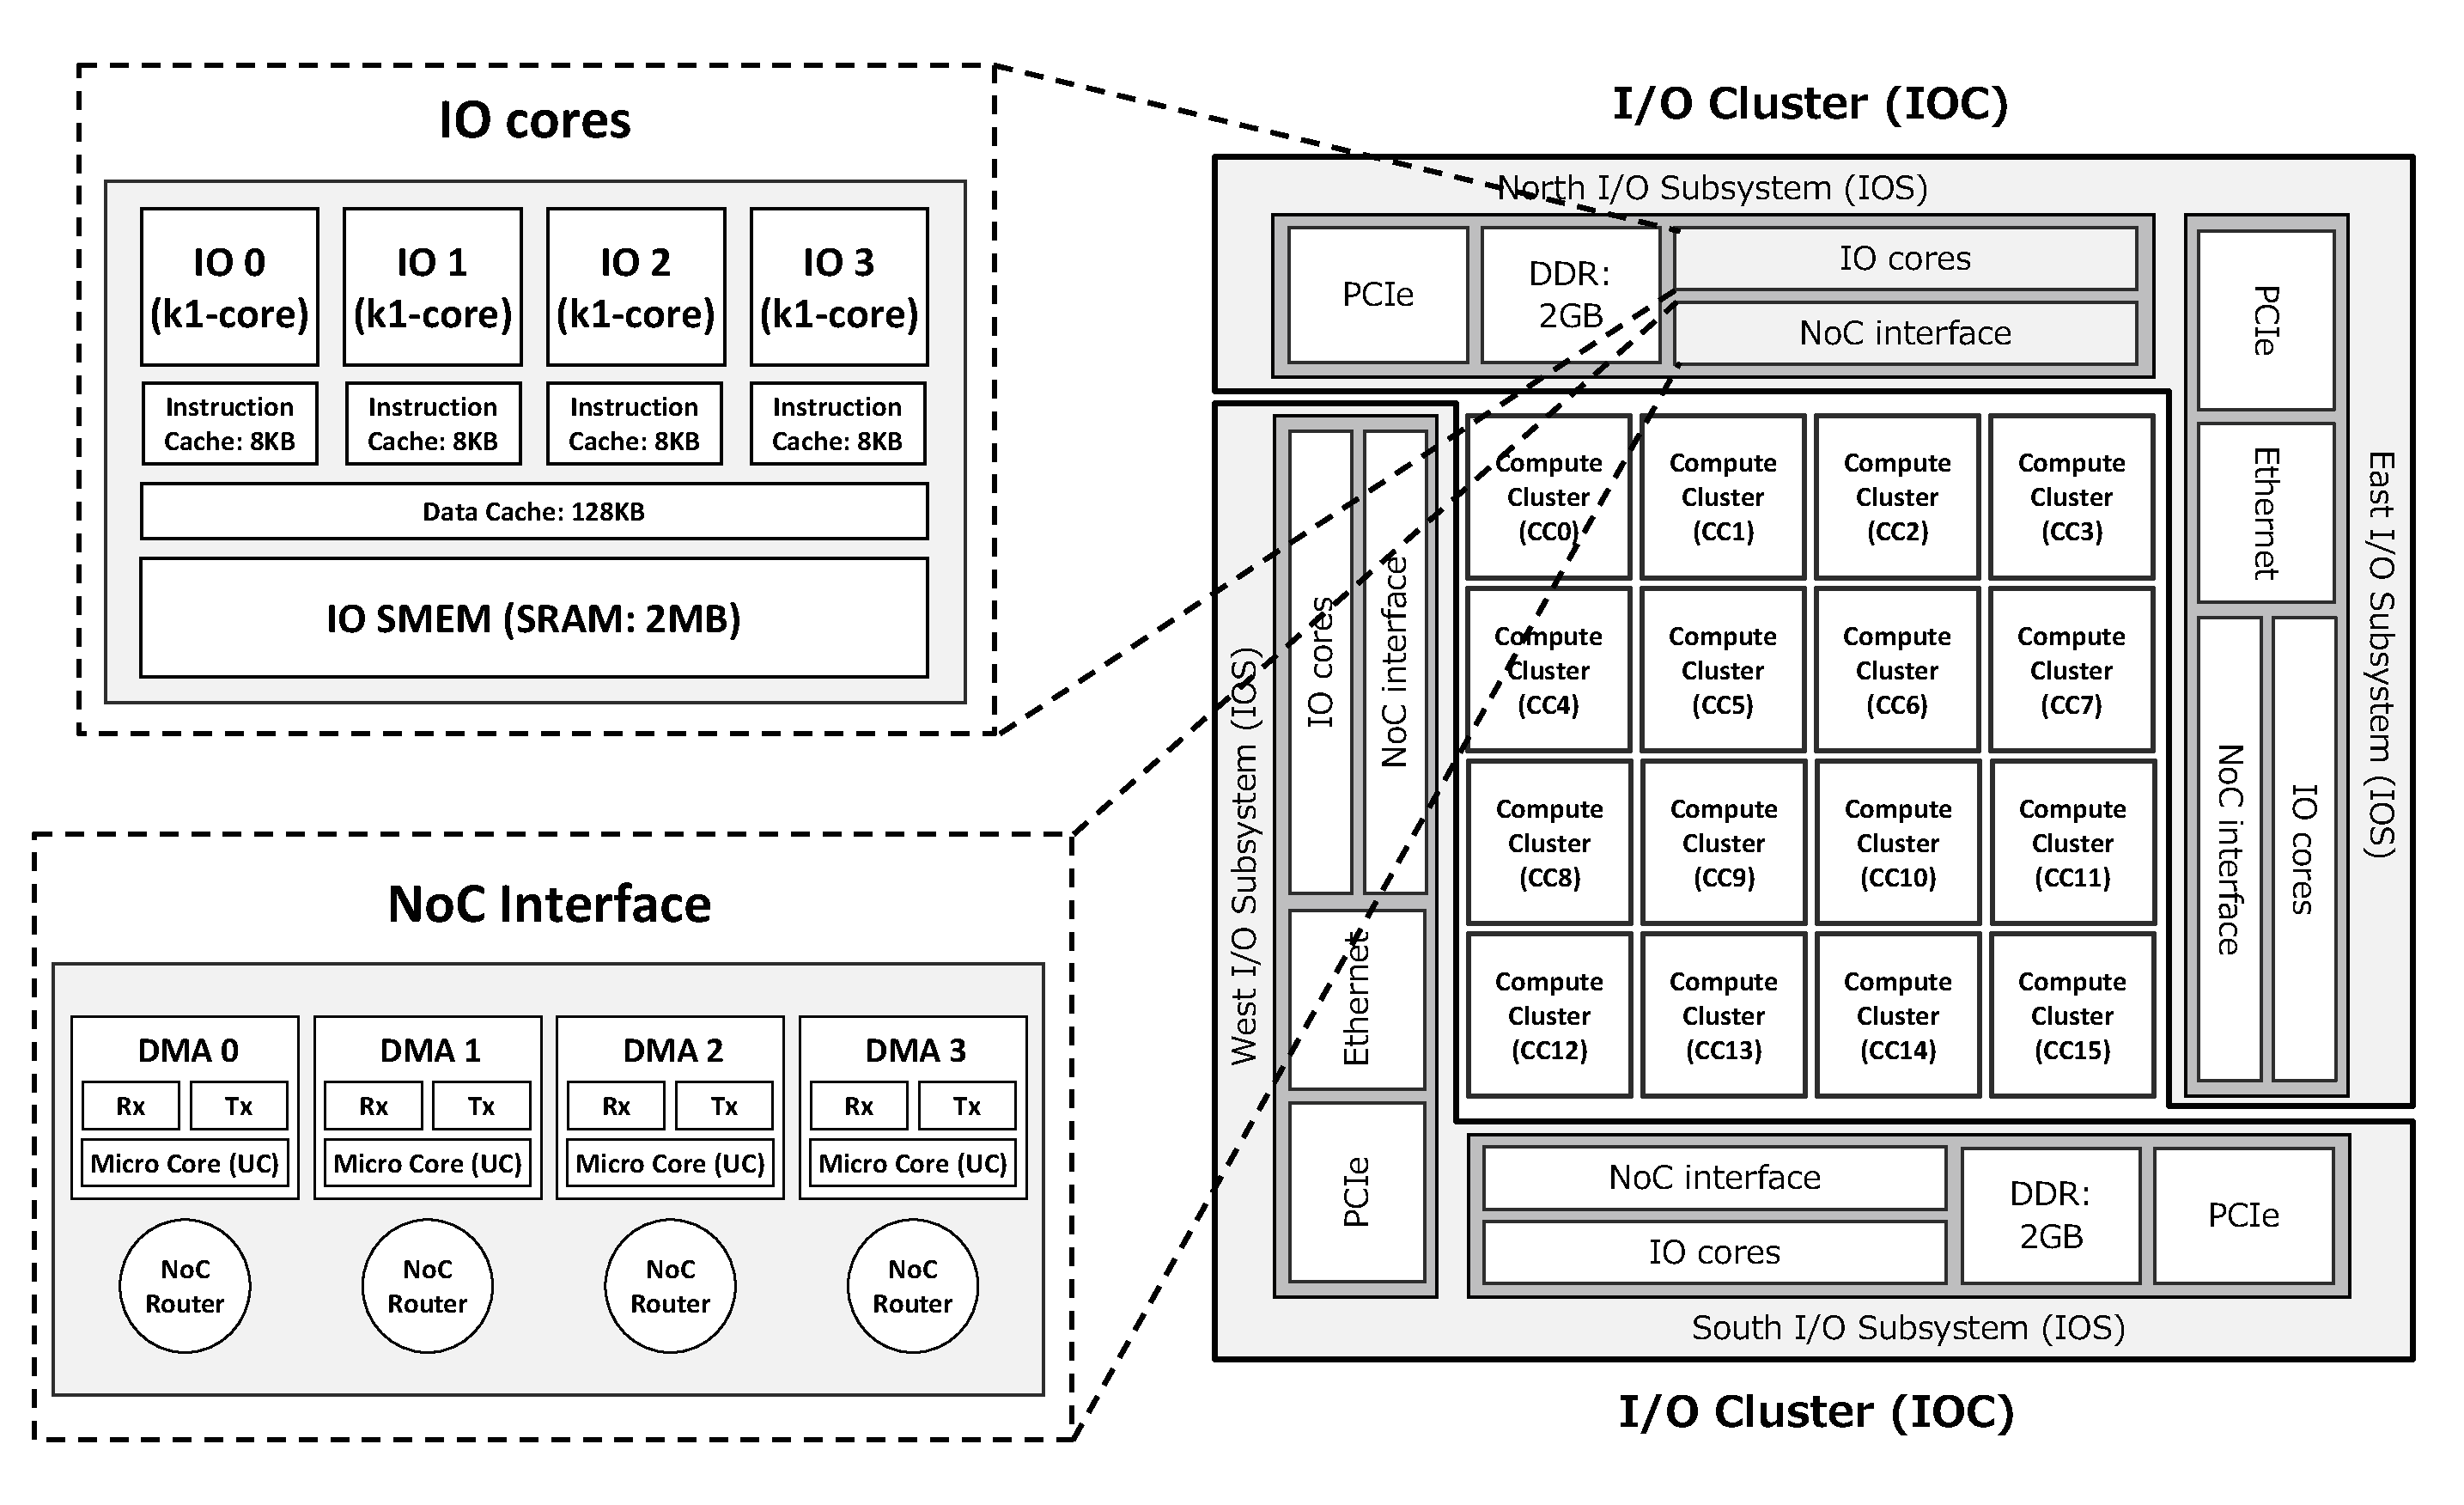
\includegraphics[width=1.0\linewidth]{../figure/mppa_architecture_brief.eps}
  \caption{\label{fig:mppa_architecture}
    An overview of the architecture of the Kalray MPPA-256 Bostan.}
\end{figure}

\begin{figure}[htbp]
  \centering
  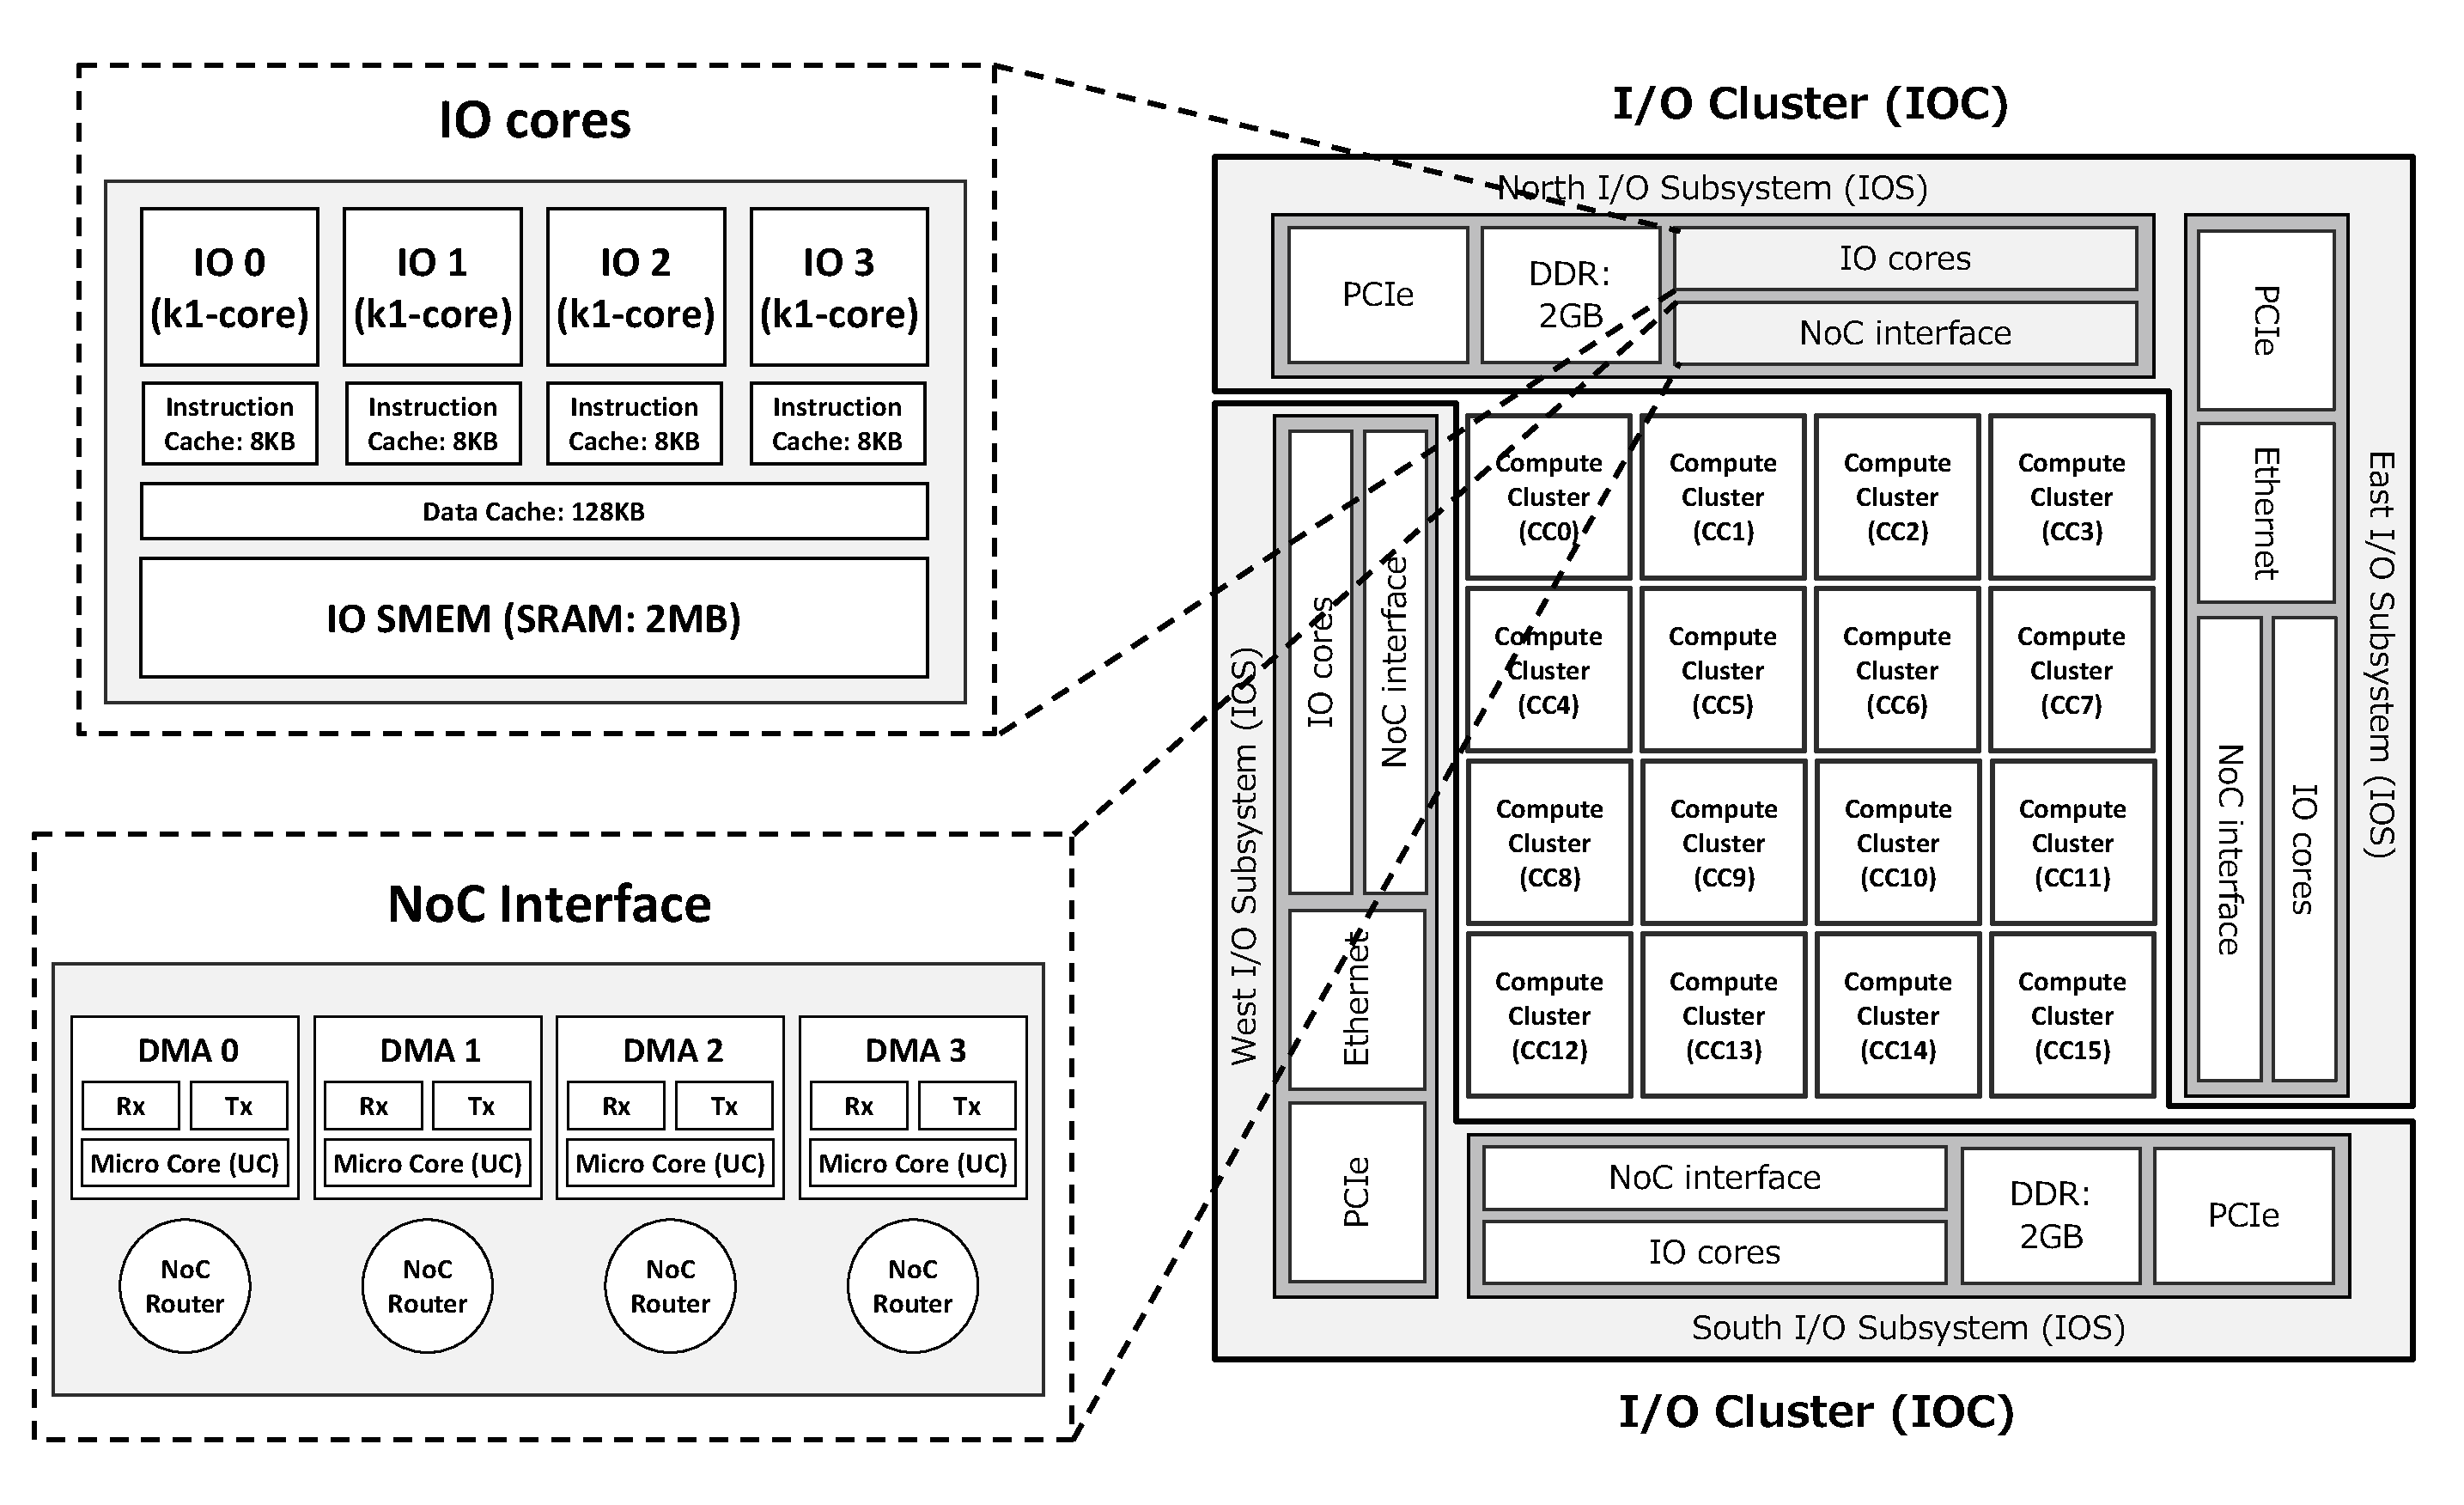
\includegraphics[width=1.0\linewidth]{../figure/mppa_architecture_brief.eps}
  \caption{\label{fig:mppa_architecture}
    An overview of the architecture of the Kalray MPPA-256 Bostan.}
\end{figure}

This section presents the system model used throughout the work.
The many-core model of Kalray MPPA-256 Bostan is considered.
First, a hardware model is introduced in Section \ref{sec:hardware_model}, followed by a software model in Section \ref{sec:software_model}.

% \begin{figure}[htbp]
%   \tabcolsep = 0.5mm              % side-margin in column
%   \begin{tabular}{cc}
%     \begin{minipage}[htbp]{0.49\textwidth}
%       \centering
%       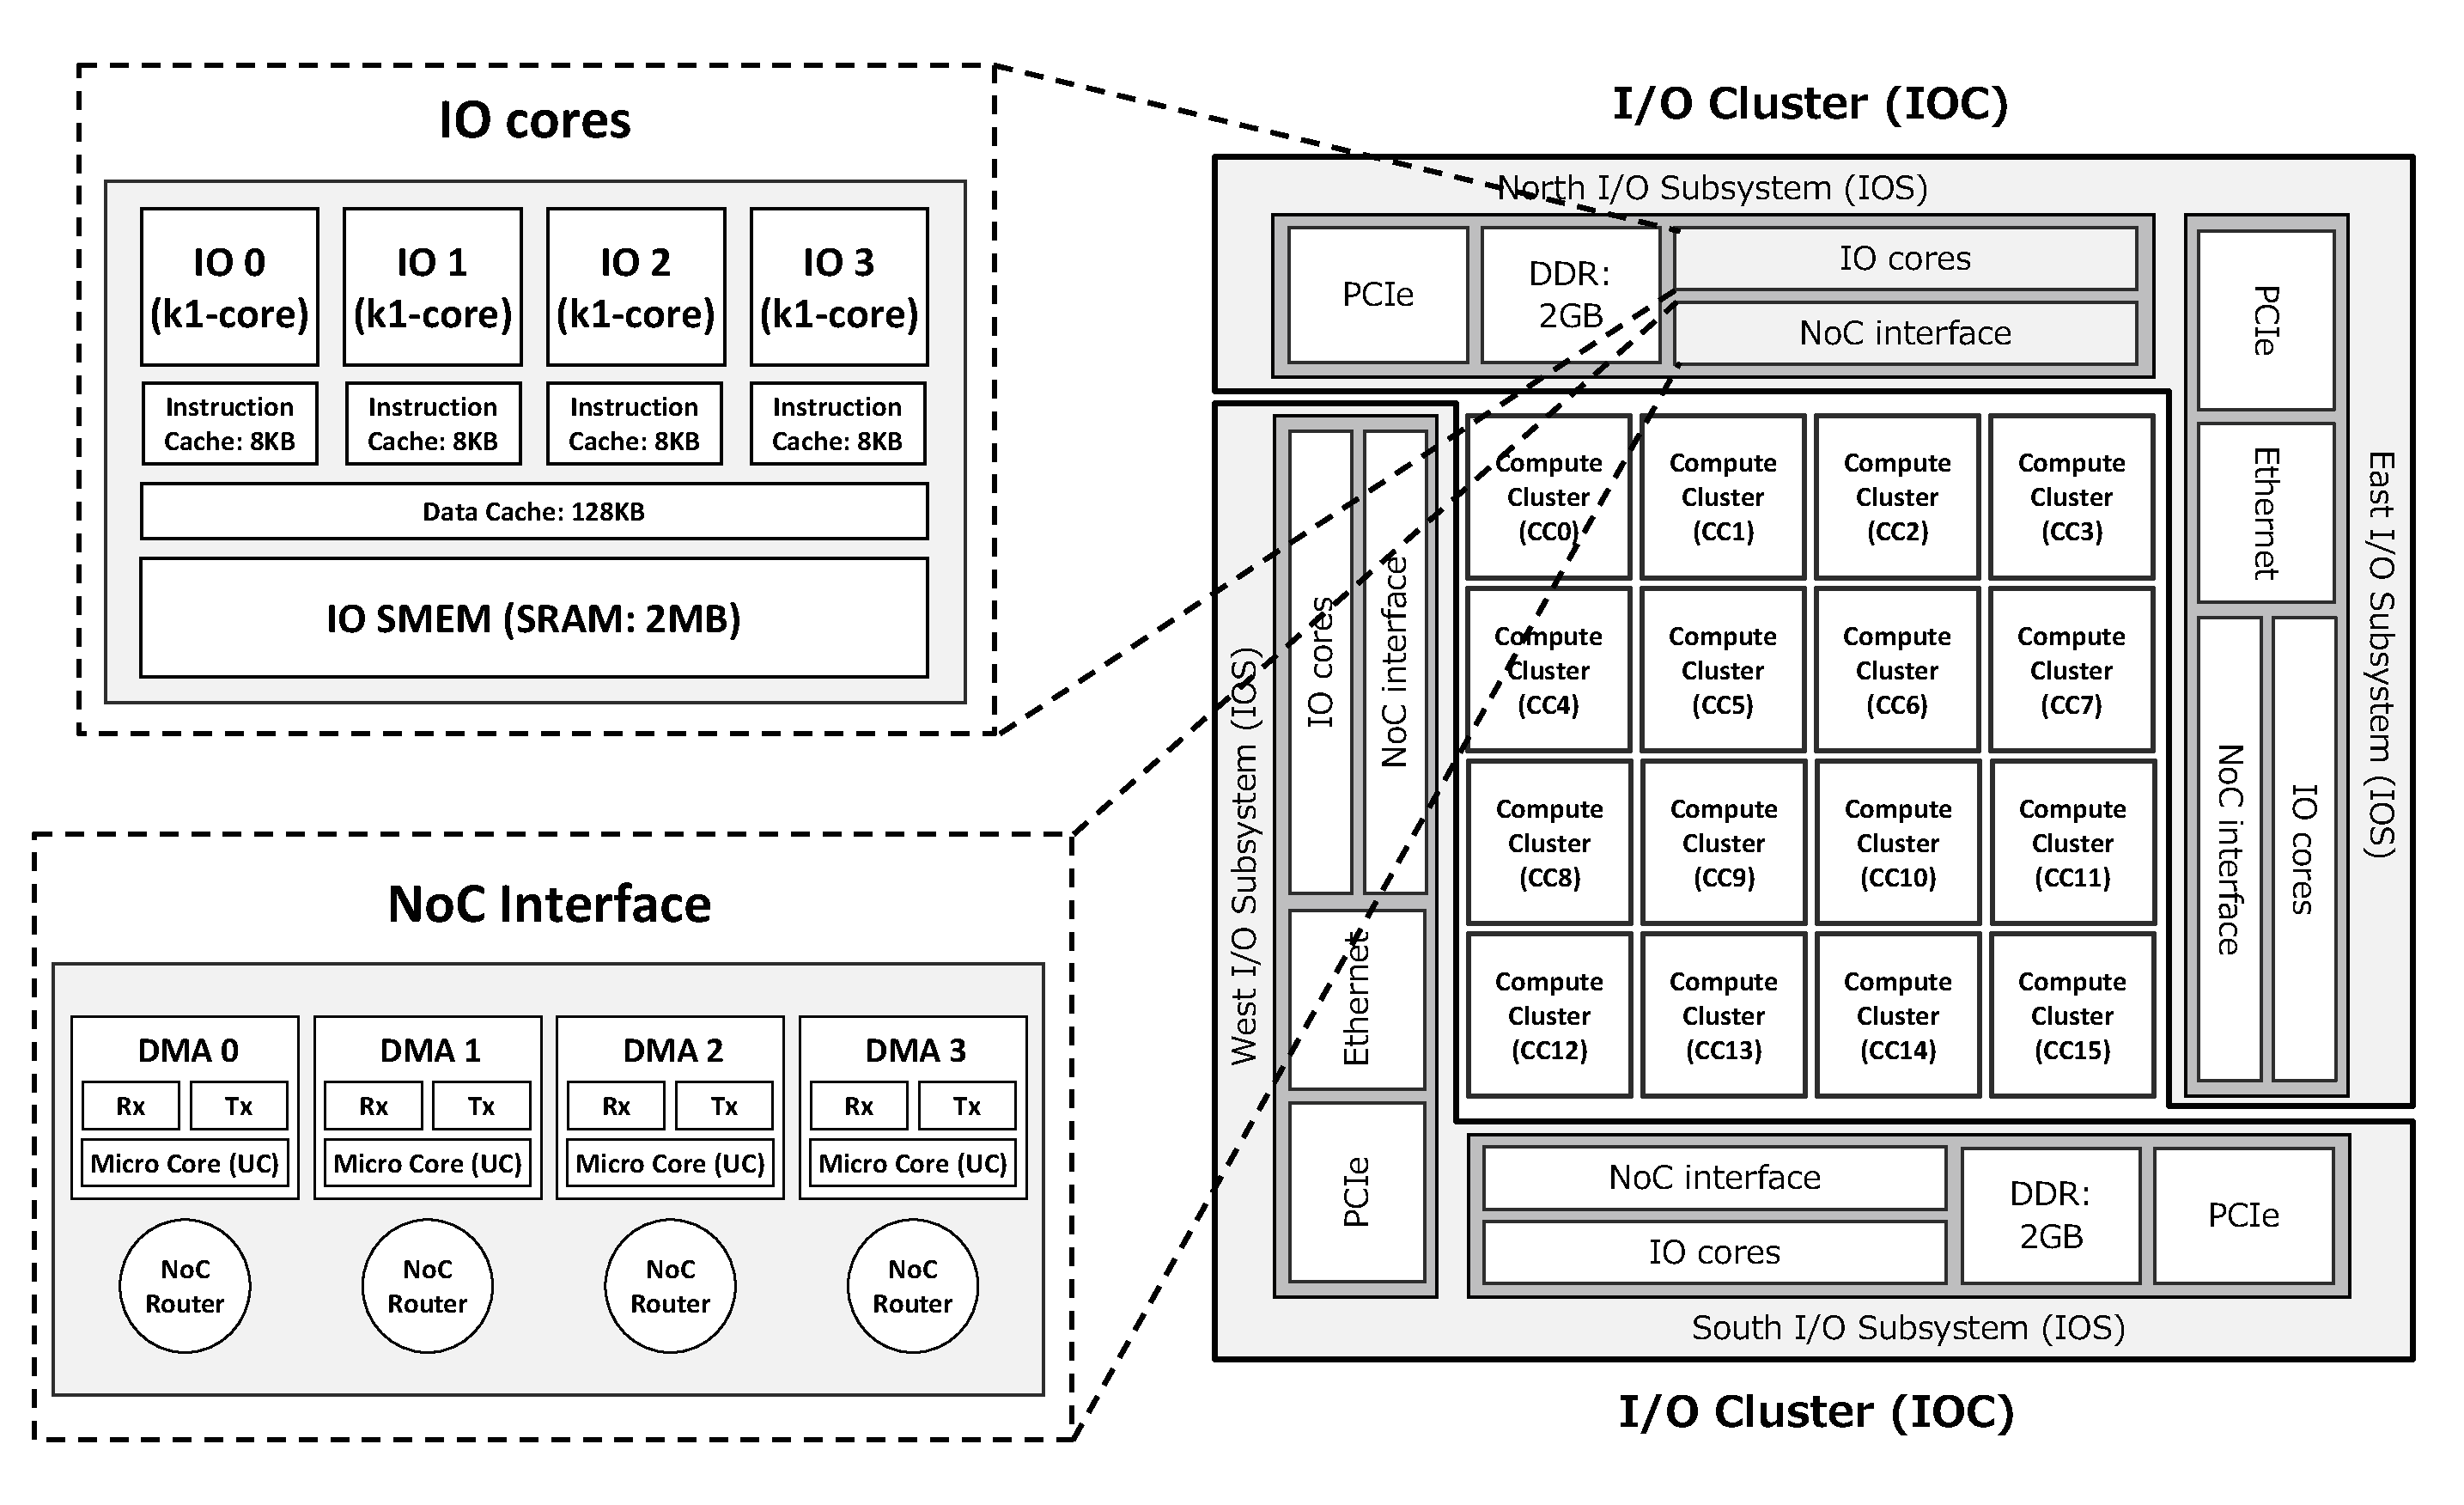
\includegraphics[width=1.0\linewidth]{../figure/mppa_architecture_brief.eps}
%       \caption{\label{fig:mppa_architecture}
%         An overview of the architecture of the Kalray MPPA-256 Bostan.}
%     \end{minipage}   
%     &
%     % \setcounter{figure}{11}
%     \begin{minipage}[htbp]{0.49\textwidth}
%       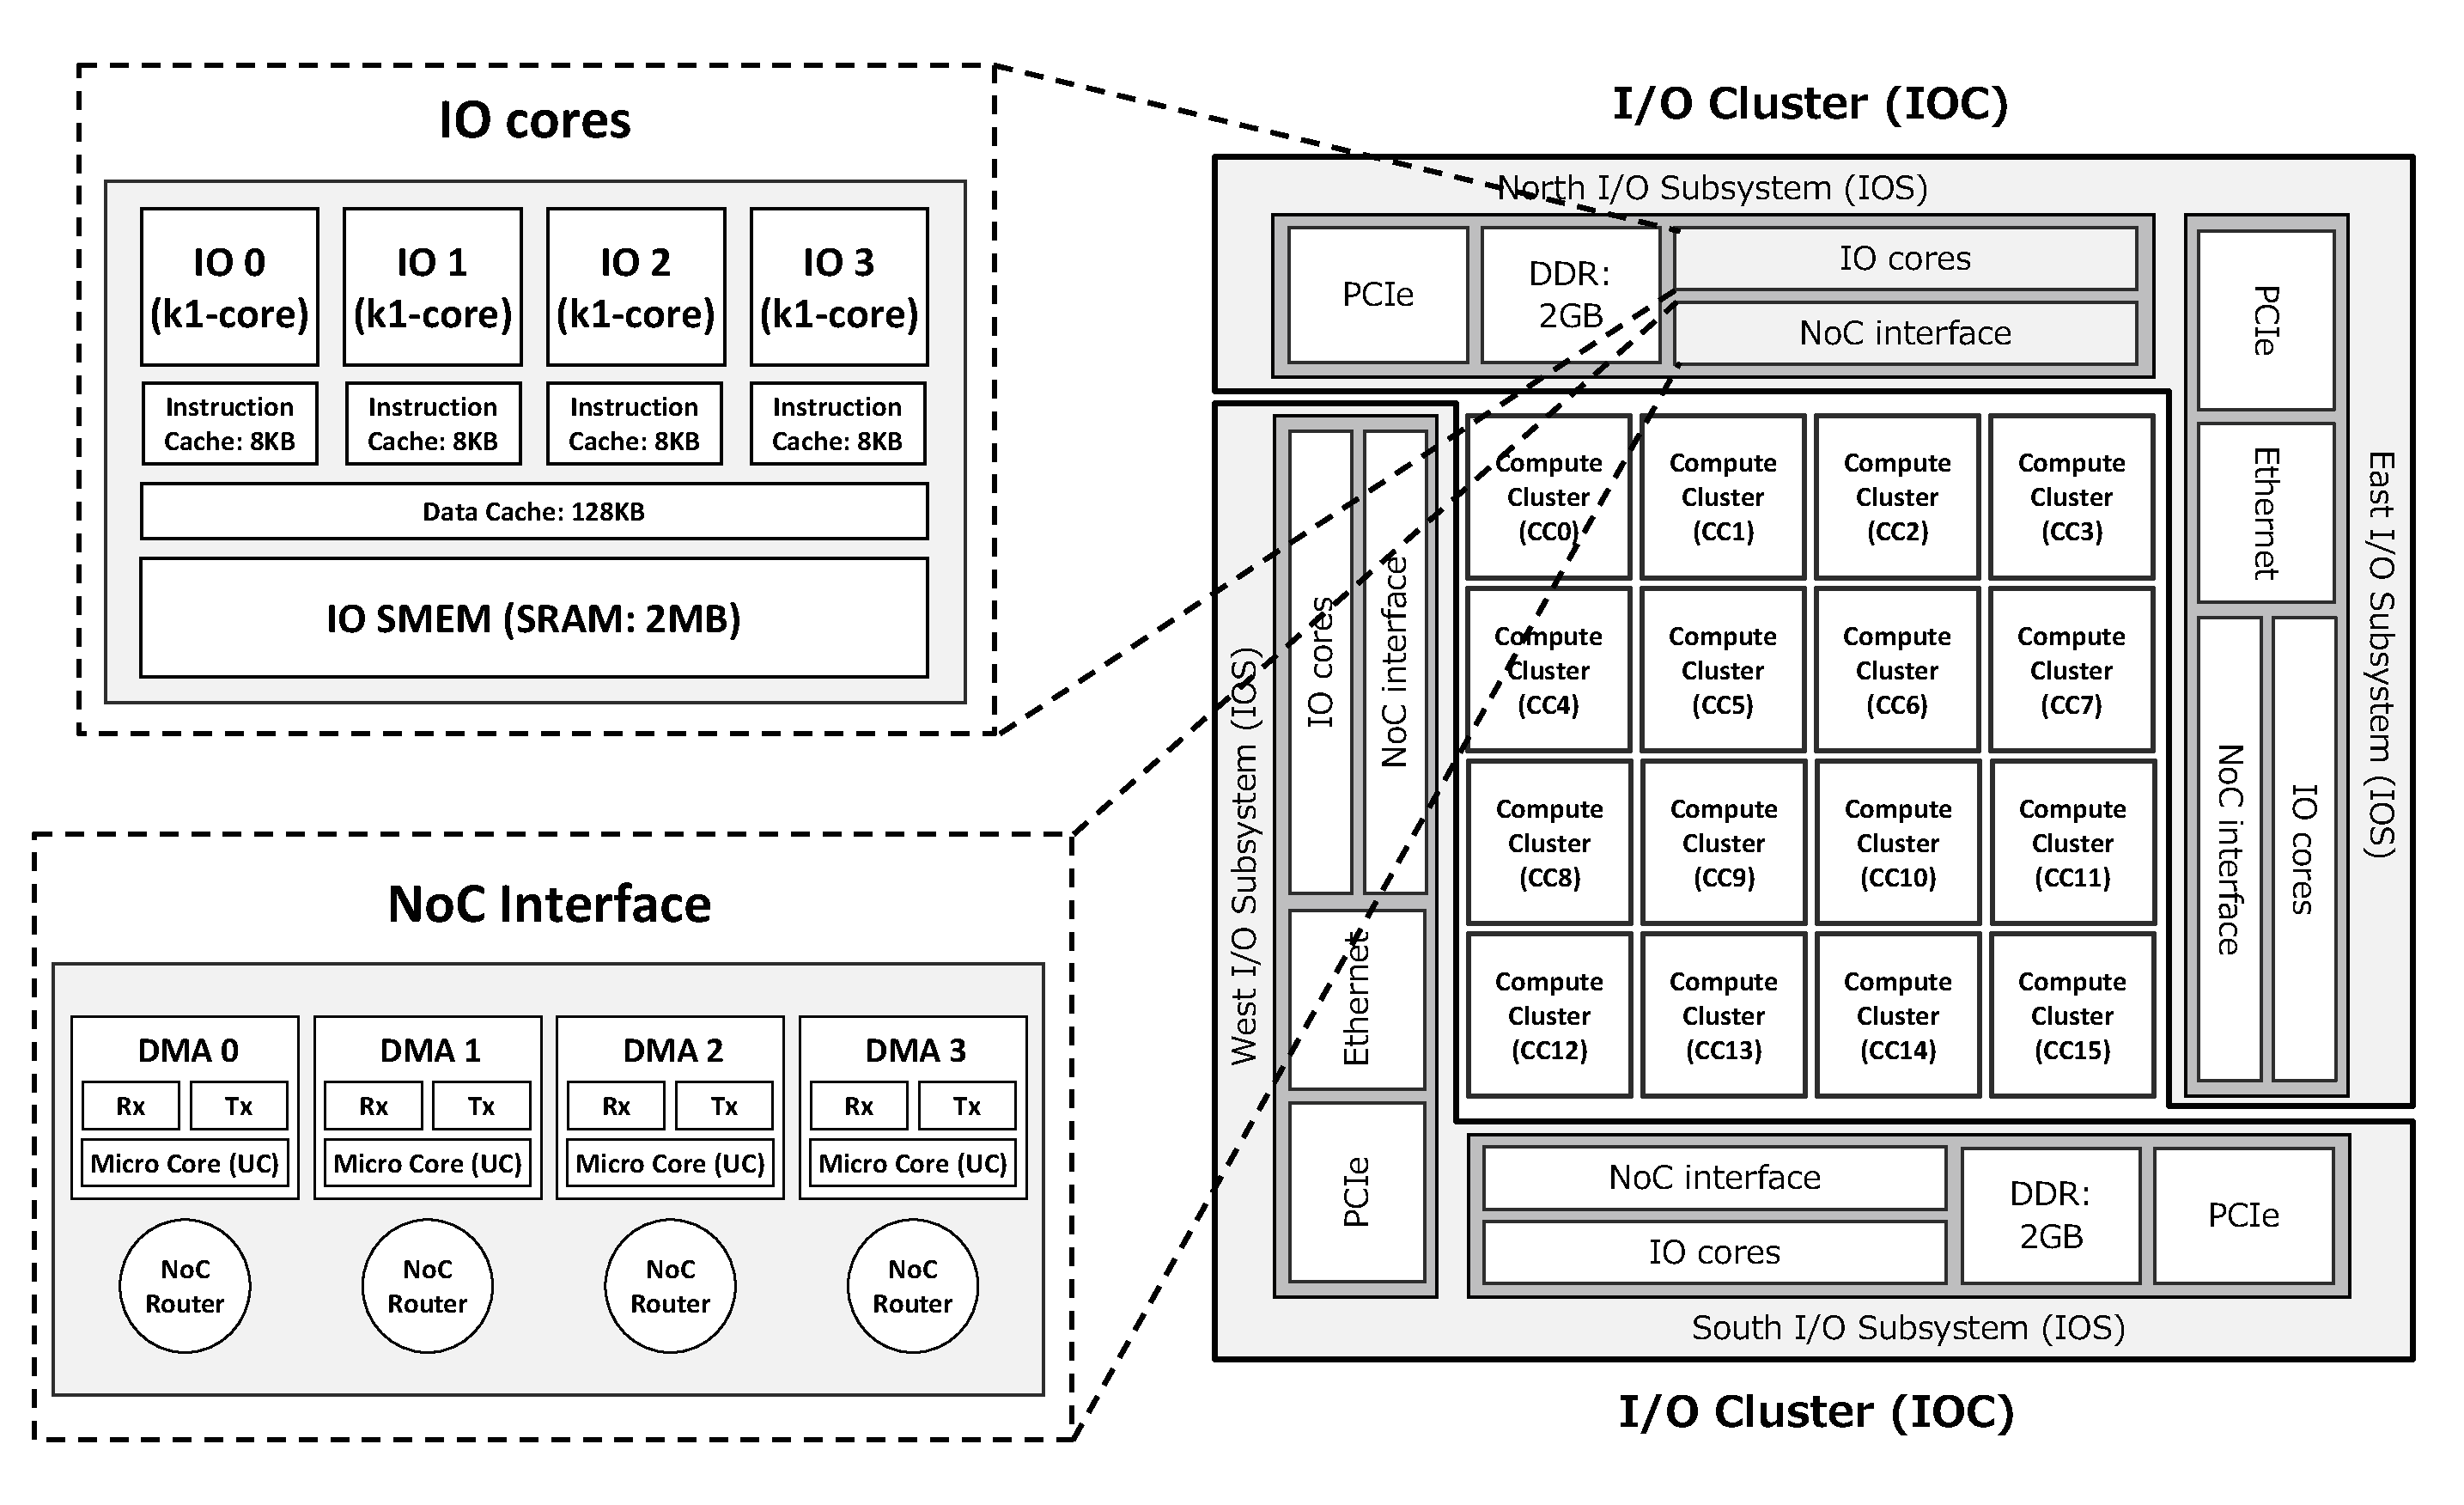
\includegraphics[width=1.0\linewidth]{../figure/mppa_architecture_brief.eps}
%       \caption{\label{fig:mppa_architecture}
%         An overview of the architecture of the Kalray MPPA-256 Bostan.}
%     \end{minipage}
%   \end{tabular}
% \end{figure} 


\section{Hardware Model}
\label{sec:hardware_model}
The MPPA-256 processor is based on an array of computing clusters (CCs) and I/O subsystems (IOSs) that are connected to NoC nodes with a toroidal two-dimensional topology 
(as shown in Figs. \ref{fig:mppa_architecture}, \ref{fig:cc_architecture} and \ref{fig:noc_map}).
The MPPA many-core chip integrates 16 CCs and 4 IOSs on NoC.
The architecture of Kalray MPPA-256 is presented in this section.

\section{I/O Subsystems (IOS)}
\label{sec:ios}
MPPA-256 contains the following four IOSs: North, South, East, and West.
The North and South IOSs are connected to a DDR interface and an eight-lane PCIe controller.
The East and West IOSs are connected to a quad 10 Gb/s Ethernet controller.
Two pairs of IOSs organize two I/O clusters (IOCs), as shown in Fig. \ref{fig:mppa_architecture}.
Each IOS consists of quad IO cores and a NoC interface.

\begin{itemize}
  \setlength{\leftskip}{-5mm}    
  \item \textbf{IO Cores}: IO cores are connected to a 16-bank parallel shared memory with a total capacity (IO SMEM) of 2 MB, as shown in Fig. \ref{fig:mppa_architecture}.
  The four IO cores have their own instruction cache 8-way associative corresponding to 32 ($8 \times 4$) KB and share a data cache 8-way with 128 KB and external DDR access.
  The sharing of the data cache of 128 KB allows coherency between the IO cores.
  Additionally, IO cores operate controllers for PCIe, Ethernet, \comment{1-11}and other I/O devices.
  They operate the local peripherals, including NoC interfaces with DMA.
  It is also possible to conduct an application run on the IO cores.
  
  \item \textbf{NoC Interface}: The NoC interface contains four DMA engines (DMA1-4) and four NoC routers, as shown in Fig. \ref{fig:mppa_architecture}, and the IOS DMA engine manages transfers between the IO SMEM, IOS DDR, and IOS peripherals (e.g., PCIe interface and Ethernet controllers).
  The DMA engine transfers data between routers via NoC through NoC routers and has the following three NoC interfaces: a receive (Rx) interface, a transmit (Tx) interface, and a microcore (UC).
  The UC is a fine-grained multithreaded engine that can be programmed to set threads sending data with a Tx interface.
  The UC can extract data from memory by using a programmed pattern and send the data on the NoC.
  After the UC is initiated, this continues in an autonomous fashion without using a processing element (PE) and an IO core.
\end{itemize}
% \begin{figure}[htbp]
%   \centering
%   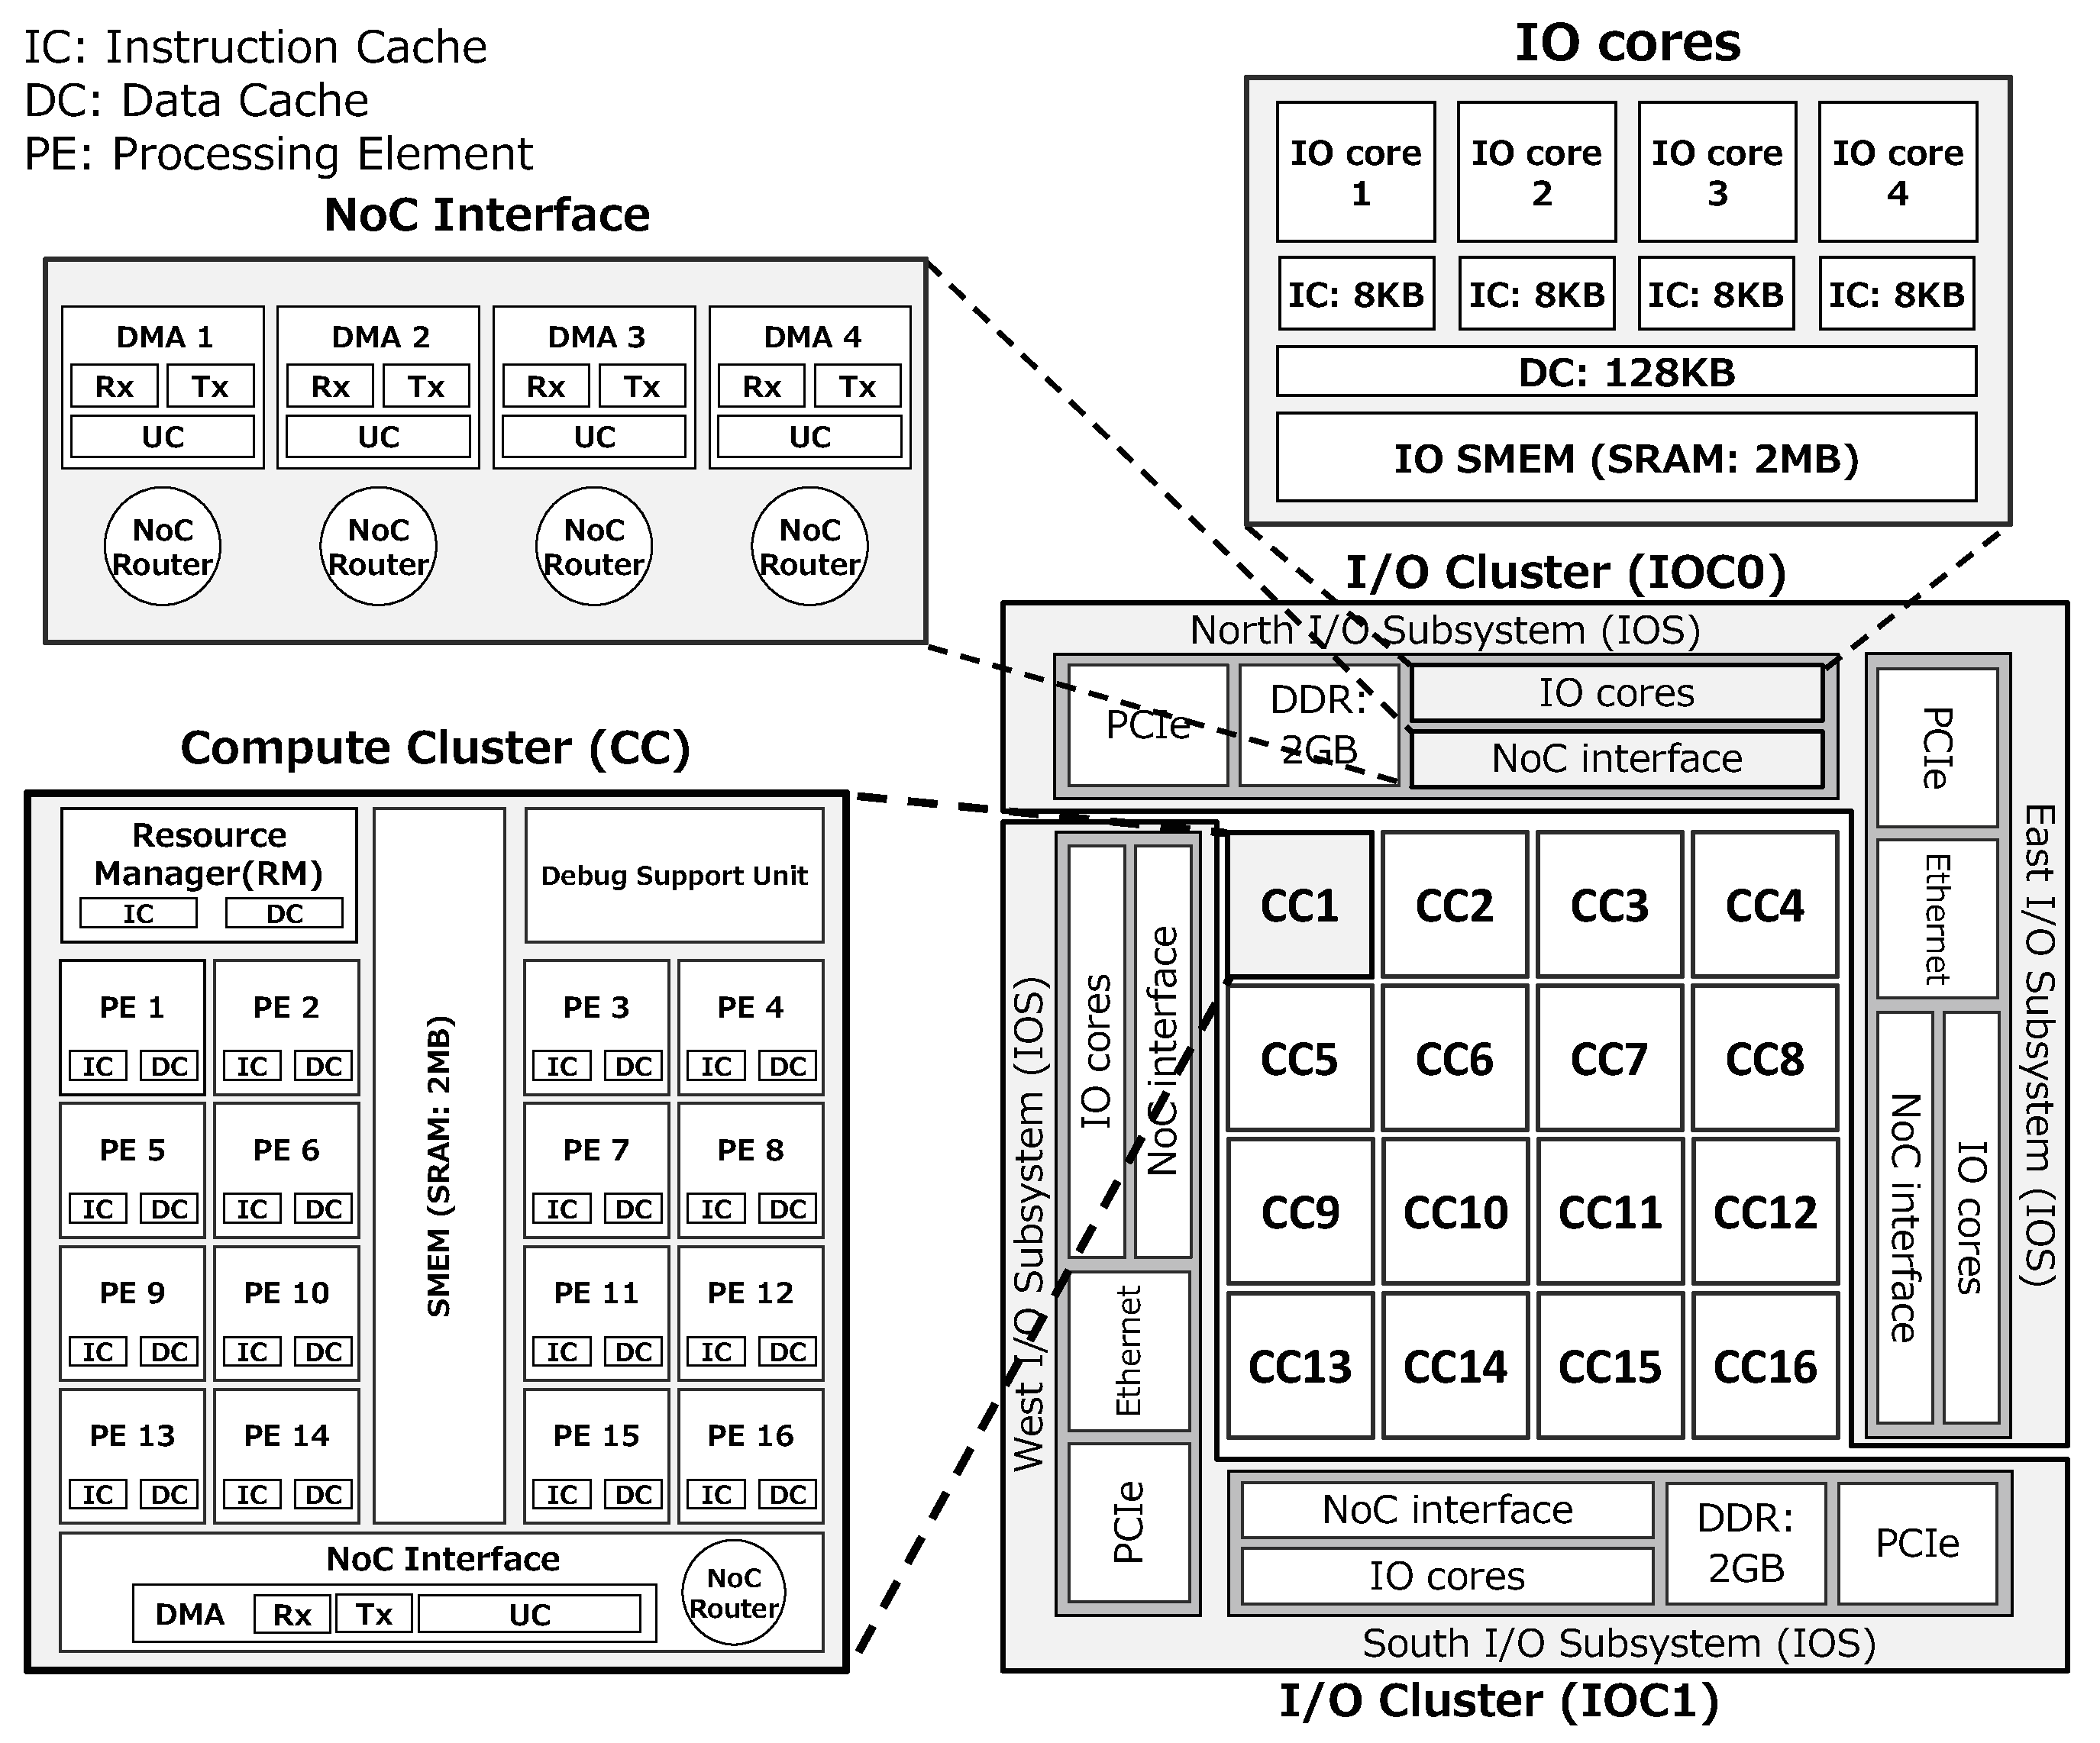
\includegraphics[width=1.0\linewidth]{../figure/mppa_architecture.eps}
%       \caption{\label{fig:mppa_architecture}
%     An overview of the architecture of the Kalray MPPA-256 Bostan.}
%   \end{figure}

\section{Compute Clusters (CCs)}
\label{sec:cc}
In MPPA-256, the 16 inner nodes of the NoC correspond to the CCs.
Fig. \ref{fig:cc_architecture} illustrates the architecture of each CC.

\begin{itemize}
  \setlength{\leftskip}{-5mm}    
  \item \textbf{PEs and an RM}:
  \comment{2-3}
  In a CC, 16 PEs and an RM share 2 MB cluster local memory (SMEM), so that 17 k1-cores (a PE or the RM) share 2 MB SMEM.
  % The capacity of each SMEM bank is 128 KB.
  Users use the PEs primarily for parallel processing.
  Developers spawn computing threads on PEs.
  The PEs and an RM in the CC correspond to the Kalray-1 cores, which implement a 32-bit 5-issue Very Long Instruction Word architecture with 600 or 800 MHz.
  Each core is fitted with its own instruction and data caches.
  Each cache is 2-way associative with a capacity of 8 KB.
  Note that these caches do not guarantee cache coherency.
  
  \item \textbf{A Debug Support Unit and a NoC Interface}:
  In addition to PEs and an RM, bus masters on the SMEM correspond to a Debug Support Unit and a DMA engine in a NoC interface.
  A DMA engine and a NoC router are laid out in a NoC interface.
  The CC DMA engine also has the following three interfaces: an Rx, a Tx, and a UC. 
  The CC DMA engine is instantiated in every cluster and connected to the SMEM.
\end{itemize}
% \begin{figure}[htbp]
%   \centering
%   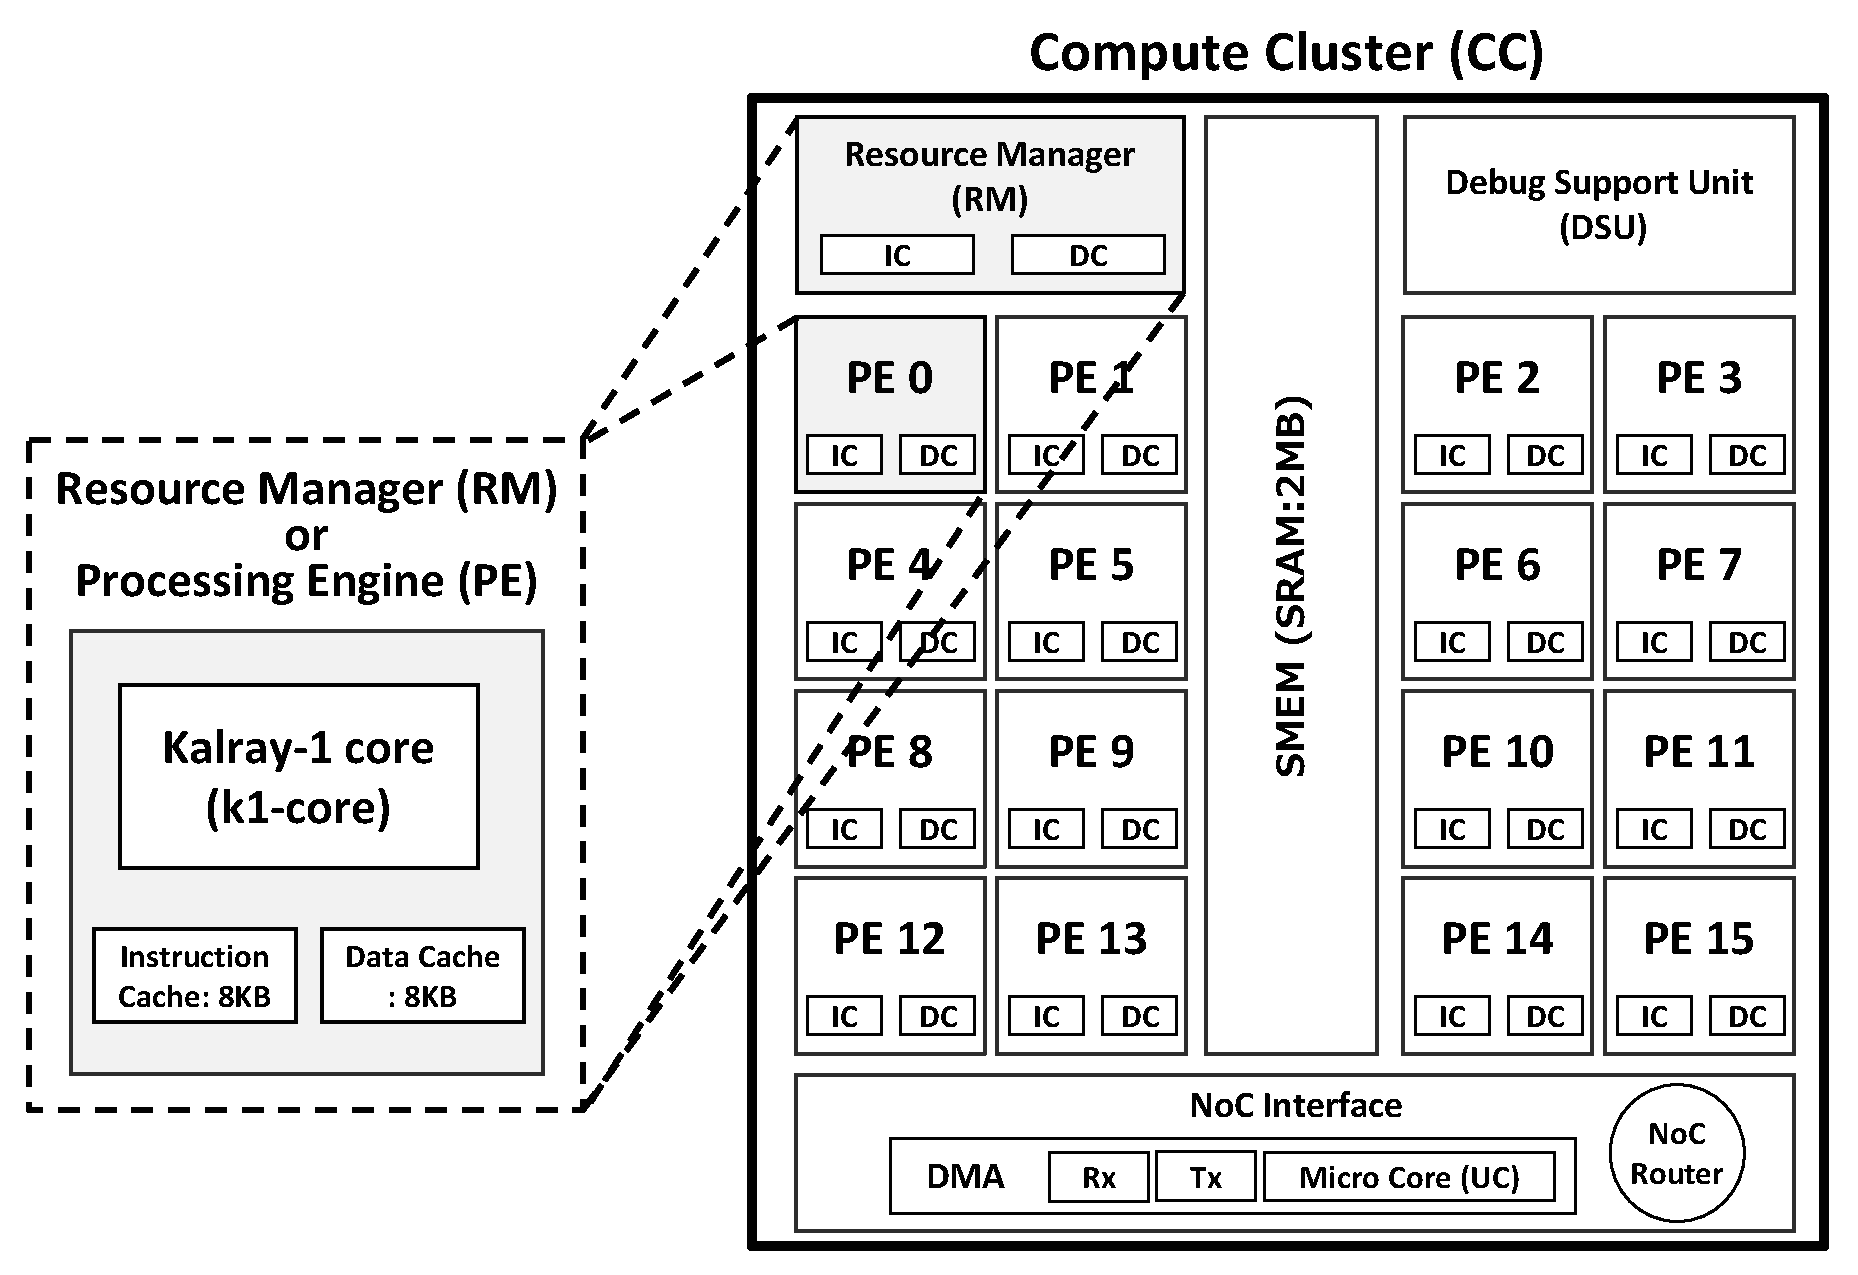
\includegraphics[width=1.0\linewidth]{../figure/cc_architecture.eps}
%   \caption{\label{fig:cc_architecture}
%     Compute Cluster architecture.}
% \end{figure}

\section{Network-on-Chip (NoC)}
\label{sec:noc}

\begin{figure}[htbp]
  \centering
  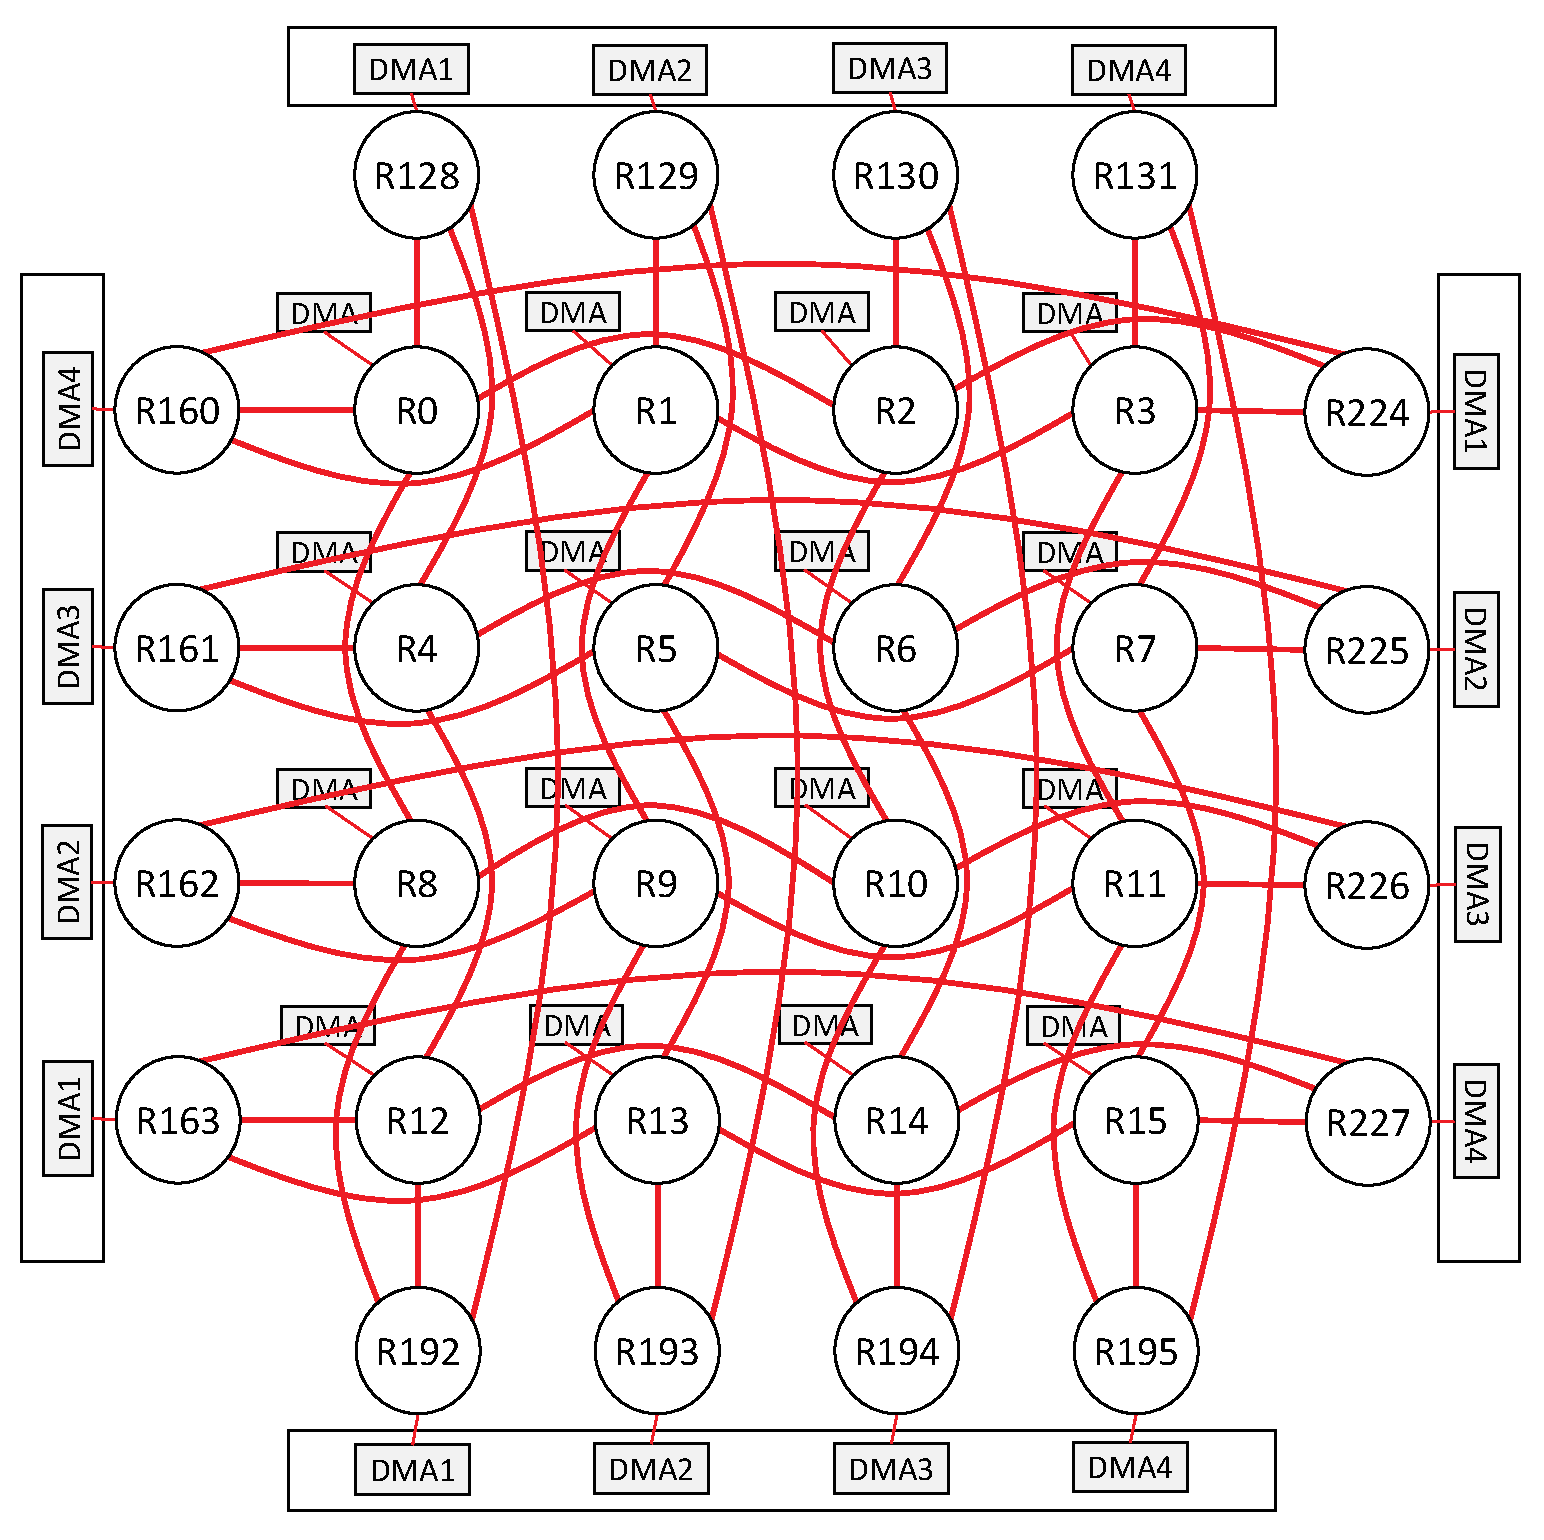
\includegraphics[width=0.9\linewidth]{../figure/noc_map.eps}
      \caption{\label{fig:noc_map}
    NoC connections (both D-NoC and C-NoC).}
\end{figure}

The 16 CCs and the four IOSs are connected by NoC as shown in Fig. \ref{fig:noc_map}.
Furthermore, NoC is constructed \comment{1-12} as the bus network and has routers on each node.

\begin{itemize}
  \setlength{\leftskip}{-5mm}
  \item \textbf{Bus Network}:
  A bus network connects nodes (CCs and IOSs) with torus topology \cite{dally2001route}, which \comment{1-13} involves a low average number of hops when compared to mesh topology \cite{vangal200780}, \cite{taylor2002raw}.
  The network is actually composed of the following two parallel NoCs with bidirectional links (denoted by red lines in Fig. \ref{fig:noc_map}):
  the data NoC (D-NoC) that is optimized for bulk data transfers and the control NoC (C-NoC) that is optimized for small messages at low latency.
  The NoC is implemented with wormhole switching and source routing.
  Data is packaged in variable length packets that are broken into small pieces called flits (flow control digits).
  The NoC traffic is segmented into packets, with each packet including 1-4 header flits and 0-62 payload data flits.
  
  \item \textbf{NoC routers}:
  One node per CC and four nodes per I/O subsystem hold the following two routers of their own: a D-NoC router and a C-NoC router.
  Each RM or IO core on a NoC node is associated with the two aforementioned  NoC routers.
  Furthermore, DMA engines in a NoC interface on the CC/IOS send and receive flits through the D-NoC routers with the Rx interface, the Tx interface, and the UC.
  A mailbox component corresponds to the virtual interface for the C-NoC and enables one-to-one, N-to-one, or one-to-N low-latency synchronization.
  The NoC routers shown in Fig. \ref{fig:cc_architecture} illustrate nodes as R1-16, R128-131, R160-163, R224-227, and R192-195 in Fig. \ref{fig:noc_map}.
  % The NoC routers are illustrated as nodes in Fig. \ref{fig:noc_map}.
  For purposes of simplicity, D-NoC/C-NoC routers are illustrated with a NoC router.
  In both D-NoC and C-NoC, each network node (a CC or an IOS)  includes the following 5-link NoC routers:
  four duplexed links for North/East/West and South neighbors and a duplexed link for local address space attached to the NoC router.
  The NoC routers include FIFOs queuing flits for each direction.
  The data links are four bytes wide in each direction and operate at the CPU clock rates of 600 MHz or 800 MHz, with the result that each tile can transmit/receive a total of 2.4 GB/s or 3.2 GB/s, which is spread across the four directions (i.e., North, South, East, and West).
\end{itemize}  

\section{Software Model}
\label{sec:software_model}

\begin{figure}[htbp]
  \centering
  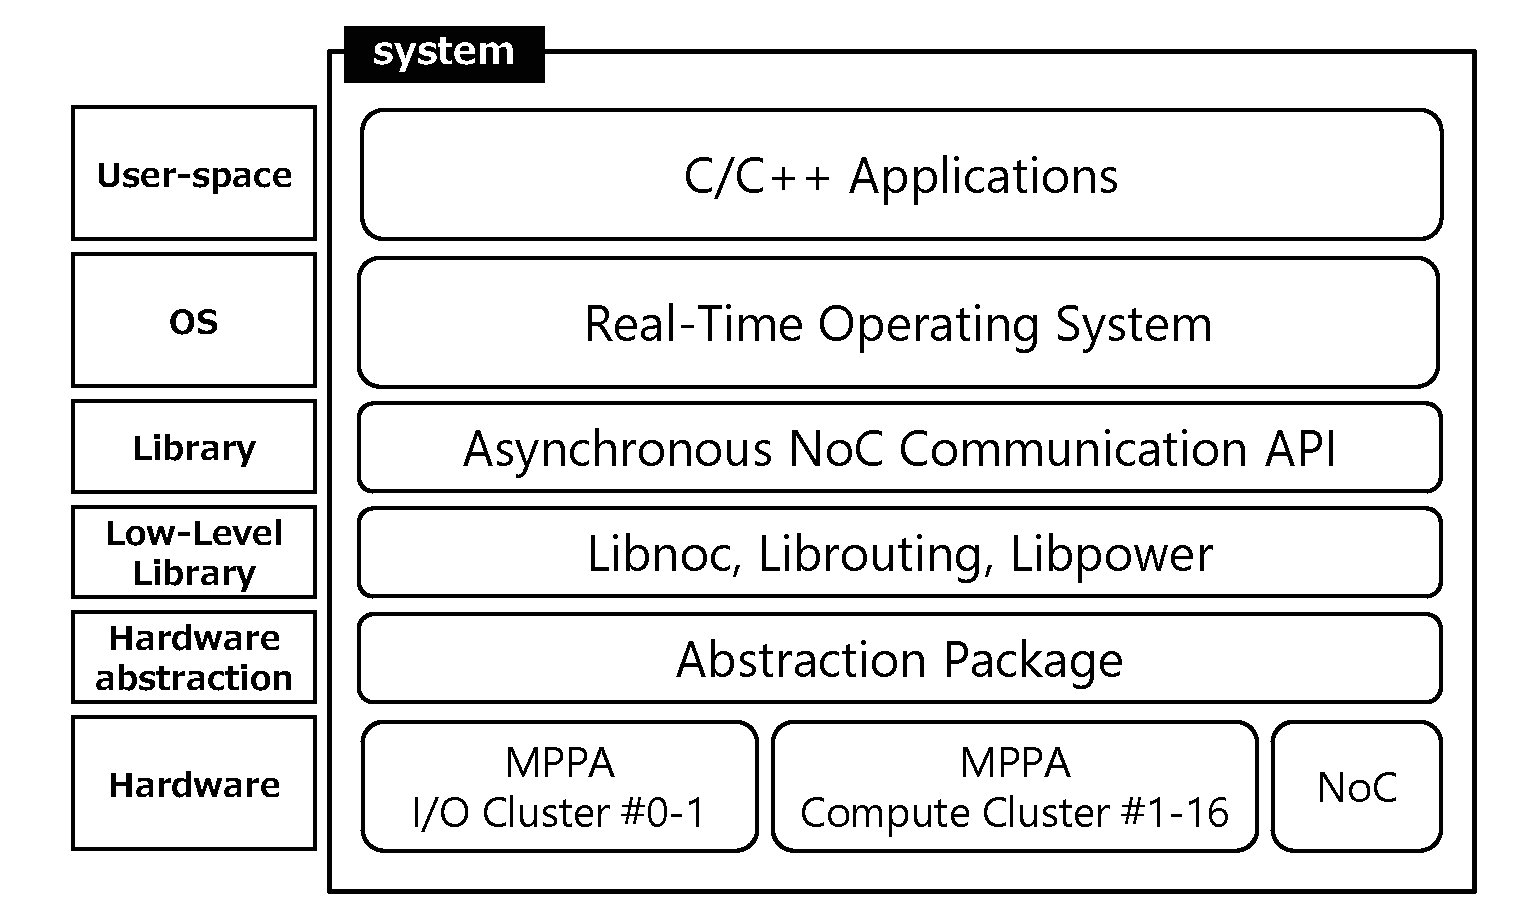
\includegraphics[width=0.8\linewidth]{../figure/softwarestack.eps}   
  \caption{\label{fig:software_stack}
    The software stack of Kalray MPPA-256.}     
\end{figure}

The software stack used for Kalray MPPA-256 is composed of a hardware abstraction layer, a low-level layer, an OS, and a user application.  
Fig. \ref{fig:software_stack} shows the software stack used for Kalray MPPA-256 in the present work.
The Kalray system is an extensible and scalable array of computing cores and memory.
With respect to the scalable computing array of the system, it is possible to map several programming models or runtimes such as Linux, a real-time operating system, POSIX API, OpenCL, and OpenMP.
Each layer is described in detail.

In the hardware abstraction layer, an abstraction package abstracts hardware of a CC, an IOS, and NoC.
\comment{1-15} % The abstraction package serves as a system that does not provide any services.
The hardware abstraction is responsible for partitioning hardware resources and controlling access to the resources from the user-space operating system libraries.
\comment{1-16} 
% Additionally, the abstraction package retrieves resources allocated to a partition at any time.
The abstraction sets-up and controls interpartition communications as a virtual machine abstraction layer.
The hardware abstraction runs on the dedicated RM core.
All the services are provided commonly by an operating system (e.g., virtual memory and schedule) that must be provided by user-space libraries.
% Consequently, each runtime or operating system implements its own services that are optimized to specific needs.
% This is because each programming model or runtime involves different requirements.
A minimal kernel avoids wastage of resources and mismatched needs.

In a low-level library layer, the Kalray system also provides Libnoc and Librouting for handling NoC.
Additionally, NoC features such as routing and quality of service are set by the programmer.
Libnoc allows direct access to memory mapped registers for their configurations and uses.
This library is designed to cause minimum CPU overhead and also serves as a minimal abstraction for resource allocation.
% Librouting offers a minimal set of functions that can be used to route data between any clusters of the MPPA including unicast (one target) modes or multicast (multiple targets) modes.
Librouting offers a minimal set of functions that can be used to route data between any clusters of the MPPA.
Routing on the network is conducted statically with its own policy.
In addition, Libpower enables spawning and waiting for the end of execution of other clusters.

\comment{1-17}
% Routing on the torus network is statically conducted with its own policy.
% The Libpower enables spawning and waiting for the end of execution of a remote cluster.

Several operating systems support the abstraction package in the OS layer.
It is difficult for numerous cores such as MPPA to support previous operating systems for single/multicore(s) owing to problems involving parallelism and cache coherency \cite{Wentzlaff2009FOS}, \cite{schupbach2008embracing}.
Here, the following real-time operating systems (RTOSs) supporting MPPA are introduced:

\begin{itemize}
  \setlength{\leftskip}{-5mm}    
  \item \textbf{RTEMS}: Real-Time Executive for Multiprocessor Systems (RTEMS) is a full featured RTOS prepared for embedded platforms.
  RTEMS supports several APIs and standards, and most notably supports the POSIX API.
  The system provides a rich set of features, and an RTEMS application is mostly a regular C or C++ program that uses the POSIX API.
  \comment{1-18}
  RTEMS runs on the IOC except for the CC.
  
  \item \textbf{NodeOS}: On the CC, the MPPA cluster operating system utilizes a runtime called NodeOS.
  The OS addresses the need for a multicore OS to conform to the maximum possible extent to the standard POSIX API.
  The NodeOS enables a user code by using the POSIX API to run on PEs on the CC.
  First, NodeOS runtime starts on PE0 prior to calling the user main function.
  Subsequently, \texttt{pthread} is called on other PEs.
  
  \item \textbf{eMCOS}: On both CCs and IOSs, eMCOS provides minimal programming interfaces and libraries.
  Specifically, eMCOS is a real-time embedded operating system developed by eSOL (a Japanese supplier for RTOSs) and is the first commercially available many-core RTOS for use in embedded systems.
  The OS implements a distributed microkernel architecture.
  This compact microkernel is equipped with only minimal functions.
  The eMCOS enables applications to operate priority based message passing, local thread scheduling, and thread management on IOSs as well as CCs.
\end{itemize}

RTMES and NodeOS are provided by Kalray and eMCOS is released by eSOL.

\chapter{Evaluations}
\label{sec:evaluations}
First, this section involves examining two types of evaluations: a D-NoC data transfer evaluation in which latency characteristics of interfaces and memory type are explored and a matrix calculation evaluation that demonstrates the parallelization potential of the MPPA-256 and its memory access characteristics.
Subsequently, we conduct a practical self-driving application to examine the practicality of NUMA many cores.
% Finally, we arrange lessons learned from above evaluations.
The following evaluations are all conducted on real hardware boards with eMCOS.

\section{D-NoC Data Transfer}
\label{sec:dnoc_eval}

\subsection{Situations and Assumptions}
\label{sec:situations_and_assumptions}

\begin{figure}[htbp]
  \centering
  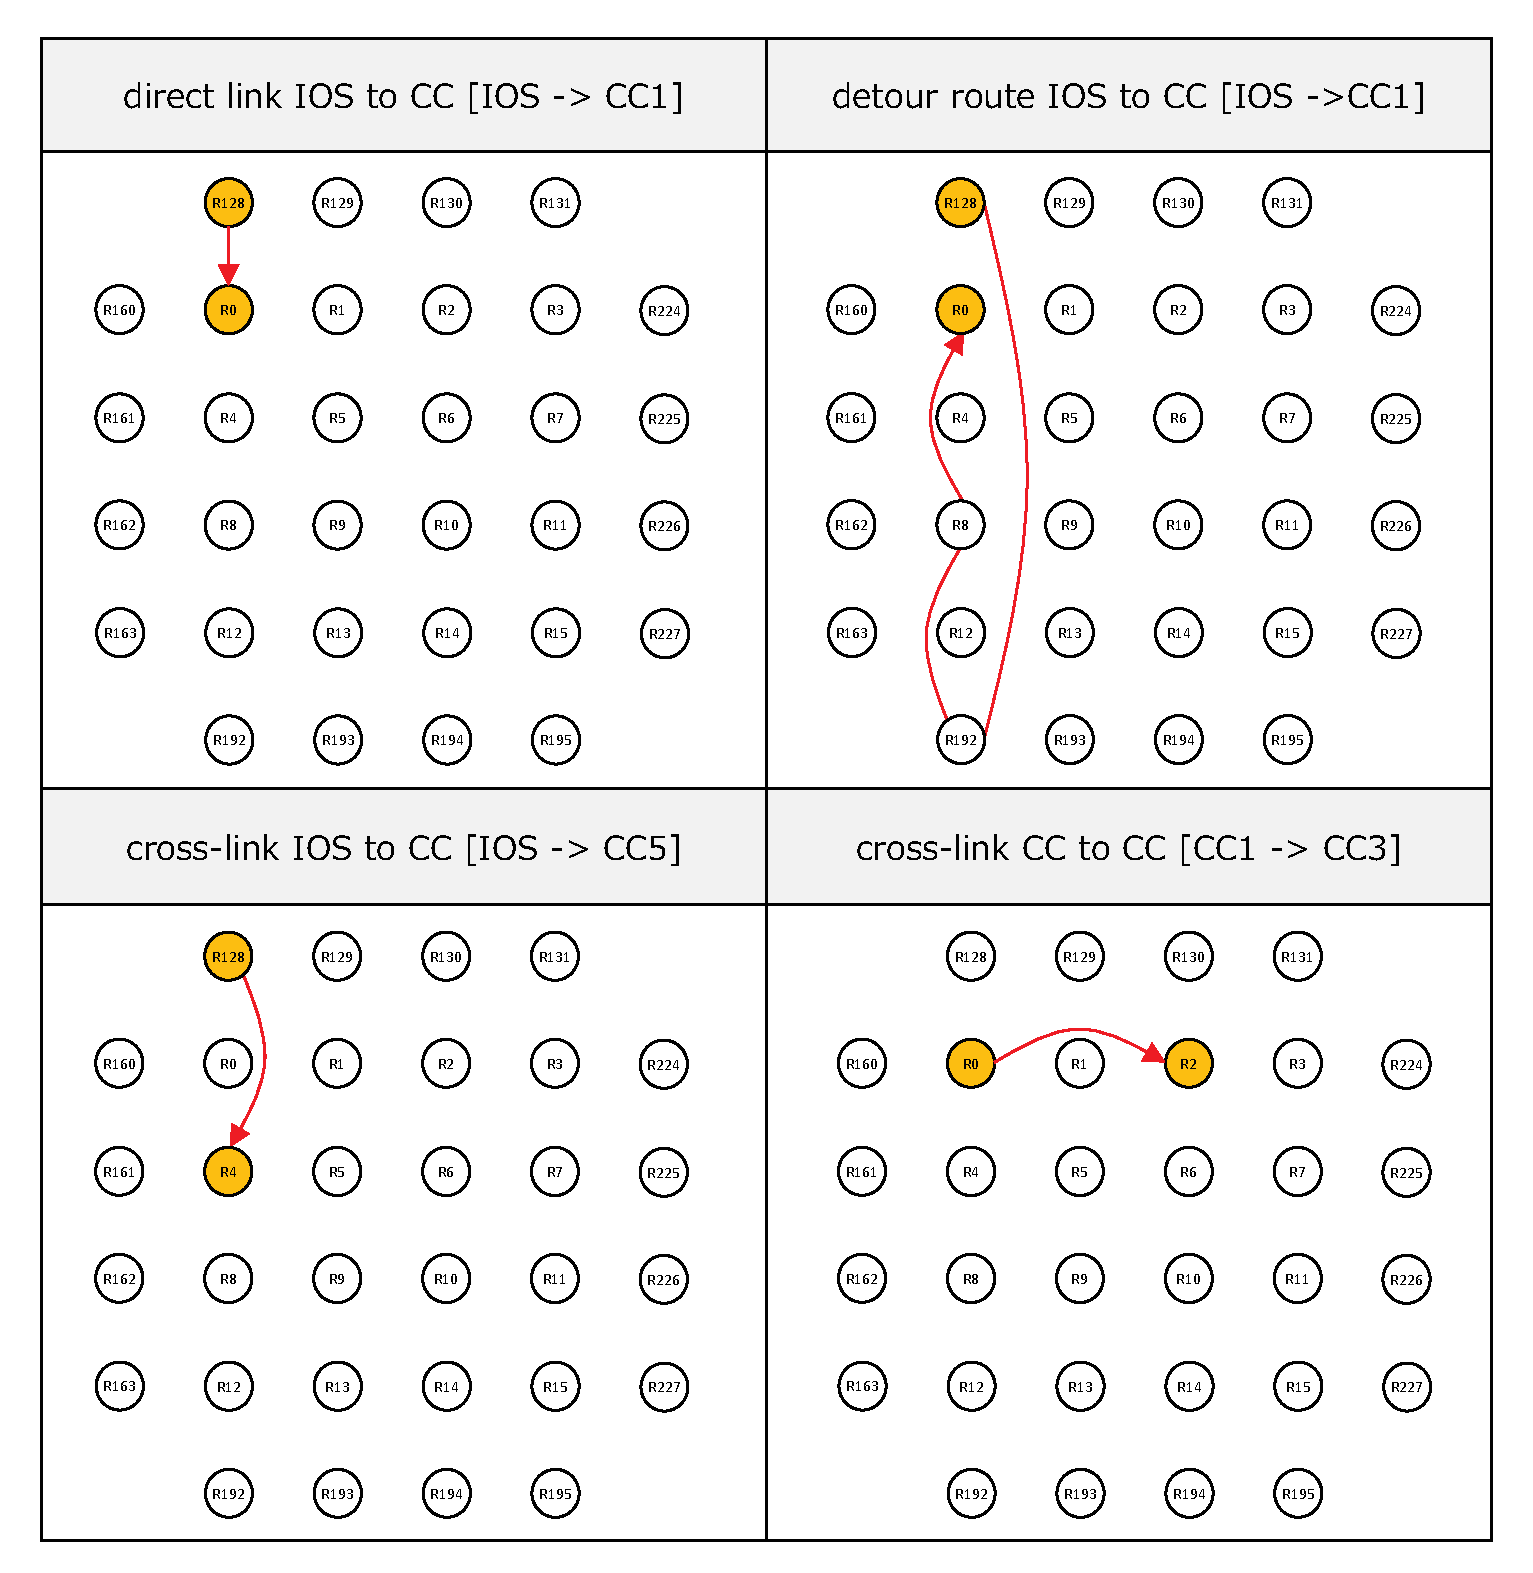
\includegraphics[width=0.8\linewidth]{../figure/noc_routes_old.eps}
      \caption{\label{fig:noc_routes}
    Four D-NoC routes used in the evaluation.}
\end{figure}

This evaluation involves clarifying end-to-end latency by considering the relation among interfaces (Tx or UC), routing on NoC, and memory type (DDR or SMEM).
This is achieved by preparing four routes as shown in Fig. \ref{fig:noc_routes}.
The routes on the D-NoC map (Fig. \ref{fig:noc_map}) contain various connections between routers, a direct link, a cross-link, and a flying link.
With respect to the case of routes from the IOS routers to the CC routers, transmitted data are allocated in the DDR or IO SMEM.
The CC includes only the SMEM as shown in Fig. \ref{fig:cc_architecture}.
% A low-level library is directly used to transfer data with D-NoC.
The transferred data correspond to 100 B, 1 KB, 10 KB, 100 KB, and 1 MB.
The buffers are sequentially allocated in DDR or SRAM (IO SMEM or CC SMEM).
The capacity of the CC SMEM is 2 MB, and thus it is assumed that the appropriate communication buffer size is 1 MB.
Given this assumption, the other memory area corresponds to the application, libraries, and an operating system.
End-to-end latencies are measured 1,000 times in numerous situations as shown in Figs. \ref{fig:DDR_tx}, \ref{fig:DDR_uc}, and \ref{fig:IO_SMEM_tx}, and boxplots are obtained, as depicted in Figs. \ref{fig:IO_SMEM_uc}, \ref{fig:tx_uc_log}, and \ref{fig:tx_uc}.
In the evaluation setting, we minimize traffic conflicts to focus on the relation between end-to-end latency and routing on NoC.

% \begin{figure}[htbp]
%   \tabcolsep = 0.5mm              % side-margin in column
%   \begin{tabular}{cccc}
%     \begin{minipage}[htbp]{0.24\textwidth}
%       \includegraphics[width=1.0\linewidth]{../../R/mppa/graph/eps/BoxPlot_DDR_tx.eps}
%               \caption{Data transfer with Tx from IO DDR to CC.}
%       \label{fig:DDR_tx}
%     \end{minipage}
%     &
%     % \setcounter{figure}{8}
%     \begin{minipage}[htbp]{0.24\textwidth}
%       \includegraphics[width=1.0\linewidth]{../../R/mppa/graph/eps/BoxPlot_DDR_uc.eps}
%               \caption{Data transfer with UC from IO DDR to CC.}
%       \label{fig:DDR_uc}
%     \end{minipage}
%     &
%     % \setcounter{figure}{10}
%     \begin{minipage}[htbp]{0.24\textwidth}
%       \includegraphics[width=1.0\linewidth]{../../R/mppa/graph/eps/BoxPlot_IO_SMEM_tx.eps}
%               \caption{Data transfer with Tx from IO SMEM to CC.}
%       \label{fig:IO_SMEM_tx}
%     \end{minipage}
%     &
%     % \setcounter{figure}{7}
%     \begin{minipage}[htbp]{0.24\textwidth}
%       \includegraphics[width=1.0\linewidth]{../../R/mppa/graph/eps/BoxPlot_IO_SMEM_uc.eps}
%               \caption{Data transfer with UC from IO SMEM to CC.}
%       \label{fig:IO_SMEM_uc}
%     \end{minipage}
%   \end{tabular}
% \end{figure}

\begin{figure}[htbp]
  \tabcolsep = 0.5mm              % side-margin in column
  \begin{tabular}{cc}
    % \setcounter{figure}{9}
    \begin{minipage}[htbp]{0.49\textwidth}
      \includegraphics[width=1.0\linewidth]{../../R/mppa/graph/eps/BoxPlot_DDR_tx.eps}
      \caption{Data transfer with Tx from IO DDR to CC.}
      \label{fig:DDR_tx}
    \end{minipage}
    &
    % \setcounter{figure}{11}
    \begin{minipage}[htbp]{0.49\textwidth}
      \includegraphics[width=1.0\linewidth]{../../R/mppa/graph/eps/BoxPlot_DDR_uc.eps}
      \caption{Data transfer with UC from IO DDR to CC.}
      \label{fig:DDR_uc}
    \end{minipage}
  \end{tabular}
\end{figure}

\begin{figure}[htbp]
  \tabcolsep = 0.5mm              % side-margin in column
  \begin{tabular}{cc}
    % \setcounter{figure}{9}
    \begin{minipage}[htbp]{0.49\textwidth}
      \includegraphics[width=1.0\linewidth]{../../R/mppa/graph/eps/BoxPlot_IO_SMEM_uc.eps}
      \caption{Data transfer with UC from IO SMEM to CC.}
      \label{fig:IO_SMEM_uc}
    \end{minipage}
    &
    % \setcounter{figure}{11}
    \begin{minipage}[htbp]{0.49\textwidth}
      \includegraphics[width=1.0\linewidth]{../../R/mppa/graph/eps/BoxPlot_IO_SMEM_uc.eps}
      \caption{Data transfer with UC from IO SMEM to CC.}
      \label{fig:IO_SMEM_uc}
    \end{minipage}
  \end{tabular}
\end{figure}

\begin{figure}[htbp]
  \tabcolsep = 0.5mm              % side-margin in column
  \begin{tabular}{cc}
    % \setcounter{figure}{9}
    \begin{minipage}[htbp]{0.49\textwidth}
      \includegraphics[width=1.0\linewidth]{../../R/mppa/graph/eps/BoxPlot_Tx_vs_UC_log.eps}
      \caption{Data transfer with Tx/UC (logarithmic axis).}
      \label{fig:tx_uc_log}
    \end{minipage}
    &
    % \setcounter{figure}{11}
    \begin{minipage}[htbp]{0.49\textwidth}
      \includegraphics[width=1.0\linewidth]{../../R/mppa/graph/eps/BoxPlot_Tx_vs_UC.eps}
      \caption{Data transfer with Tx/UC (linear axis).}
      \label{fig:tx_uc}
    \end{minipage}
  \end{tabular}
\end{figure}
% \begin{figure}[htbp]
%   \centering
%   \includegraphics[width=0.9\linewidth]{../../R/mppa/graph/eps/BoxPlot_Tx_vs_UC_log.eps}
%       \caption{\label{fig:tx_uc_log}
%     Data transfer with Tx/UC. }
%     \end{figure}

% \subsection{Data Transfer Framework}
% \label{sec:framework}
\subsection{Data Transfer Methods}
\label{sec:data_transfer_methods}

\comment{TBD: 1-19: To be fully refleshed, Add setup and approach}
In this section, data transfer methods in MPPA-256 are explained.
For scalability purposes, MPPA-256 accepts a clustered architecture that avoids frequent memory contention between numerous cores, and it also accepts clustered architectures in which each cluster contains its own memory.
Sixteen cores are packed as a cluster sharing 2 MB memory (SMEM), as shown in Fig. \ref{fig:cc_architecture}.
This avoids frequent memory contention due to having numerous cores and helps in increasing the number of cores.
However, the architecture constrains memory that can be directly accessed by the cores.
Communicating with cores outside the cluster requires transferrinng data between clusters through the D-NoC with NoC interfaces.

An Rx interface exists on the receiving side to receive data with DMA.
It is necessary to allocate a D-NoC Rx resource and configure the Rx to wait to receive the data.
A DMA in a NoC interface contains 256 D-NoC Rx resources.
Two interfaces, the Tx interface and the UC interface as explained in Sections \ref{sec:ios} and \ref{sec:cc},
are present with respect to the sending side for users to send data between clusters.
The UC is a network processor that is programmed to set threads to send data in DMA.
The UC executes programmed patterns and sends data through the D-NoC without a PE or an RM.
The UC interface results in higher data transfer throughput compared to the direct activation of the Tx interface by an RM or PE core.
However, a DMA in a NoC interface contains only eight D-NoC UC resources.
Both interfaces use a DMA engine to access memory and copy data.
Regardless of whether a UC interface is used, it is necessary to allocate a D-NoC Tx resource and configure the Tx to send data.
Additionally, it is necessary to allocate and configure D-NoC UC resources, if a UC interface is used.

\subsection{Influences of Routing and Memory Type}
\label{sec:routing_and_memory}

\comment{1-20, 1-21}
Data transfer latencies between an IOS and a CC are influenced little by routing.
This involves preparing two interfaces (Tx and UC), three routes (direct link, cross-link, and detour route), and two memory locations in which the transferred data are allocated.
As shown in Figs. \ref{fig:DDR_tx}, \ref{fig:DDR_uc}, \ref{fig:IO_SMEM_tx}, and \ref{fig:IO_SMEM_uc}, 
end-to-end latency scales exhibit a linear relation with data size, and there are no significant differences between the three routes with respect to data transfer latency.
This result is important in a torus topology NoC because the number of minimum steps exceeds that in a mesh topology. 
It is observed that queuing in NoC routers and hardware distance on a NoC are not dominant factors for latency.
The router latency, the time taken in transmitting and receiving transactions in an RM, exceeds those of other transactions.
Additionally, it is briefly recognized that the speed of the UC exceeds that of the Tx.
The data are arranged as shown in Figs. \ref{fig:tx_uc_log} and \ref{fig:tx_uc} to facilitate a precise analysis with respect to the interface and memory location.
In those figures, only the cross-link from the IOS to CC5 is accepted because routes do not influence latency.
To facilitate intuitive recognition, two kinds of figures are arranged: a logarithmic and a linear axis.

In the Tx interface, DDR causes a large increase in latency.
The time taken by the DDR is twice that of the IO SMEM as shown in Fig. \ref{fig:tx_uc_log}.
This is due to the memory access speed characteristics of DRAM and SRAM.
In the Tx interface, it is necessary for an IO core on an IOS to operate the DMA in the IOS NoC interface.
This is attributed to the fact that the core is involved in processing.
The speed of the data transfer latency between CCs exceeds that between an IOS and a CC.
This result indicates that the MPPA-256 is optimized for communication between the CCs.

With respect to the UC interface, the latency is not significantly affected by the location at which the transferred buffer is allocated (i.e., DDR or SMEM).
Similar latency characteristics are observed in Fig. \ref{fig:tx_uc_log}.
In the case of the UC interface, an IO core on the IOS does not involve a DMA transaction.
A UC in the NoC interface executes a programmed thread sending data.
This evaluation result suggests that the slow access speed of the DDR is not significant in the case of the UC.
In a manner similar to that of the Tx interface, the speed of the data transfer latency between CCs exceeds that between an IOS and a CC.

\section{Matrix Calculation}
\label{sec:martix_eval}

\subsection{Situations and Assumptions}
\label{sec:situations_and_assumptions}
In the evaluation, the matrix calculation time and parallelization potential of MPPA-256 are clarified.
Matrix calculations are conducted in an IOS and CCs.
Three computing situations are considered as shown in Fig. \ref{fig:mat_calc}.
The first situation involves computing in the IOS where four cores are available.
To analyze memory access characteristics, a matrix buffer is allocated in the IO DDR and SMEM.
The second situation involves computing in a CC in which 16 cores are available.
The third situation involves offload-computing using an IOS and four CCs.
Parallelized processing is executed with four CCs and SMEMs.
A few cores in the IOS and CC manage the parallelized transaction.
The method can handle large amount of data in which one cluster is not sufficient, because buffer capacity is not limited to 2 MB in the SMEM.
Parallelized processing and the total capacity of the SMEM are superior to single IOS or CC computations. 
With respect to the IOS, the application can handle large capacity data only in the DDR.
However, in this method, distributed memories are used to deal with large capacity data in the SMEM.
Thus, it is necessary for IOS and CC cores to access matrix buffers without cache to avoid cache coherency difficulties.
To facilitate faster data transfer, a portion of the matrix buffer is transmitted in parallel as shown in Fig. \ref{fig:mat_calc}.

Matrix calculation time is analyzed with parallelization and memory allocation.
Additionally, the influences of a cache are analyzed because cache coherency is an important issue in many-core systems.
There are several cases in which applications must access specific memory space without a cache because MPPA does not guarantee cache coherency between PEs.
With respect to the given assumptions, the maximum total buffer size is 1 MB, and thus three matrix buffers are prepared, each of size 314 KB.
Matrix A and Matrix B are multiplied, and the result is stored in Matrix C.
The total for the three matrices is set as approximately 1 MB.
We assume that the remainder of the SMEM (1 MB) is occupied with system software and applications in the CC.

\begin{figure}[htbp]
  \centering
  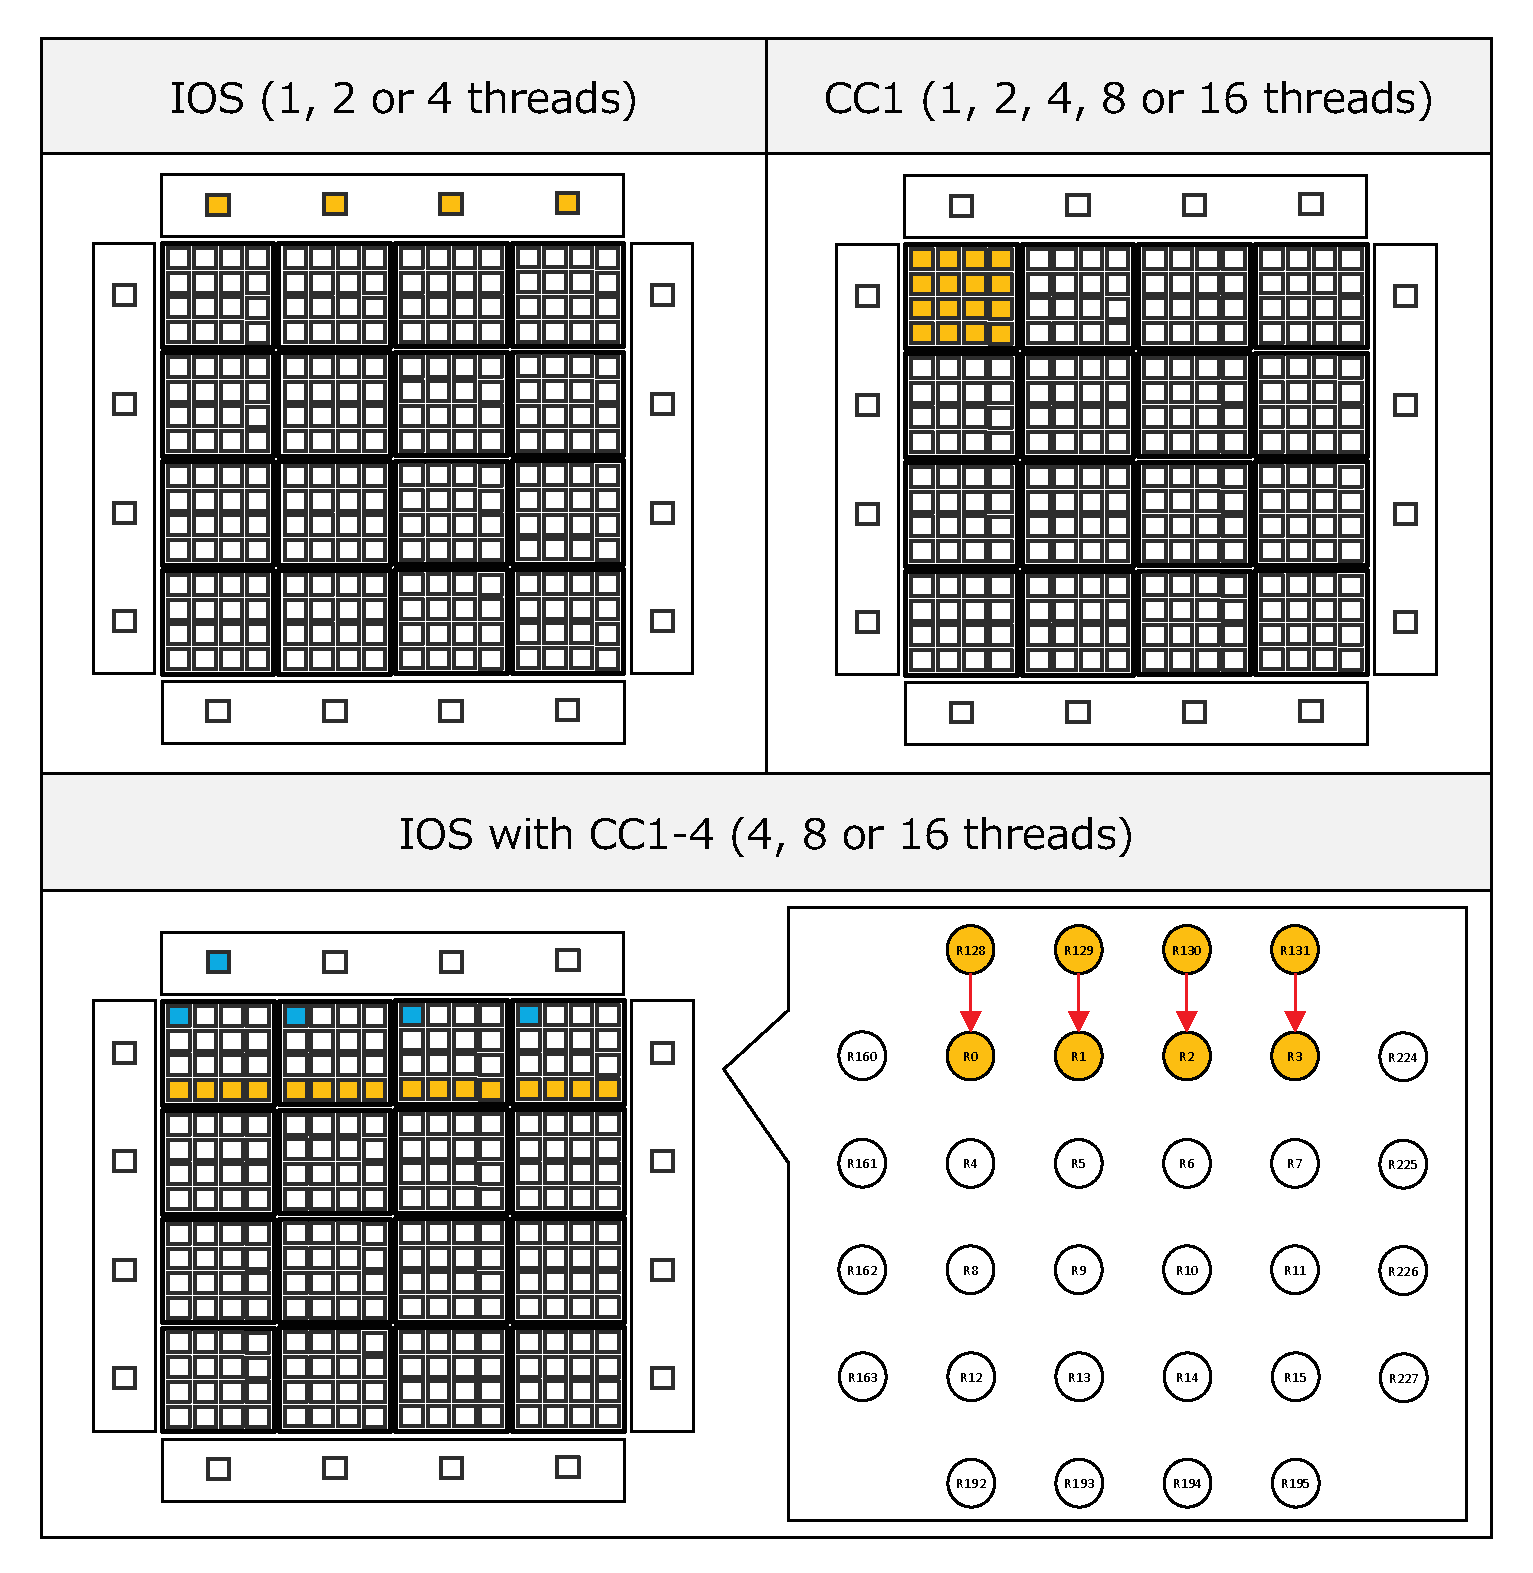
\includegraphics[width=0.8\linewidth]{../figure/matrix_calculation.eps}
  \caption{\label{fig:mat_calc}
    Matrix calculation situations.}
\end{figure}

\subsection{Influences of Cache and Memory Type}
\label{sec:cache_and_memory}
First, matrix calculation time with the cache in the IOS and CC is depicted in Fig. \ref{fig:mat_calc_cache}.
There are almost no differences between the IO DDR, IO SMEM, and CC SMEM due to the cache.
A 128 KB data cache in the IOS works well and compensates for the DDR delay.
Additionally, it is observed that calculation time scales exhibit a linear relation with the number of threads.
This corresponds to ideal behavior with respect to parallelization.

Second, matrix calculation time without a cache in the IOS and CC is shown in Fig. \ref{fig:mat_calc_uncache}.
The absence of a cache, results in a fourfold increase in the DDR and a large difference arises with respect to the SMEM.
Another notable result is that calculation speed in the CC SMEM exceeds that of the IO SMEM.
This characteristic is hidden in the calculation with the cache.
The computing cores physically involve the same cores in the IOS and CC, and thus it is considered that the characteristics and physical arrangement of the SMEM exert a significant effect.
This is an interesting result since there is a large difference that cannot be ignored.
It is also observed that calculation time exhibits a linear relation with the number of threads.
Furthermore, in the CC SMEM, the calculation speed without the cache exceeds that with cache.
This result is contrary to intuition, and a cache line problem is conceivable.
When a small data cache (8 KB) in a PE of the CC does not function adequately and an application always misses the cache, memory access will pay the time for a noncached data access and the cost to refill the cache line.
As a result, the memory access speed without the cache exceeds that with it.

% \begin{figure}[htbp]
%   \tabcolsep = 0.5mm              % side-margin in column
%   \begin{tabular}{cc}
%     \begin{minipage}[htbp]{0.49\textwidth}
%     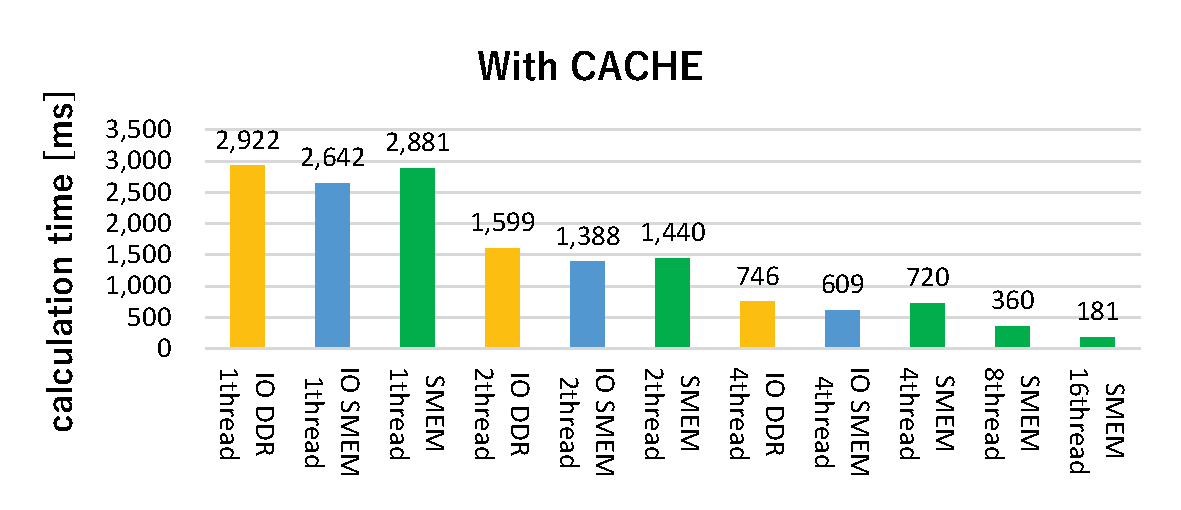
\includegraphics[width=1.0\linewidth]{../figure/BarGraph_matrix_with_cache.eps}
%       \caption{Matrix calculations in IOS and CC with cache.}
%       \label{fig:mat_calc_cache}
%     \end{minipage}   
%     &
%     % \setcounter{figure}{11}
%     \begin{minipage}[htbp]{0.49\textwidth}
%       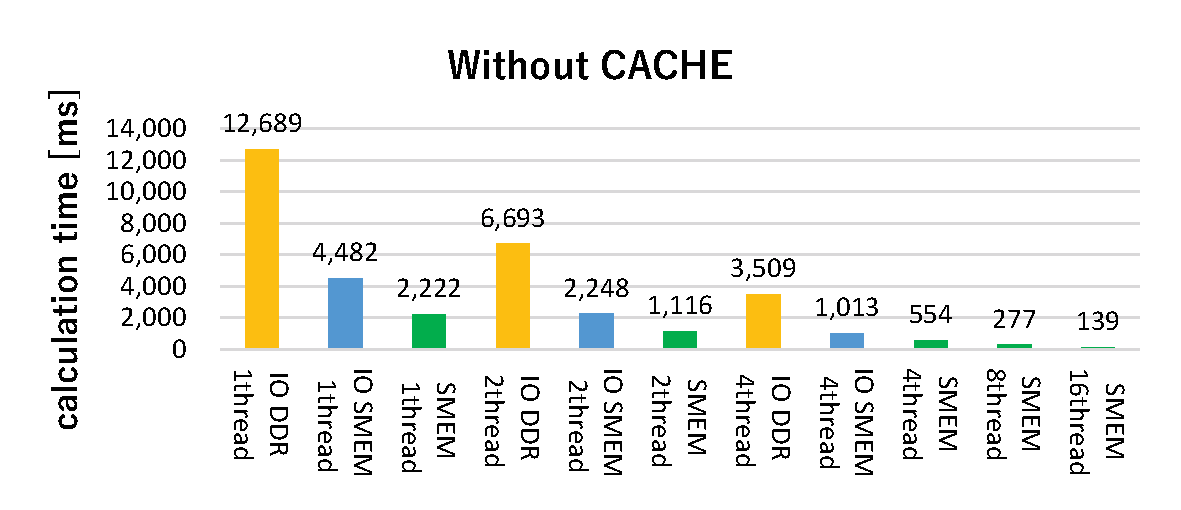
\includegraphics[width=1.0\linewidth]{../figure/BarGraph_matrix_without_cache.eps}
%       \caption{Matrix calculations in IOS and CC without cache.}
%       \label{fig:mat_calc_uncache}
%     \end{minipage}
%   \end{tabular}
% \end{figure}

\begin{figure}[htbp]
  \centering
  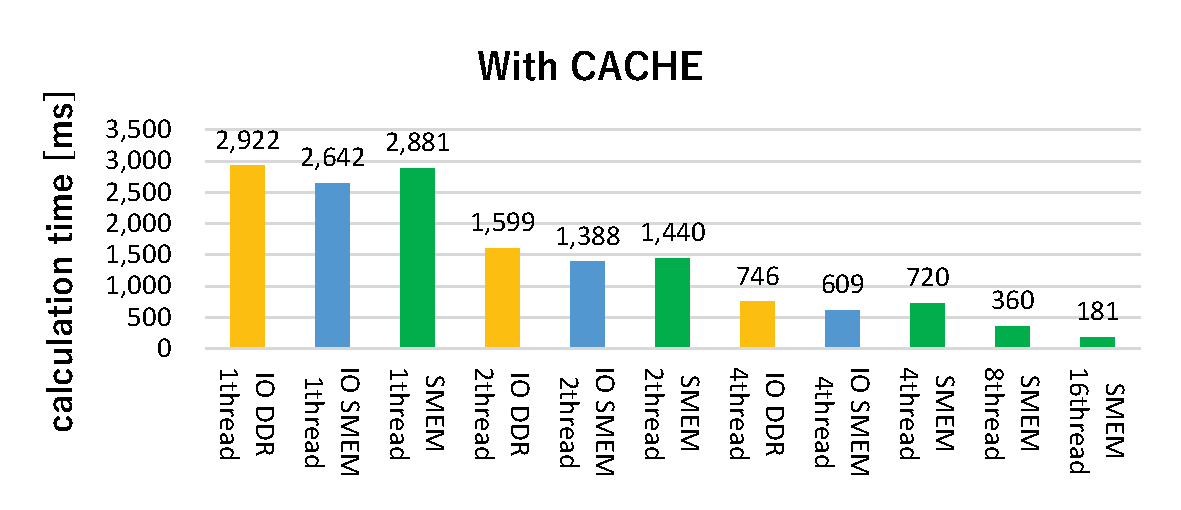
\includegraphics[width=1.0\linewidth]{../figure/BarGraph_matrix_with_cache.eps}
  \caption{Matrix calculations in IOS and CC with cache.}
  \label{fig:mat_calc_cache}
\end{figure}

\begin{figure}[htbp]
  \centering
  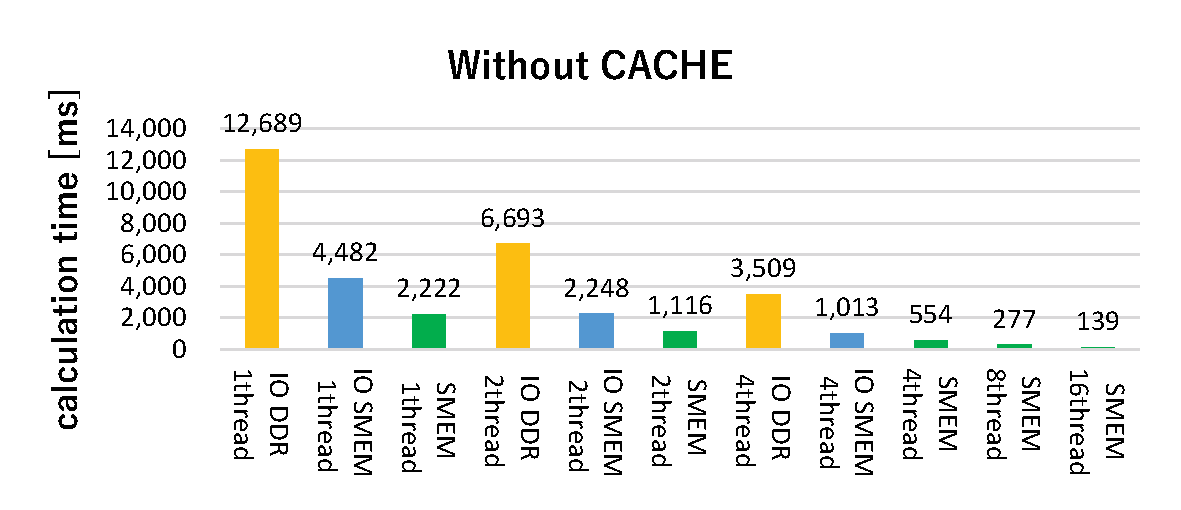
\includegraphics[width=1.0\linewidth]{../figure/BarGraph_matrix_without_cache.eps}
  \caption{Matrix calculations in IOS and CC without cache.}
  \label{fig:mat_calc_uncache}
\end{figure}

\subsection{Four CCs' Parallelization}
\label{sec:four_CCs}
Finally, matrix calculation with offload-computing in an IOS and CCs is shown in Figs. \ref{fig:mat_calc_offload_314} and \ref{fig:mat_calc_offload_640}.
In this case, it is assumed with respect to the calculation of large matrices that the total capacity exceeds 1 MB.
The offloading result is compared with the IO DDR (cached) owing to the aforementioned assumption.
The aggregate calculation is obtained by offloading on the four CCs to perform a multiplication of a tile of Mat A and a tile of the transpose of Mat B.
This produces an overhead irrespective of the number of threads as shown in Figs. \ref{fig:mat_calc_offload_314} and \ref{fig:mat_calc_offload_640}.

However, the speed involved in offloading the result exceeds that of the IO DDR (cached).
The result indicates several important facts.
First, D-NoC data transfer produces little overhead latency.
Second, the speed of DMA memory access to DDR exceeds that of the IO core's memory access, even if target memory is allocated on the DDR.
In the offloading case, a DMA accesses matrix buffers on the DDR and transfers the buffers from the IO DDR to each CC SMEM.
Subsequently, PEs in the CC access matrix buffer the calculation without a cache.
The overhead of data transfer and DMA memory access is small, and thus parallel data transmission and distributed memory are practical in the case of MPPA-256.
The impact of offloading increases when the matrix is large as shown in Fig. \ref{fig:mat_calc_offload_640}.
Only a portion of the matrix is allocated in CCs, and thus it is possible to handle larger matrix buffers.

Additionally, 640 KB matrices are prepared, and matrix calculation are evaluated with offload-computing.
The speed of the offloading result exceeds that of the IO DDR result with respect to the 314 KB matrices in Fig. \ref{fig:mat_calc_offload_314}.
In these offloading evaluations, each CC concurrently transmits calculation results to the IOS.
\comment{1-22}
When Matrix C in which calculation results are stored is allocated in the DDR, the NoC router's FIFOs sometimes overflow and cause an error due to memory access delay of the DDR.
The transmission protocol would ideally be expected to prevent this error, and flow control is intended as future work for MPPA-256.
Currently, to avoid this error, Matrix C must be allocated in the IO SMEM.
Note that the above evaluation results when Matrix C is allocated in the DDR.


\begin{figure}[htbp]
  \tabcolsep = 0.5mm              % side-margin in column
  \begin{tabular}{cc}
    \begin{minipage}[htbp]{0.49\textwidth}
      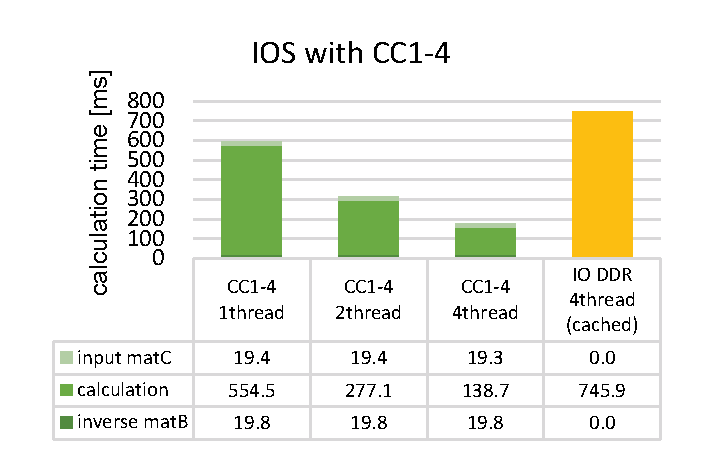
\includegraphics[width=0.9\linewidth]{../figure/BarGraph_matrix_with_CCs_314.eps}
      \caption{Matrix calculations with offload computing (314 KB matrix x 3).}
      \label{fig:mat_calc_offload_314}
    \end{minipage}   
    &
    % \setcounter{figure}{11}
    \begin{minipage}[htbp]{0.49\textwidth}
      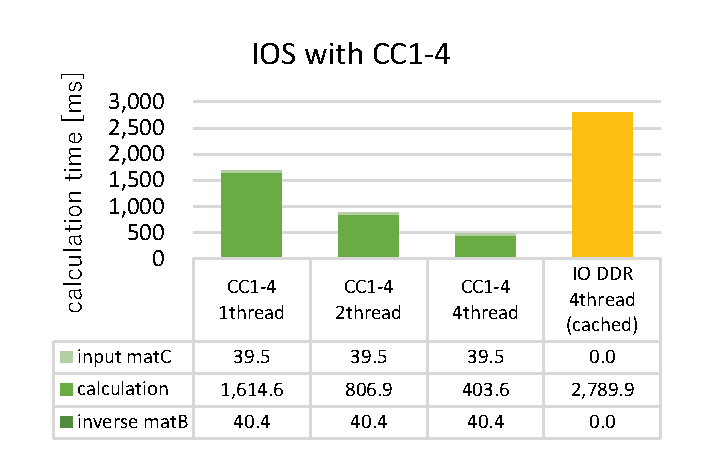
\includegraphics[width=0.9\linewidth]{../figure/BarGraph_matrix_with_CCs_640.eps}
      \caption{Matrix calculations with offload computing (640 KB matrix x 3).}
      \label{fig:mat_calc_offload_640}
    \end{minipage}
  \end{tabular}
\end{figure}

\section{Practical Application}
\label{sec:practical_application}
This work adopts a portion of a self-driving system and this section demonstrates the parallelization potential of the MPPA-256.
We selected an algorithm for vehicle self-localization written in C++ in Autoware, open-source software for urban self-driving \cite{autoware}, and a parallelized part of it.
The self-localization adopts the normal-distribution transform matching algorithm \cite{magnusson2009three} implemented in the Point Cloud Library \cite{pcl}.
A diagram depicting self-localization is shown in Fig. \ref{fig:ndt_matching_situation}.

% The self-localization algorithm is primarily divided into two processes: \emph{RadiusSearch} which searches for several nearest neighbor points for each query and calculates the distance, and \emph{Derivatives} which calculates the derivative to determine the convergence of the matching operation.
% As shown in Fig. \ref{fig:ndt_matching_situation}, 
% This evaluation parallelized \emph{Derivatives} onto 16 CCs and the remainder of the algorithm was executed on the IOS with its four cores.
% To parallelize \emph{RadiusSearch}, the algorithm of the nearest neighbor search needs to be redesigned because the data to be searched exceeds 1 MB.
% Redesigning this algorithm will be part of a future work.

The self-localization algorithm is composed primarily of the \emph{computeTransform} function which searches for several nearest neighbor points for each scan query and calculates a matching transformation.
This evaluation parallelized a part of \emph{computeTransform} onto 16 CCs and the remainder of the algorithm was executed in parallel on the IOS with its four cores.
To parallelize the remainder of \emph{computeTransform} in CCs, the algorithm of the nearest neighbor search must be redesigned because the data to be searched exceeds 1 MB.
Redesigning this algorithm is reserved for future work, and there is room for improvement through the parallelization potential of the MPPA-256.

As shown in Fig. \ref{fig:ndt_matching}, the evaluation of the parallelized self-localization algorithm indicates the average execution time for each convergence and demonstrates that the parallelization accelerates the \emph{computeTransform} process.
% Because the reduction of the execution time of \emph{computeTransform} involves reducing the number of loops for convergence, the execution times of \emph{RadiusSearch} and other parts are also shortened.
The query can be assumed to be 10 Hz in many automated driving systems.
Thus, this tuning successfully meets the deadline.
This parallelized algorithm was executed on simulated and real car experiments in our test course and worked successfully.
The steering, accelerator, and brake are automatically controlled based on the results of MPPA-256.
A demonstration video of the adaptation of the parallelized self-localization algorithm to Autoware on eMCOS can be seen at: https://youtu.be/wZyqF90c5b8  

\begin{figure}[htbp]
  \tabcolsep = 0.5mm              % side-margin in column
  \begin{tabular}{cc}
    \begin{minipage}[htbp]{0.49\textwidth}
      \centering
      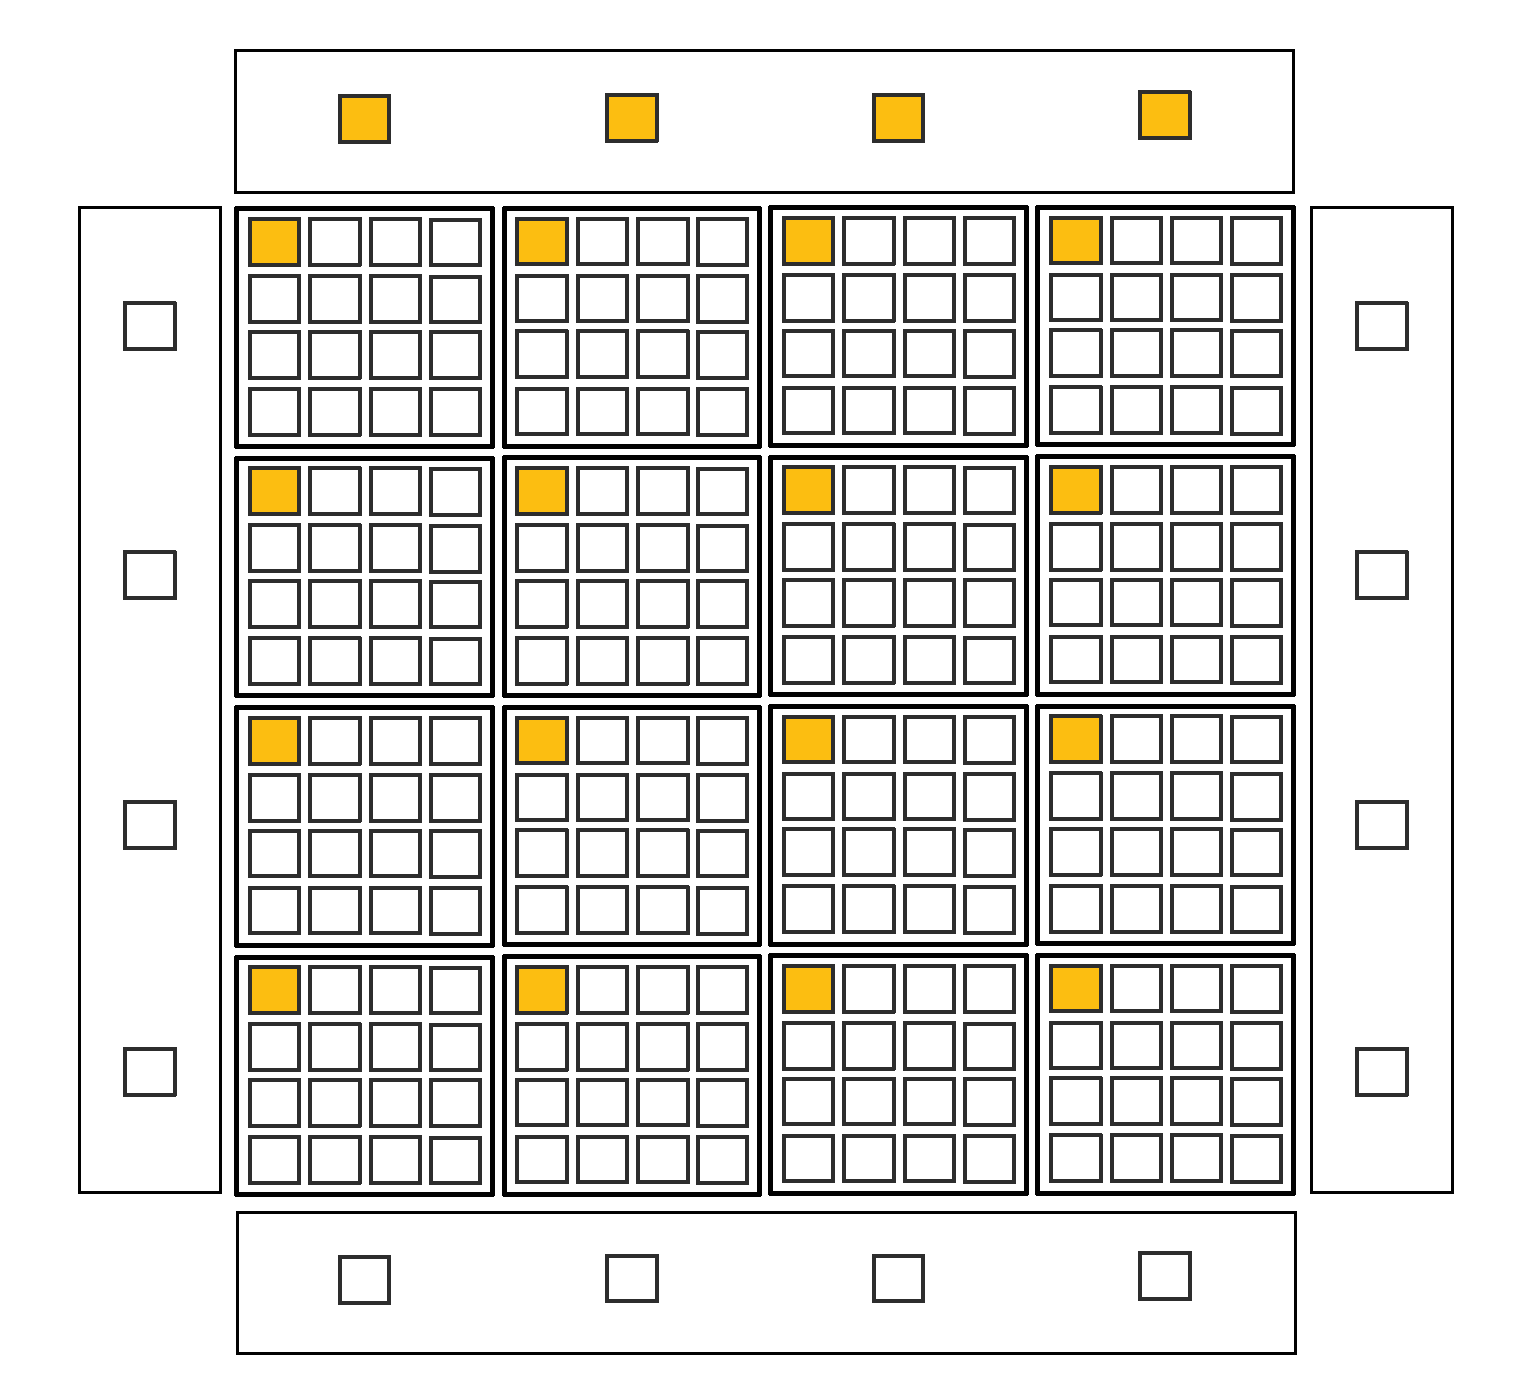
\includegraphics[width=1.0\linewidth]{../figure/ndt_matching.eps}
      \caption{\label{fig:ndt_matching_situation}
      A situation of vehicle self-localization execution.}
    \end{minipage}   
    &
    % \setcounter{figure}{11}
    \begin{minipage}[htbp]{0.49\textwidth}
      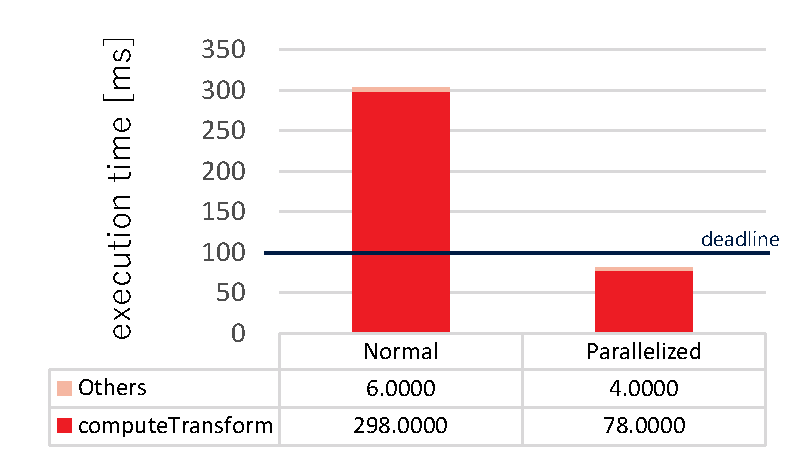
\includegraphics[width=1.0\linewidth]{../figure/BarGraph_ndt_matching.eps}
      \caption{\label{fig:ndt_matching}
      Vehicle self-localization of the partially parallelized self-driving application.}
    \end{minipage}
  \end{tabular}
\end{figure}

% \begin{figure}[htbp]
%   \centering
%   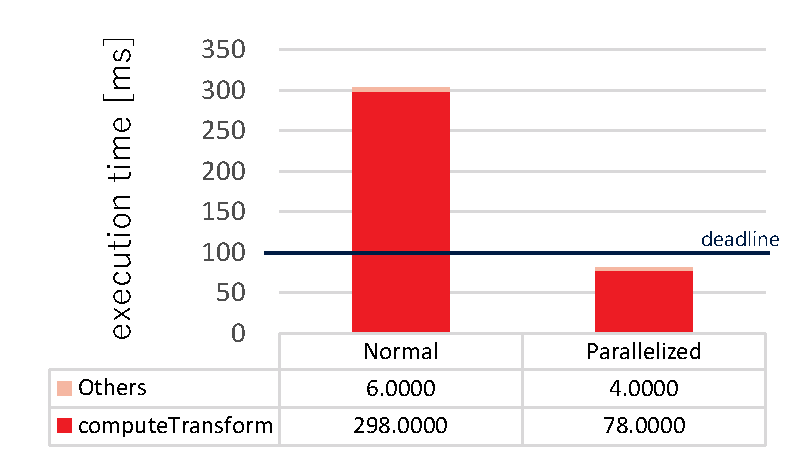
\includegraphics[width=0.8\linewidth]{../figure/BarGraph_ndt_matching.eps}
%       \caption{\label{fig:ndt_matching}
%   Vehicle self-localization of the partially parallelized self-driving application.}
%     \end{figure}

\section{Lessons Learned}
\label{sec:lessons}
\comment{TBD: 3-4}
Thus far, in Section \ref{sec:evaluations}, we have quantitatively clarified the characteristic of data transfer and parallel computing on NoC-based embedded many-core platforms.
We can obtaine insight and guidelines for users and developers of NoC-based embedded many-core platforms through MPPA-256.

From evaluations of D-NoC data transfer, we can learn two lessons: the influences of NoC routing and DMA.
First, data transfer latencies between clusters are hardly influenced by routing for users as shown in Figs. \ref{fig:DDR_tx}, \ref{fig:DDR_uc}, \ref{fig:IO_SMEM_tx}, and \ref{fig:IO_SMEM_uc}.
Software transactions of transmitting and receiving in routers and RM are dominant factors for latencies.
This is understandable owing to the minimized traffic conflicts of the evaluation setting.
However, when the influence of routing comes to intensive concurrent traffic over a large portion of the network, different routes might still have nontrivial impacts on the end-to-end data transfer delay, especially for a detour route of a longer length.
Second, in the IOS, the latency of a UC is not significantly affected by the memory location, the DDR or SMEM, at which the transferred buffer is allocated from the evaluation of Fig. \ref{fig:tx_uc_log}.
The merit of the UC is profitable for users because this is a common situation for transferrinng data from the DDR to the CC SMEM using the UC, especially for large amount of data.

From microbenchmarks of matrix calculation, we can learn three lessons of memory access: characteristics of the SMEM, influences of a cache, and data flow control on D-NoC.
First, the memory access speed of the CC SMEM exceeds that of the IO SMEM as shown in Fig. \ref{fig:mat_calc_uncache}.
There is a significant difference, which is a major reason to work actively in the CC.
Second, we indicate quantitatively that the calculation speed without the cache in the CC SMEM in Fig. \ref{fig:mat_calc_uncache} exceeds that with the cache in Fig. \ref{fig:mat_calc_cache}.
It is generally known that there is cache overhead when a miss hit occurs frequently, but it is notable that there is a substantial difference that cannot be ignored by the influences of a cache line.
Third, when data are transferred in parallel from multiple CCs to the IO DDR, NoC routers' FIFO sometimes overflows owing to memory access delays of the DDR.
This would ideally be expected to prevented by the transmission protocol and flow control.

From the practical application viewpoint, since we parallelize the vehicle self-localization algorithm of the self-driving system, NoC-based embedded many-core systems can be used practically in real environments.
We applied parallel data transfer from an IOS to CCs and parallel computing on the IOS and CCs by using the CC SMEM as scratch pad memory.    
We also conducted demonstration experiments with real environments and confirmed the practicality of NoC-based embedded many-core systems.

\chapter{Related Work}
\label{sec:related_work}
This section compares many-core platforms and discusses previous work related to multi-/many-core platforms.
First, comparison of many-core platforms to other platforms is discussed.
Second, the Kalray MPPA-256 which this work focuses on is compared to other COTS multi-/many-core components, and we summarize the features of MPPA-256.
Finally, discussions of previous work and comparisons with them are described.

% Recently, studies indicate that the single core processors are characterized by limited computation performance.
% Pollack stated that a single core is inefficient \cite{pollack1999new} and that Moore's law \cite{moore2006cramming} is no longer applicable.
% Therefore, extant CPUs are not sufficient to satisfy increasing computation demands.
% The shift from a single core in real-Time and embedded systems has occurred \cite{saidi2015shift}. 
% Many other platforms including many-core are developed and researched by current studies.

Table \ref{tb:comparison_platforms} summarizes the features of many-core platforms with those of other platforms.
For instance, the GPU is a powerful device to enhance computing performance and has great potential in specific areas (for e.g., image processing, and learning).
\comment{1-24}
However, th GPU is mainly used for a specific purpose and its predictability is not suitable for real-time systems.
It is difficult to use a GPU for many kinds of applications and to guarantee its reliability due to the GPU architecture.
Many-core processors based on CPU are significantly superior to GPU with respect to software programmability and timing predictability.
\comment{1-25}
Additionally, it is commonly known that many-core platforms such as MPPA-256 involve a reasonable power consumption \cite{kanter2015kalray}.
In contrast, the GPU consumes a significant amount of power and generates considerable heat.
This is a critical problem for embedded systems.
FPGAs are also high-performance devices when compared to CPUs.
They are efficient in terms of power consumption.
FPGAs guarantee predictability and efficient processing.
% They are suitable for time-critical computing \cite{de2015kalray}.
\comment{1-26}
% However, DSPs cannot be used for many kinds of applications and programming.
However, FPGAs are difficult for software developers and are not a substitute for CPU since their software model is significantly different from that of CPU.
Many-core platforms can potentially replace single/multi core CPU as they possess ease of programming and scalability.

Based on the aforementioned background, many COTS multi-/many-core components are developed and released by several vendors.
(e.g., MPPA-256 by Kalray, \cite{de2014time}, Tile-Gx by Tilera \cite{ramey2011tile}, \cite{schooler2010tile}, Tile64 by Tilera \cite{bell2008tile64}, and Xeon Phi by Intel \cite{chrysos2014intel}, \cite{chrysos2012intel}, Single-chip Cloud Computer (SCC) by Intel \cite{baron2010single}).
The present work focuses on the Kalray MPPA-256, which is designed for embedded applications.
Kalray \cite{de2014time} presented clustered many-core architectures on the NoC that pack 256 general-purpose cores with high energy efficiency.


\comment{1-27}
MPPA-256 is superior to other COTS multi-/many-core components in terms of the scalability of the number of cores and the power efficiency, as shown in Table \ref{tb:comparison_manycore}.
\comment{1-28}
In terms of scalability, MPPA-256 uses 256 cores, whereas other COTS multi-/many-core components have 64 cores or the number of cores around it.
This scalability of cores is attributed to the NUMA memory architecture; each cluster of 16 cores contains its own local shared memory.
The precise hardware model is described in Section \ref{sec:hardware_model}.
When all cores share the global DDR memory as in other platforms excluding MPPA-256, specific bus/network routes receive extremely large loads and memory access contention frequently occurs.
Local shared memory reduces the above problems and helps the scalability of the number of cores.
% This is why MPPA-256 has succeeded in scaling up to 256 cores and what the ``scalability'' column of Table \ref{tb:comparison_manycore} means.
However, the NUMA memory architecture restricts the capacity of the memory and requires a data copy from the DDR with NoC.
This restriction makes the use of existing applications difficult especially in the case of applications that require more memory.
As a result, owing to the NUMA memory architecture, the portability of code porting to MPPA-256 is inferior to that of other COTS platforms, as shown in Table \ref{tb:comparison_manycore}.

In terms of power efficiency, MPPA-256 realizes superior energy efficiency despite its large number of cores \cite{kanter2015kalray}.
The total clock frequency per watt is the highest of the current COTS multi-/many-core components.
The power consumption of the MPPA processor ranges between 16 W at 600 MHz and 24 W at 800 MHz.
% While MPPA-256 and TILE64 \cite{bell2008tile64} target the embedded systems, other COTS components consider the HPC accelerator.
% Their clock frequency per core exceeds that of embedded solutions.
We must distinguish the COTS multi-/many-core components according to their requirements with reference to Table \ref{tb:comparison_manycore}.
MPPA-256 is typically accepted with respect to many-core platforms and the model has been used in previous work \cite{becker2016contention}, \cite{carle2014static}, \cite{perret2016mapping}, \cite{perret2016predictable}.

Previous work has examined real-time applications on many-core platforms, including MPPA-256.
Multiple opportunities and challenges of multi-/many-core platforms are discussed in \cite{saidi2015shift}.
The shift to multi-/many-core platforms in real-time and embedded systems is also described. 

Based on the above background, several task mapping algorithms for multi/many-core systems have been proposed \cite{carle2014static}, \cite{faragardi2014communication}, \cite{perret2016mapping}.
Airbus \cite{perret2016mapping} proposes a method of directed acyclic graph (DAG) scheduling for hard real-time applications using MPPA-256.
In \cite{faragardi2014communication}, a mapping framework is proposed on the basis of AUTOSAR which is applied as a standard architecture to develop automotive embedded software systems \cite{furst2009autosar}.
AUTOSAR task scheduling considering contention in shared resources is presented in \cite{becker2016contention}.

By examining the above mapping algorithms of real-time applications, previous work \cite{deDinechin2014GSN}, \cite{denet2017work}, \cite{kanter2015kalray}, \cite{perret2016predictable} has analyzed the potential of MPPA-256 and data transfer with NoC, as shown in Table \ref{tb:comparison_relatedwork}.
MPPA-256 is introduced and its performance and energy consumption are reported in \cite{kanter2015kalray}.
However, this report contains few evaluations and does not refer to data transfer with NoC and memory access characteristics.
Data transfer with NoC in MPPA-256 is described, and NoC guaranteed services are analyzed in \cite{deDinechin2014GSN} and \cite{denet2017work}.
While the theoretical analysis is thorough in these works, the practical evaluations are poor and parallel data transfer is not referred to.
The authors of Ref. \cite{perret2016predictable} focused on the predictable composition of memory access.
An analysis of their work identified the external DDR and the NoC as the principal bottlenecks for both the average performance and the predictability on platforms such as MPPA-256.
Although the analysis examined the memory access characteristics of the external DDR and provided notable lessons, a solution for the DDR bottleneck was not examined and practical evaluations were lacking.

\begin{landscape}
  % \renewcommand{\arraystretch}{1.2}
  \begin{table*}[t]
    \caption{\label{tb:comparison_platforms}
      Comparison of Many-core Platform to CPU, GPU, and FPGA}
    \centering
    % \scriptsize	                    % text size
    % \tabcolsep = 0.4mm              % side-margin in column
    \begin{tabular}{c|cccccccccc}
      \hline
      & \multirow{2}{*}{performance} & \multirow{2}{*}{power/heat} & \multirow{2}{*}{real-time} & software & \multirow{2}{*}{costs} & multiple\\
      &&&&& development && instruction \\
      \hline
      \hline
      CPU & & L & \(\checkmark\) & \(\checkmark\) & \(\checkmark\) & L \\
      GPU & \(\checkmark\) &  &  & L & \(\checkmark\)\\
      % DSP & L & L & \(\checkmark\) & \(\checkmark\) & L & \(\checkmark\) & \\
      FPGA & \(\checkmark\) & L & L &  & L & \\
      Many-core Platform & \(\checkmark\) & \(\checkmark\) & \(\checkmark\) & \(\checkmark\) & L & \(\checkmark\) \\
      \hline
    \end{tabular}
    \begin{flushright}
        \comment{1-23} \textasteriskcentered In a table, ``L'' means ``limited''.
    \end{flushright}
  \end{table*}

  % \renewcommand{\arraystretch}{1.2}
  \begin{table*}[t]
    \caption{\label{tb:comparison_manycore}
      Comparison of Many-core Platforms}
    \centering
    % \scriptsize	                    % text size
    % \tabcolsep = 1.5mm              % side-margin in column
    \begin{tabular}{c|cccc}
      \hline
      & \multirow{2}{*}{scalability} & power  & code & \\
      & & efficiency & transplant & \\
      \hline
      \hline
      Kalray MPPA-256 \cite{de2014time} & \(\checkmark\) & \(\checkmark\) & L & \\
      Tilera Tile series \cite{bell2008tile64} &  & L & \(\checkmark\) & \\
      Intel Xeon Phi \cite{chrysos2014intel} \cite{chrysos2012intel} &  &  & \(\checkmark\) & \\
      Intel SCC \cite{baron2010single} &  &  & \(\checkmark\) & \\
      \hline
    \end{tabular}
  \end{table*}  
  % \renewcommand{\arraystretch}{1.2}
  \begin{table*}[t]
    \caption{\label{tb:comparison_relatedwork}
      Comparison of Previous Work}
    \centering
    \scriptsize	                    % text size
    % \tabcolsep = 2mm              % side-margin in column
    \begin{tabular}{c|ccccccccc}
      \hline
      & performance & data transfer & memory access & \multirow{2}{*}{real applications} & parallel data & \\
      & analysis & analysis with NoC & characteristics & & transfer & \\
      \hline
      \hline
      Kalray clusters calculate quickly \cite{kanter2015kalray} & L &  &  &  &  & \\
      Network-on-Chip Service Guarantees \cite{denet2017work} &  & \(\checkmark\) &  &  &  & \\
      Predictable composition of memory accesses \cite{perret2016predictable} &  & \(\checkmark\) & \(\checkmark\) &  &  & \\
      this paper & \(\checkmark\) & \(\checkmark\) & \(\checkmark\) & \(\checkmark\) & \(\checkmark\) & \\
      \hline
    \end{tabular}
  \end{table*}
\end{landscape}


\chapter{Conclusions}
\label{sec:conclusion}
% This paper has conducted quantitative evaluations that examined end-to-end latencies with embedded many-cores based on NoC, the scalability of parallelization, and the characteristics of the memory access speed.
% From various experiments, we have evaluated the capabilities of the currently available data transfer methods and the parallelization potential for many-core computing based on NoC.
% Our experimental results will allow system designers to choose appropriate system designs based on the requirements of their latency-sensitive many-core applications beyond an intuitive expectation.
In this work, we conducted quantitative evaluations of data transfer methods on NoC technology, microbenchmarks with matrix calculation, and a practical application with NUMA many-core platforms such as MPPA-256.
Evaluations indicate latency characteristics on NoC platforms, influences of data allocation, and the scalability of parallelization.
Our experimental results will allow system designers to select appropriate system designs.
Last, parallelization of a real application proved the practicality of NoC-based embedded NUMA many-core platforms.

In future work, we will use benchmark applications such as that in \cite{che2010characterization} for further analysis.
In addition, considering above the results, we will port real-time systems such as that in \cite{maruyama2016ros2} on CCs, and we propose the parallelization of memory intensive algorithms, such as the nearest neighbor search in Section \ref{sec:practical_application}.


%%%%%%%%%%%%%%%%%%%%%%%%%%%%%%%%%%%%%%%%%%%%%%%  テンプレート非依存部(終了)  %%%%%%%%%%%%%%%%%%%%%%%%%%%%%%%%%%%%%%%%%%%%%%%  


% use section* for acknowledgment
% \ifCLASSOPTIONcompsoc
  % The Computer Society usually uses the plural form
  % \chapter*{Acknowledgments}
% \else
  % regular IEEE prefers the singular form
%   \chapter*{Acknowledgment}
% % \fi
%   This paper was partly supported by Toyota Motor Company, eSOL, and Kalray.
%   In addition, this research was partially supported by JST, PRESTO.

% \ifCLASSOPTIONcaptionsoff
  % \newpage
% \fi

% \renewcommand{\baselinestretch}{0.8}

% \comment{2-5}
% \comment{TBD: 3-6}
% \bibliographystyle{IEEEtran}
% \bibliography{./reference.bib}

% \end{document}



%%%%%%%%%%%% Apendix %%%%%%%%%%%%%%%%%%%%%%%%%%%%%%%%%%%%%%%
\appendix

\setcounter{chapter}{1}
\setcounter{section}{0}
\setcounter{figure}{0}

\chapter*{Appendix A: Robot Operating System (ROS)}
\addcontentsline{toc}{chapter}{Appendix A: Robot Operating System (ROS)}

As mentioned earlier, Autoware is based on ROS \cite{quigley2009ros},
\cite{rosorg}, which is a component-based middleware framework developed
for robot applications. 
ROS is designed to enhance modularity of robot applications at a
fine-grained scale and is made suitable for distributed systems, while
respecting efficient development.
Since autonomous vehicles require many software packages, ROS is a
strong basis to develop Autoware.

In ROS, the system is abstracted by \emph{nodes} and \emph{topics}.
The \emph{nodes} represent individual component modules, whereas the \emph{topics} hold input and output data between \emph{nodes} as shown in Figure \ref{fig:ros_pubsub}.
ROS \emph{nodes} are usually standard C++ programs.
They can use any other software libraries installed in the system.

Communication among \emph{nodes} is based on a publish/subscribe model.
This is a strong abstraction model for compositional development.
In this model, \emph{nodes} communicate by passing \emph{messages} via a \emph{topic}. 
A \emph{message} has a simple data structure (much like C structs) defined by .msg files.
\emph{Nodes} identify the content of the \emph{message} by the \emph{topic} name.
As a \emph{node} publishes a \emph{message} to a \emph{topic}, another \emph{node} subscribes to the \emph{topic} and utilizes the \emph{message}. 
For example, in Figure \ref{fig:ros_pubsub}, the ``Camera Driver'' \emph{node} sends \emph{messages} to the ``Images'' \emph{topic}. 
The \emph{messages} in the \emph{topic} are received by the ``Traffic light Recognition'' \emph{node} and ``Pedestrian Detection'' \emph{node}.
\emph{Topic} is also managed by first-in, first-out queues when accessed by multiple \emph{nodes} simultaneously.
Meanwhile, ROS \emph{nodes} can launch several threads implicitly.
Real-time issues, however, must be addressed.

ROS also provides an integrated visualization tool, called RViz, and a
data-driven simulation tool, called ROSBAG. 
Figure \ref{fig:rviz_autoware} (a) shows examples of visualization for perception tasks in Autoware with RViz.
The RViz viewer is useful for checking the status of tasks.
The ROSBAG is a set of tools for recording from and playing back to ROS \emph{topics}.
It provides us development environments to test self-driving algorithms without hardware devices such as a vehicle and sensors devices.
This is also useful for efficient development.

\begin{figure*}[!htbp]
  \centering
  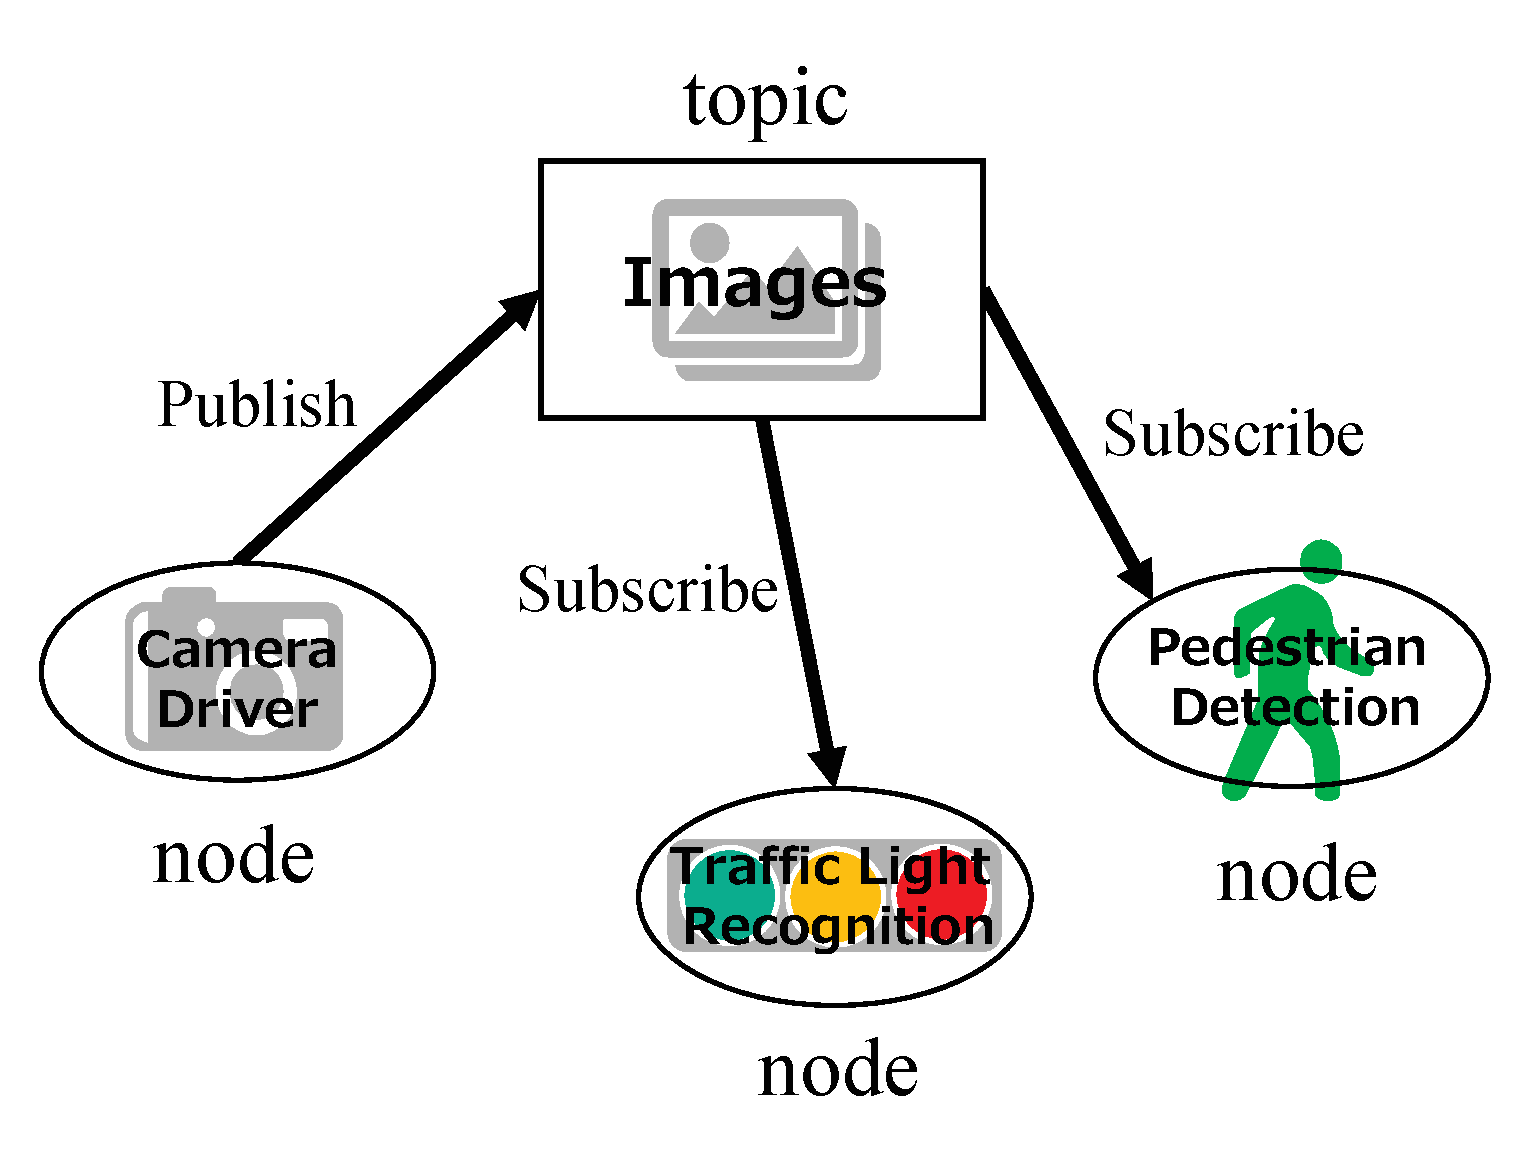
\includegraphics[width=0.8\linewidth]{../figure/ros_pubsub.eps}
  \caption{\label{fig:ros_pubsub}
 The publish/subscribe model in ROS.}
\end{figure*}



\setcounter{chapter}{2}
\setcounter{section}{0}
\setcounter{figure}{0}

\chapter*{Appendix B: Autoware}
\addcontentsline{toc}{chapter}{Appendix B: Autoware}

\section{System Model}
\label{sec:system_model}

\begin{figure}[!htbp]
  \centering
  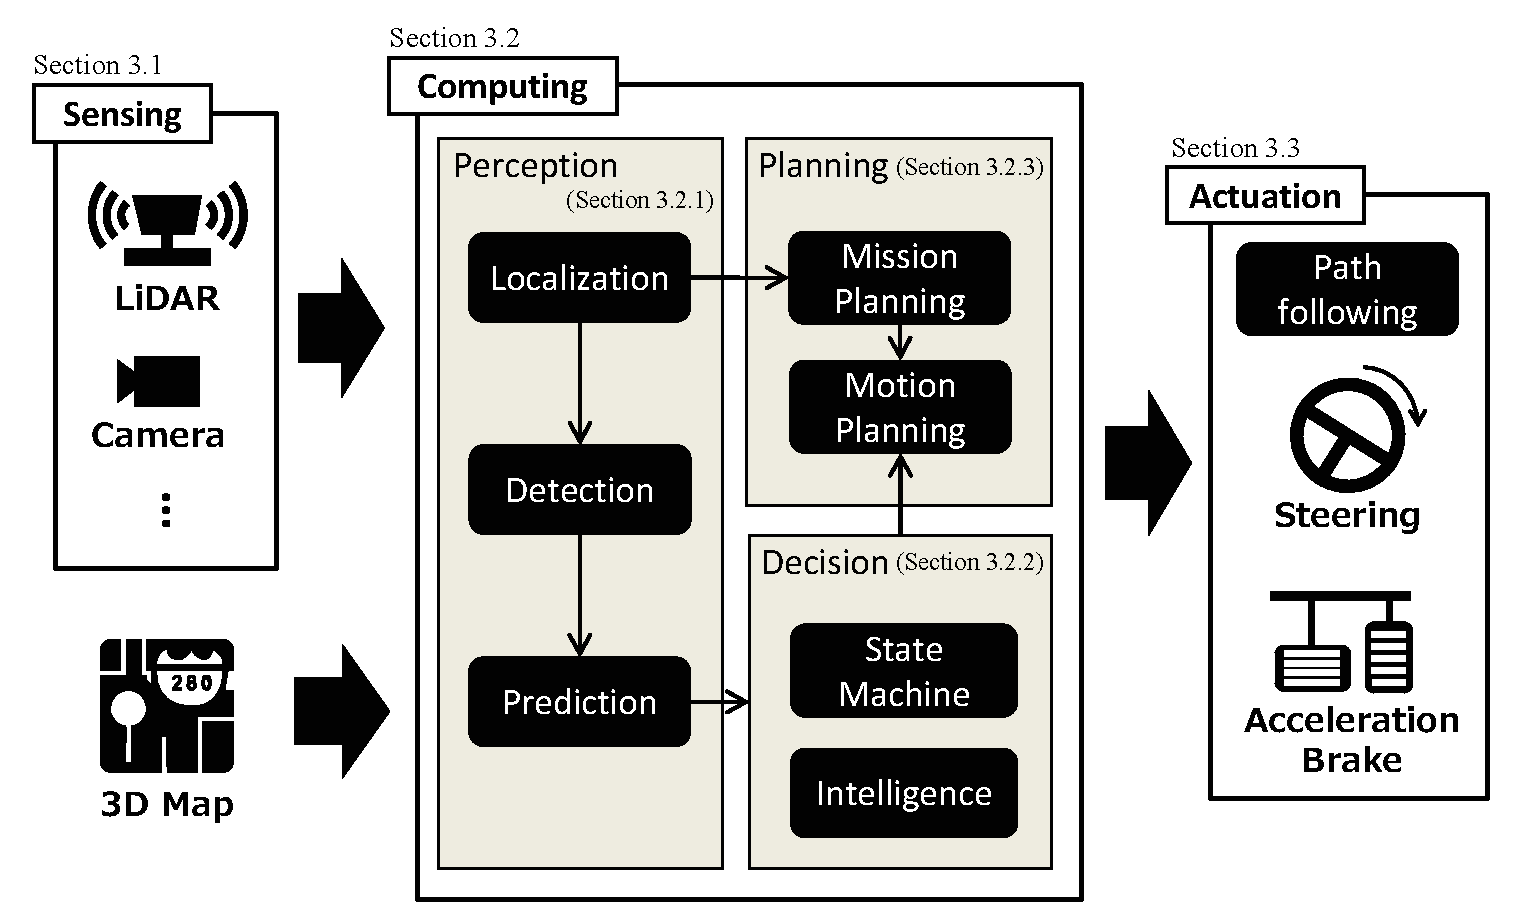
\includegraphics[width=0.6\linewidth]{../figure/system_model.eps}
  \caption{\label{fig:system_model}
    Basic control and data flow of autonomous vehicles.}
\end{figure}

Autonomous vehicles as cyber-physycal systems can be abstracted by
sensing, computing, and actuation, as shown in Figure
\ref{fig:system_model}.
Preferred sensing devices for urban-area self-driving, in particular,
include laser scanners (LiDAR) and cameras.
Actuation corresponds to manipulation of steering and stroking whose
twisted control commands are often generated by the path following module.
The computing intelligence is the major part of self-driving technology.
For instance, scene recognition requires localization, detection, and
prediction modules, while path planning falls into mission-based and
motion-based modules.
Each module employs corresponding algorithms.
Those implemented in Autoware, in particular, are introduced in Section
\ref{sec:autoware}.

Figure \ref{fig:system_model} shows a basic control and data flow of
autonomous vehicles.
Sensing devices acquire environmental information as input data for the
computing intelligence.
3D maps are also becoming more and more commonplace for self-driving
technology, especially for urban areas, to complement sensing and
computing capabilities of autonomous vehicles by high-definition and
high-resolution geographical information.
Leveraging these pieces of information, for example, the accuracy of
localization and detection can be improved highly without causing their
algorithms to become more complex.
Typical outputs of the computing intelligence are angular and linear
velocity values, which correspond to the commands for steering and
stroking, respectively.

\section{System Stack}

\begin{figure*}[!htbp]
  \centering
  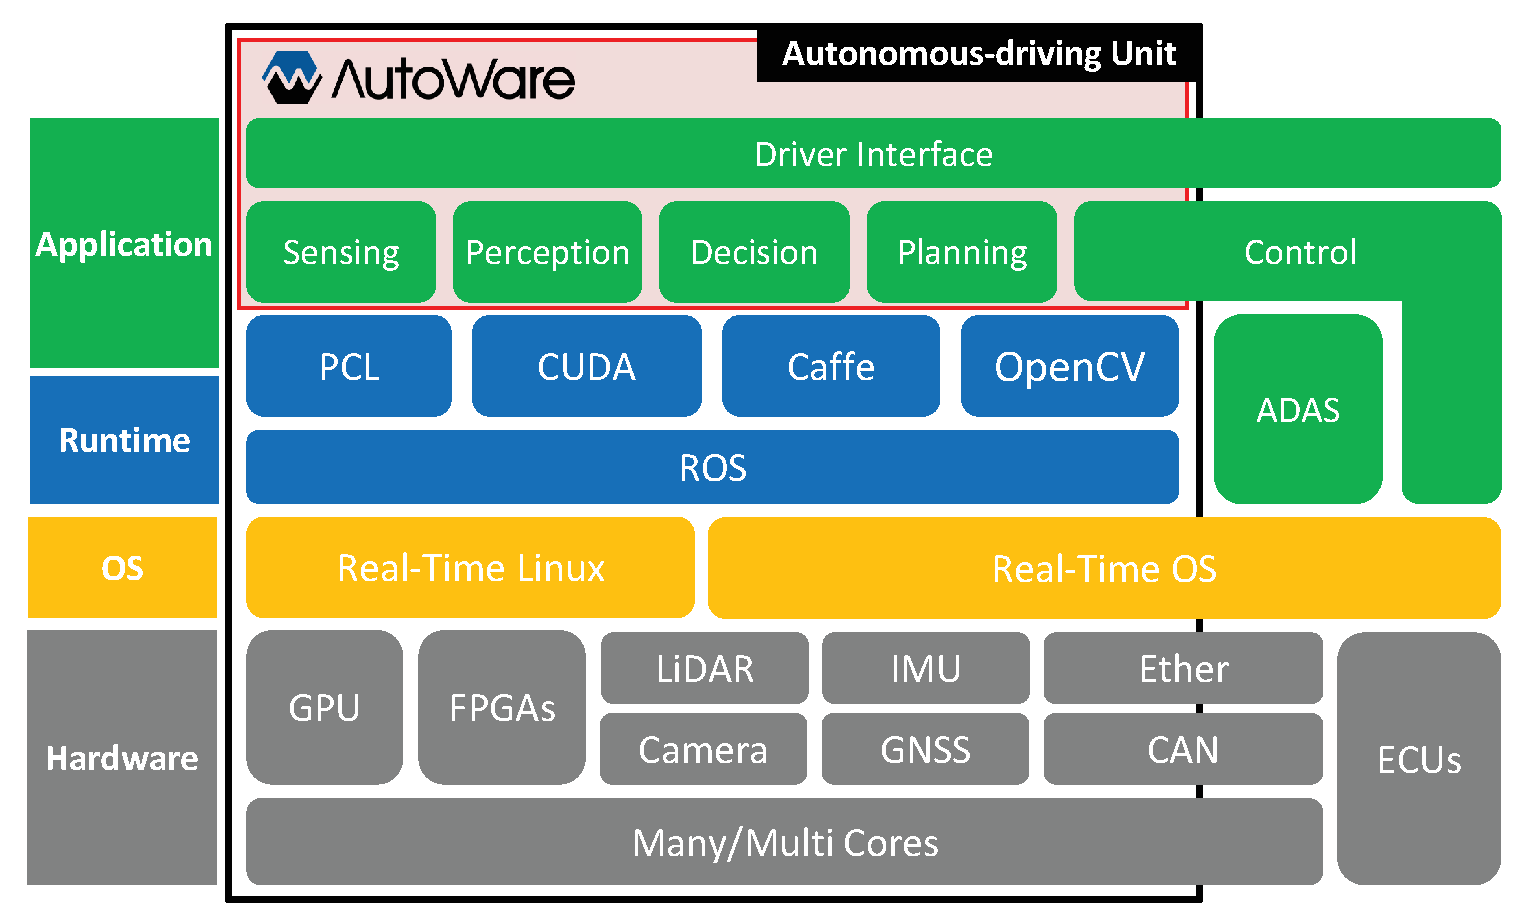
\includegraphics[width=0.6\linewidth]{../figure/system_stack.eps}
  \caption{\label{fig:system_stack}
  Complete system stack of autonomous vehicles using Autoware.}
\end{figure*}

We build the complete system stack of autonomous vehicles on top of
integrated platforms using open-source software, as shown in
Figure~\ref{fig:system_stack}.
The primary target of self-driving technology presented in this paper is
 set for urban areas rather than freeways and highways.
We develop Autoware which is a popular
open-source software project developed for urban-area autonomous
vehicles.
Autoware is based on Robot Operating System (ROS) and other
well-established open-source software libraries, as shown in
Figure~\ref{fig:system_stack}.
We introduce a brief overview of ROS separately in Section~\ref{sec:ros}.
Point Cloud Library (PCL) \cite{pcl} is mainly used to manage LiDAR
scans and 3D maps.
It is also used for data filtering and visualization.
CUDA \cite{cuda} is a programming framework for general-purpose
computing on GPUs (GPGPU).
Due to compute-intensive tasks in autonomous vehicles, GPUs and CUDA are
promising solutions for self-driving technology, though this paper does
not focus on them.
Caffe \cite{jia2014caffe}, \cite{caffe} is a native deep learning
framework made with expression, speed, and modularity in mind.
OpenCV \cite{opencv} is a popular computer vision library for image
processing.

Autoware provides a rich set of software packages, including sensing,
perception, decision making, planning, and control modules.
Many drive-by-wire vehicles can be transformed into autonomous vehicles
by installing Autoware.
In several countries, Autoware has already succeeded in demonstration of
autonomous vehicles driving for a long distance of public roads in urban
areas. 
Recently, automotive manufacturers and suppliers have also started
adopting Autoware as a baseline of their prototype autonomous vehicles.

In this section, we also briefly introduce hardware pieces of autonomous
vehicles assumed in this paper.
To apply our system stack, we need to make a modification to commercial
vehicles so that they can be controlled by external computers through
some secure gateway, and also install sensors on the vehicles.
The interface among the vehicles, computers, and sensors could be the
CAN bus, Ethernet, and/or USB 3.0.
The specification of sensors and computers, however, highly depends on
the functional requirement of each autonomous vehicle.
Autoware supports various sensing devices, but our prototype system
specifically uses Velodyne HDL-32e LiDAR scanners and PointGrey
Grasshopper3 cameras.
Autoware also supports various computers.
Many users often run Autoware on desktop and laptop computers.
In this paper, we specifically use NVIDIA DRIVE PX2, though our previous
work partly ported Autoware to another embedded computing platform,
called Kalray Massively Parallel Processor Array
(MPPA)~\cite{yuya2017exploring}. 

\section{Algorithms}
\label{sec:system_model}

In this section, we present the detail of Autoware in accordance with
Figure~\ref{fig:system_model}, with a particular emphasis on the modules
that we develop and extend for DRIVE PX2.
The remaining pieces of Autoware can be found and studied through its
project repositry~\cite{autoware}.
Note that Autoware is designed for urban-area autonomous vehicles, so we
may need alternative projects for those intended to drive on freeways
and highways.
Discussions on the accuracy and optimization of each algorithm are not
within the scope of this section.

\subsection{Sensing}
\label{sec:sensing}
Our system recognizes road environments, using various sensors, such
LiDAR scanners, cameras, radars, and GPS/IMU.
We use LiDAR scanners and cameras as primary sensing capabilities.
LiDAR scanners measure the distance to a target by illuminating that
target with a pulsed laser light and measuring the reflected pulses with
the scan.
Point-cloud data measured by LiDAR can be used to make digital
3D-representations of the environments.
Cameras are often used to recognize traffic lights and object classes,
which are sometimes superior to LiDAR scanners in terms of feature
quantity of objects and sampling rates.

Raw point-cloud data may need to be filtered and preprocessed before
proceeding to the computing stage.
For instance, we apply the Normal Distributions Transform (NDT)
algorithm \cite{biber2003normal} to 3D point-cloud data processing. 
Replacing the original points with one point of those centroids with
cubic lattice grid called a voxel, we can downsample data as approximate
points in the grid \cite{magnusson2009three}. 
This filter is applied before performing localization, detection, and
mapping.

In addition, radars and GPS/IMU can be used to further complement
localization, detection, and mapping.
Radars are already deployed in commercial vehicles, which are often used
for the purpose of ADAS safety applications.
GPS/IMU can be also coupled with gyro sensors and odometers to fix the
positioning information.

\subsection{Computing}
\label{sec:computing}

The computing intelligence is a major component of self-driving
technology.
Receiving sensor data and 3D maps as inputs, it computes the final path
trajectory as outputs to actuation components.
In this section, we explain its detail from the viewpoint of perception,
decision, and planning. 

\subsubsection{Perception}
\label{sec:perception}
The purpose of perception is to estimate of the position of the
ego-vehicle in the 3D map, and also to recognize surrounding scenes
including moving objects and traffic signals.

\textbf{Localization}:
Localization is one of the most basic and important tasks of autonomous
vehicles.
Especially in urban areas, the accuracy of localization dominates the
reliability of autonomous vehicles.
In Autoware, localization is based on scan matching with 3D maps and
LiDAR scanners, which achieves a few centimeters order of accuracy for
position and rotation. 
We use the NDT \cite{biber2003normal} algorithm to solve the
localization problem.
The computational cost of the NDT algorithm does not suffer from the map
size (the number of points).
Thus, we can use high-definition and high-resolution 3D map data in
real-time.
To be precise, we use the 3D version of NDT to perform scan matching
over filtered 3D point-cloud data and 3D map data by using PCL, as shown
in Figure \ref{fig:rviz_autoware} (b) \cite{magnusson2009three}.
As a result, localization meets an order of centimeters accuracy.

Localization is also a key technique for 3D mapping.
If autonomous vehicles are localized precisely in real-time, 3D maps can
also be continuously generated and updated by registering 3D point-cloud
data acquired at every 3D LiDAR scan.
This approach is often referred to as simultaneous localization and
mapping (SLAM).

We primarily use the NDT algorithm for both localization and mapping,
though Autoware also supports another well-known algorithm called
Iterative Closest Point (ICP).
This is a feature of Autoware that users can choose preferred algorithms
for their system.

% \begin{figure}[htbp]
%     \centering
%     \includegraphics[width=1.0\linewidth]{../figure/rviz_localization.eps}
%     \caption{\label{fig:rviz_localization}
%     NDT scan matching localization using a 3D map and a 3D LiDAR scan.}
% \end{figure}
  
\textbf{Detection}:
Once localized, we next have to detect surrounding objects, such as
vehicles, pedestrians, and traffic signals, to avoid accidents and
violation of traffic rules.
We first focus on moving objects (vehicles and pedestrians), while
Autoware is also capable of recognizing traffic signals and lights as
explained later in this section. 
Autoware supports deep learning \cite{liu2016ssd},
\cite{DBLP:journals/corr/RedmonF16} and pattern recognition
\cite{felzenszwalb2010object} for detection of vehicles and pedestrians,
using libraries such as Caffe and OpenCV. 
In particular, as shown in Figure \ref{fig:rviz_autoware} (c), we primarily use the Single Shot MultiBox Detector (SSD)
algorithm \cite{liu2016ssd} and the You only look once (Yolo2) algorithm
\cite{DBLP:journals/corr/RedmonF16}, which are based on deep learning.
They are unified frameworks for object detection with a single neural
network, realizing fast object detection in real-time.
On the other hand, the pattern recognition algorithm based on Deformable
Part Models (DPM) \cite{felzenszwalb2010object} searches and scores the
Histogram of Oriented Gradients features of target objects on the image
captured by a camera \cite{dalal2005histograms}.

Apart from image processing, we also use point-cloud data scanned from a
3D LiDAR scanner to detect objects by Euclidean clustering. 
Point cloud clustering aims to obtain the distance to objects rather
than to classify them.
The distance information can be used to range and track the objects
classified by image processing.

Assuming that localization is precise and a 3D map is built for the area
where the target autonomous vehicle is self-driving, we can improve the
accuracy of recognizing traffic signals and traffic lights.
Projecting the 3D map onto the image originated on the current position,
we know the exact road area on the image.
Therefore, we can constrain the region of interest (ROI) for image
processing to this road area so that we can save execution time and
reduce false positives.
To obtain ROI, we conduct calibration between the 3D LiDAR scanner and
the camera.
The calibration process needs to be done offline in advance.
We apply this approach to recognize traffic signals from the camera image as shown in Figures \ref{fig:rviz_autoware} (f) and (g).
In general, traffic light recognition is known to be one of the most
difficult problems for autonomous vehicles.
We can, however, achieve accurate traffic light recognition,
due to the presence of 3D map information and the result of precise
localization.

% \begin{figure}[htbp]
%     \centering
%     \includegraphics[width=1.0\linewidth]{../figure/rviz_detection.eps}
%     \caption{\label{fig:rviz_detection}
%     Object detection and traffic-light recognition with sensor fusion: (a) results of SSD objects detection, (b) projection of the 3D point-cloud data onto the image, (c) traffic-light positions of 3D map, (d) ROI and results of traffic-light recognition.}
% \end{figure}


\textbf{Prediction}:
Because we perform the object-detection algorithm on each frame of the image and point-cloud data, we must associate its results with other frames on a time basis so that we can predict the trajectories of moving objects for mission and motion planning.

We can use two algorithms, Kalman Filter and Particle Filter, to solve this prediction problem.
Kalman Filter is used under a linear assumption that our autonomous vehicle is driving at constant velocity while tracking moving objects \cite{kalman1960new}.
Its computational cost is lightweight and suited for real-time processing.
Particle Filter, on the other hand, can work for nonlinear tracking scenarios, in which both our autonomous vehicle and tracked vehicles are moving \cite{arulampalam2002tutorial}.
In our platform, we use both Kalman Filter and Particle Filter, depending on the given scenario.
We also apply them for tracking on both the 2D (image) plane and the 3D (point-cloud) plane.

We can combine detected and tracked objects on the image captured by the camera, and clustered and tracked objects obtained by the 3D LiDAR sensor.
This is often referred to as sensor fusion with projection and re-projection.
We conduct sensor fusion between 3D LiDAR sensors and cameras by beforehand calibration.

We augment scene recognition supported by our platform with sensor fusion of a camera and a 3D LiDAR sensor.
To calculate the extrinsic parameters required to make this sensor fusion, we must calibrate the camera and the 3D LiDAR sensor.
We can then project the 3D point-cloud information obtained by the 3D LiDAR sensor onto the image captured by the camera so that we can add depth information to the image and filter out the region of interest of object detection.
With sensor fusion, Figures \ref{fig:rviz_autoware} (d) and (e) represent the results of projection and bounding boxes of clustered 3D point-cloud objects projected onto the image.

The detected and tracked objects on the image can also be reprojected onto the 3D point-cloud coordinates using the same extrinsic parameters.
We also use the reprojected object positions to determine the motion plan and, in part, the mission plan.

\subsubsection{Decision}
\label{sec:decision}

After we recognize surrounding road environments such as obstacles and traffic signals, we can predict the trajectories of moving objects and make decisions for mission and motion planning.
This prediction and comprehensive decision components are under development in our autonomous-drive platform.

We adopt a state machine and machine learning intelligence for understanding, forecasting of a situation, and decisions according to the road scenarios.
Our platform enables the drivers to supervise state of the vehicle and makes comprehensive decisions for following planners.
Based on the results of this component, the suitable motion planner must generate trajectories depending on each scenario.

\subsubsection{Planning}
This component conducts trajectory planning on the basis of the comprehensive decision by above decision component.
We breakdown path planning into mission and motion planning.
We plan a global trajectory based on current location and destination, and then conduct basic local motion planning to determine the final path trajectory.
We can use graph-search algorithms such as hybrid-state A* search \cite{dolgov2010path}, and trajectory generation \cite{nagy2001trajectory} such as lattice-based algorithms \cite{darweesh2017open}.
% A demonstration video of the adaptation of OpenPlanner to Autoware can be seen at: https://www.youtube.com/watch?v=FKM8v79X3_s
We must choose the suitable planner with the decision component, depending on the road scenario.

\textbf{Mission planning}:
Under the traffic rules, our mission planner uses a rule-based mechanism to autonomously assign the path trajectory, such as for lane change, merge, and passing.
This mechanism is not completely autonomous in our platform.
The high-definition 3D map contains static road information for navigation and global planning.
In more complex scenarios, such as parking and recovering from operational mistakes, the driver can supervise the path.
In either case, once the path is assigned, the local motion planner is launched.

The basic policy of our mission planner is that we drive on the cruising lane throughout the route provided by a commodity navigation application based on the high-definition 3D map.
The lane is changed only when our autonomous vehicle is passing the preceding vehicle or approaching an intersection followed by a turn.

\textbf{Motion planning}:
The motion planner is a design knob for self-driving that corresponds to the driving behavior, which is not identical among users and environments.
Hence, our platform currently provides only a basic motion-planning strategy so that we are building a high-level intelligence for the comprehensive decision on top of this motion planning component.
Under the constraints of the current and goal state of the vehicle, the feasible trajectory must be dynamically  generated from the travelable area based on the 3D map information, considering the surrounding objects and traffic rules.

In unstructured environments, such as parking lots, we provide graph-search algorithms, such as A* \cite{hart1968formal} and hybrid-state A* \cite{dolgov2010path}, to find a minimum-cost path to the goal with a cost map, as shown in Figures \ref{fig:rviz_autoware} (h) and (i).
The graph-search algorithms can solve complex scenarios, although they sacrifice processing speed.
In structured environments, such as roads and traffic lanes, on the other hand, the density of vertices and edges is likely high and not uniform, which constrains the selection of feasible headings.
We, therefore, use conformal spatiotemporal lattice-based algorithms to adapt the motion plan to the environment \cite{mcnaughton2011motion}.
State-of-the-art research encourages the implementation of these algorithms \cite{urmson2008autonomous}.
Trajectories for obstacle avoidance and lane change must be calculated in real time with fast algorithms such as lattice-based algorithms \cite{pivtoraiko2009differentially}, \cite{mcnaughton2011motion}, and selected with an evaluation function, as shown in Figure \ref{fig:rviz_autoware} (j).

\subsection{Actuation}
\label{sec:actuation}
We control our autonomous vehicle to follow the path generated by the motion planner as mentioned above.

\textbf{Path following}:
We use the pure pursuit algorithm \cite{coulter1992implementation} to actuate our autonomous vehicle.
According to the pure pursuit algorithm, we break down the path into multiple waypoints, which are discrete representations of the path.
At every control cycle, we search for the close waypoint in the heading direction.
We limit the search to outside of the specified threshold distance so that we can relax the change in angle in the case of returning onto the path from a deviated position.
As shown in Figure \ref{fig:rviz_autoware} (k), the velocity and angle of the next motion are set to such values that bring the vehicle to the selected waypoint with predefined curvature.

We update the target waypoint accordingly until the goal is reached.
The vehicle keeps following updated waypoints and finally reaches the goal.
If the control of gas and brake stroking and steering is not aligned with the velocity and angle output of the pure pursuit algorithm because of some noise, the vehicle could temporarily get off the path generated by the motion planner.
Although we currently use simple PID controller to handle the vehicle, parameters highly depend on the vehicle and the controller is not sufficient to control the vehicle smoothly.
Localization errors could also cause the gap between the vehicle and outputs of the pure pursuit algorithm.
As a result, the vehicle could come across unexpected obstacles.
To cope with this scenario, our path follower ensures a minimum distance to obstacles, overwriting the given plan.
Our motion planner also updates the waypoints, considering obstacles on heading lane area.

\clearpage

\begin{figure*}[!htbp]
  \centering
  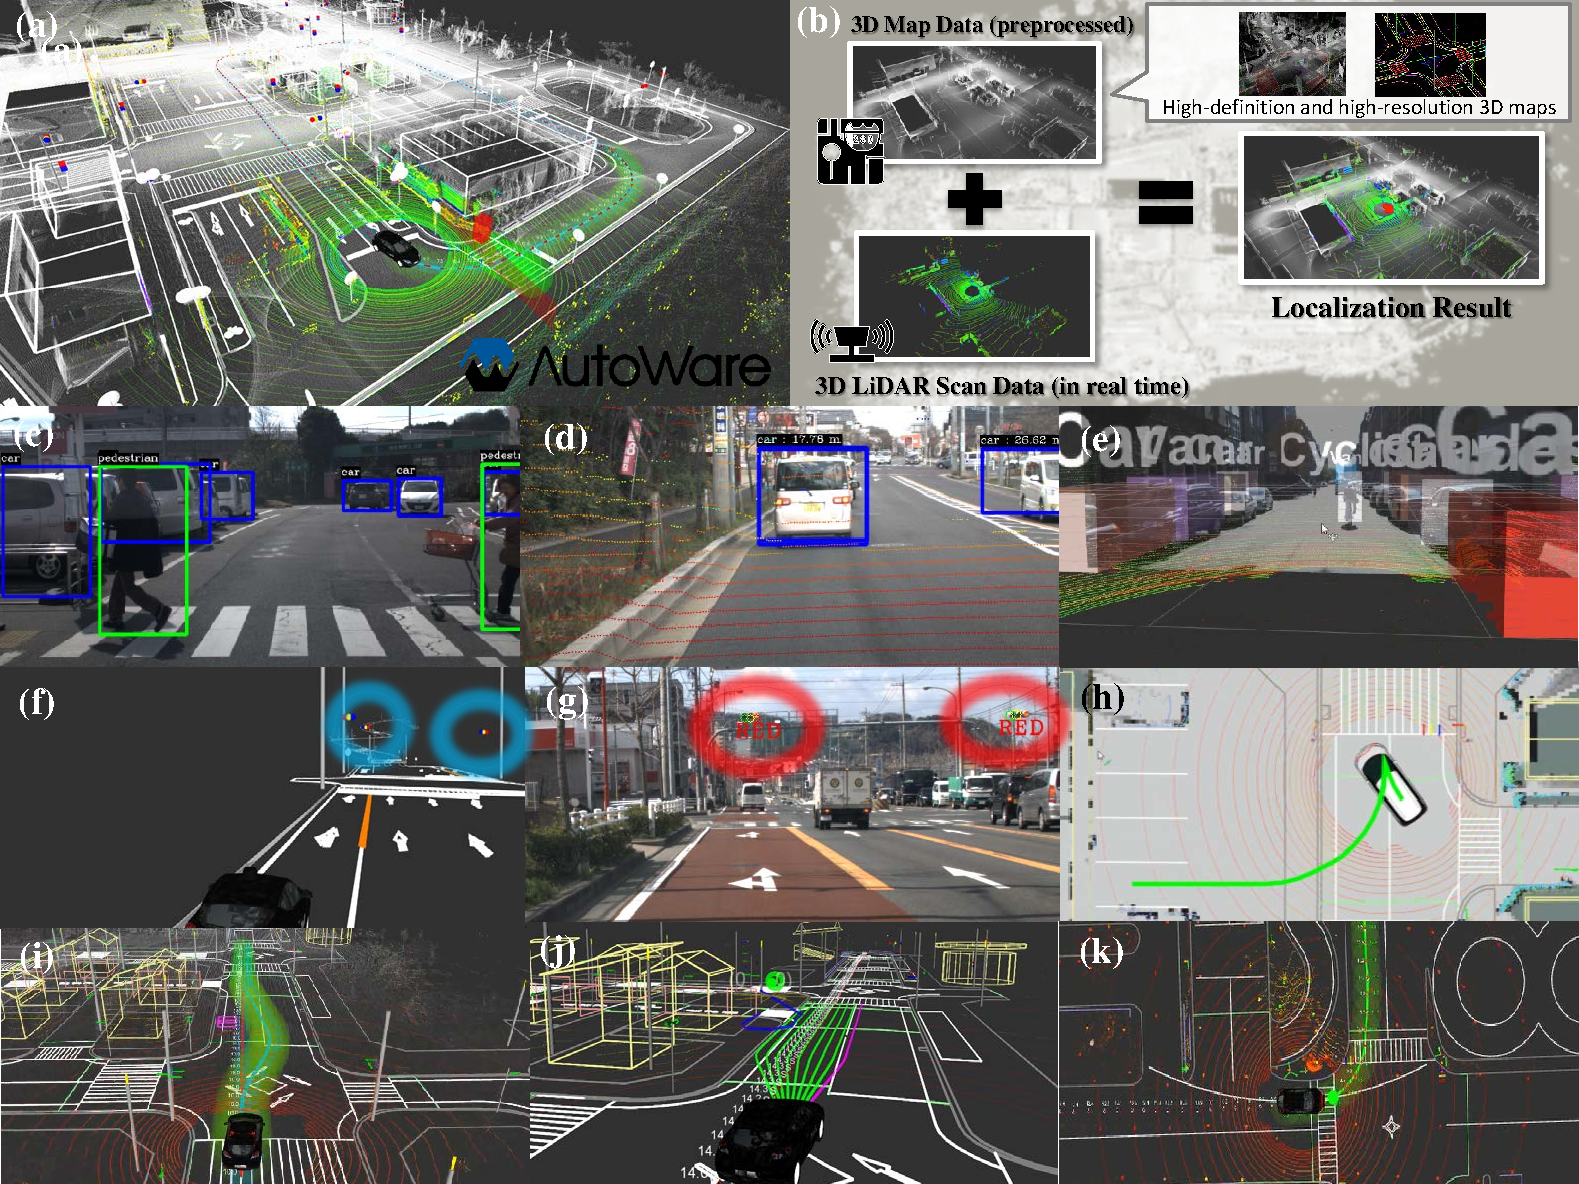
\includegraphics[width=1.0\linewidth]{../figure/rviz_autoware.eps}
  \caption{\label{fig:rviz_autoware}
  Self-driving software packages in Autoware:
  (a) RViz visualization with high-definition and high-resolution geographical information,
  (b) NDT scan matching localization using a 3D map and a 3D LiDAR scan,
  (c) deep learning based object detection with SSD, 
  (d) projection of the 3D point-cloud data onto the image, 
  (e) sensor fusion between the LiDAR sensor and the camera with calibration,
  (f) obtainment of the traffic light positions from the 3D map,
  (g) traffic light recognition with the ROI,
  (h) trajectory generation for parking lots using the hybrid-state A* search,
  (i) trajectory generation for object avoidance using the hybrid-state A* search,
  (j) trajectory generation for object avoidance using the lattice-based algorithm,
  (k) steering angular velocity calculation for path following using the pure pursuit algorithm.}
\end{figure*}



%%%%%%%%%%%% Acknowledgement %%%%%%%%%%%%%%%%%%%%%%%%%%%%%%%%%%%%%%%

\begin{acknowledgement}
  I would like to express my deep sense of gratitude to my adviser Professor Toshimitsu Ushio and Assistant Professor Takuya Azumi, Graduate School of Engineering Science, Osaka University, for their invaluable, constructive advice and constant encouragement during this work.
  Professor Ushio and Assistant Professor Azumi's deep knowledge and their eyes for detail have inspired me much.
  Without thier encouragement, this thesis would not have materialized.
  Assistant professor Azumi's deep knowledge and his eye for detail have inspired me much.

  I am deeply grateful to Associate Professor Shinpei Kato, Graduate School of Information Science and Technology, the University of Tokyo, Atsushi Matsuo, and Masaki Gondo, eSOL Inc, for their helpful comments on this thesis and warm encouragement.
  I also would like to thank all members of Ushio Laboratory for thier kind help and cooperation.
  I am particularly grateful for the assistance given by research assistant Seiya Maeda, my colleage Shunsuke Hori, and Takuro Yamamoto.
\end{acknowledgement}


%%%%%%%%%%%% References %%%%%%%%%%%%%%%%%%%%%%%%%%%%%%%%%%%%%%%

\bibliographystyle{IEEEtran}
\bibliography{./reference.bib}


%%%%%%%%%%%% Publication List %%%%%%%%%%%%%%%%%%%%%%%%%%%%%%%%%%%%%%%
\chapter*{Publication List}
\addcontentsline{toc}{chapter}{Publication List}

\renewcommand{\labelenumi}{[\arabic{enumi}]}

\section*{Journal}
\begin{enumerate}
\item Y.Maruyama, S.Kato, and T.Azumi,
  ``{Scalable Parallel Computing on NoC-based Embedded Many-Core Platform},''
  \emph{IEEE Transactions on Computers}, 2018.
  (submitted)
\end{enumerate}

\section*{International Conference Proceedings}
\begin{enumerate}
\item Y.Maruyama, S.Kato, and T.Azumi,
  ``{Exploring the Performance of ROS2},''
  \emph{In Proceedings of the 13th ACM International Conference on Embedded Software (EMSOFT2016)}, pp. 5, 2016.
\item Y.Maruyama, S.Kato, and T.Azumi,
  ``{Exploring Scalable Data Allocation and Parallel Computing on NoC-based Embedded Many Cores},''
  \emph{In Proceedings of the IEEE 35th International Conference on Computer Design (ICCD2017)}, pp. 225-228, 2017.
\item S.Kato, S.Tokunaga, Y.Maruyama, S.Maeda, M.Hirabayashi, Y.Kitsukawa, A.Monrroy, T.Ando, Y.Fujii, and T.Azumi,
  ``{Autoware on Board: Enabling Autonomous Vehicles with Embedded Systems},''
  \emph{In Proceedings of the the ACM/IEEE 9th International Conference on Cyber-Physical Systems (ICCPS2018)}, 2018.
\end{enumerate}

\section*{Domestic Conference}
\begin{enumerate}
\item Y.Maruyama, S.Kato, and T.Azumi,
  ``{Scalable Data Allocation and Parallel Computing on NoC-based Embedded Many Cores},''
  \emph{In Proceedings of IPSJ Kansai-Branch Convention}, A-2, 2017.
  (in Japanese)
\end{enumerate}

\end{document}

